\documentclass[12pt]{report}
\usepackage[margin=1in]{geometry}
\usepackage[compact,raggedright]{titlesec}
\usepackage{setspace} % for single/doublespacing commands
\usepackage{graphicx} % including graphics
% \usepackage{sectsty} % sexy section headings
\usepackage{pdfpages} % including multipage pdfs
\usepackage[export]{adjustbox} % for graphic frames and center
\usepackage{siunitx}
\usepackage[numbered]{matlab-prettifier} % including matlab w/ syntax highlighting
\usepackage[T1]{fontenc} % prettier matlab font
\usepackage{xfrac} % more legible inline fractions (\sfrac)
\usepackage{lmodern} % font package for above
\usepackage{multicol} % multiple columns
\usepackage[justification=centering]{caption} % figure captions (force centering)
\usepackage{amsmath} % more math symbols and shit
\usepackage{enumitem} % add arguments for enumerate to change style
\usepackage{subcaption} % subfigures with list of figure support
% \usepackage{subfigure}
\usepackage{multirow}
\usepackage{mathtools}
\usepackage{booktabs}
\usepackage{color}
\usepackage{ulem}
\usepackage{blindtext}
\usepackage[numbers]{natbib}
\usepackage{contour}
\usepackage{tabularx}
\usepackage{circuitikz} % drawing fancy shit
\usepackage{cancel} % arrow and cross math cancel symbol
\usepackage{lineno}
\usepackage{framed}
\usepackage{amssymb} % special math symbols
\usepackage{listings}
\usepackage{array}
\usepackage{BOONDOX-cal} % fancy mathtype script
\usepackage{fancyhdr}
\usepackage{flowchart}
\usepackage{color, colortbl}
\usepackage{tocloft}
\usepackage{url}
\usepackage{etoolbox}
\usepackage[usestackEOL]{stackengine}
\usepackage{caption}
% \usepackage{hyperref}

\setlength{\parskip}{\baselineskip}%
\setlength{\parindent}{0pt}%

\setcounter{secnumdepth}{5}
\renewcommand{\bibname}{References}
\sisetup{output-exponent-marker=\ensuremath{\mathrm{e}}}
\newcommand{\PreserveBackslash}[1]{\let\temp=\\#1\let\\=\temp}
\newcolumntype{C}[1]{>{\PreserveBackslash\centering}p{#1}}
\newcolumntype{R}[1]{>{\PreserveBackslash\raggedleft}p{#1}}
\newcolumntype{L}[1]{>{\PreserveBackslash\raggedright}p{#1}}
\lstMakeShortInline[style=Matlab-editor]| % matlab inline escape character
\graphicspath{{images/}}
\renewcommand\thesection{\arabic{section}}
\renewcommand\labelitemi{---}
\lstset{numberstyle=\ttfamily\small\color{gray}}
\renewcommand\linenumberfont{\ttfamily\small\color{gray}}
\setlength\linenumbersep{6mm}
\hbadness=99999  % or any number >=10000
\apptocmd{\sloppy}{\hbadness 10000\relax}{}{}
\usetikzlibrary{arrows,calc,patterns,angles,quotes}
% \usetikzlibrary{shapes.geometric}
% \usetikzlibrary{decorations.pathmorphing,decorations.pathreplacing} % for snakes!
% \usetikzlibrary{positioning, circuits.logic.US}
\newcommand{\Lag}{\mathcal{L}} % lagrangian L

\apptocmd{\sloppy}{\hbadness 10000\relax}{}{}
\setlength{\cftbeforetoctitleskip}{-2em}
\setlength{\cftbeforeloftitleskip}{-2em}
\setlength{\cftbeforelottitleskip}{-2em}
% \allsectionsfont{\raggedright} % w/ secsty
\setlist[enumerate]{wide=0pt, widest=99,
                    leftmargin=\parindent,topsep=0pt,partopsep=0pt,
                    label=\thesubsubsection.\alph*,font=\itshape}

\newcommand{\hiddensubsection}[1]{
  \stepcounter{subsection}
  \subsection*{\arabic{section}.\arabic{subsection}\hspace{1em}{#1}}
}
\newcommand{\hiddenappsec}[1]{
  \stepcounter{section}
  \subsection*{\Alph{section}\hspace{1em}{#1}}
}
\newcommand{\hiddenappsub}[1]{
  \stepcounter{subsection}
  \subsection*{\Alph{section}.\Roman{subsection}\hspace{1em}{#1}}
}

\titlespacing\section{0pt}{0pt}{-5pt}
\titlespacing\subsection{0pt}{0pt}{-5pt}
\titlespacing\subsubsection{0pt}{0pt}{-5pt}

\AtBeginEnvironment{thebibliography}{\def\UrlFont{\normalfont\itshape}}

\DeclareCaptionFormat{cont}{#1 (cont.)#2#3\par}

\DeclareCaptionLabelFormat{r-parens}{Figure \thefigure#2:} %Define our custom label

% \captionsetup{font=footnotesize} % The general caption settings
\captionsetup[sub]{              % The subcaption settings
    labelformat=r-parens}        % Use our custom label format

% \renewcommand{\thesubfigure}{\thefigure\alph{subfigure}}
% \looseness=-1 % for one-liners bleeding off into the next page

\begin{document}
\normalem
\begin{titlepage}
\flushleft
\doublespacing
\Large
\textsc{Test Document} \\
\normalsize
Trey Dufrene, Zack Johnson, David Orcutt, Alan Wallingford, Ryan Warner
\vfill
\center
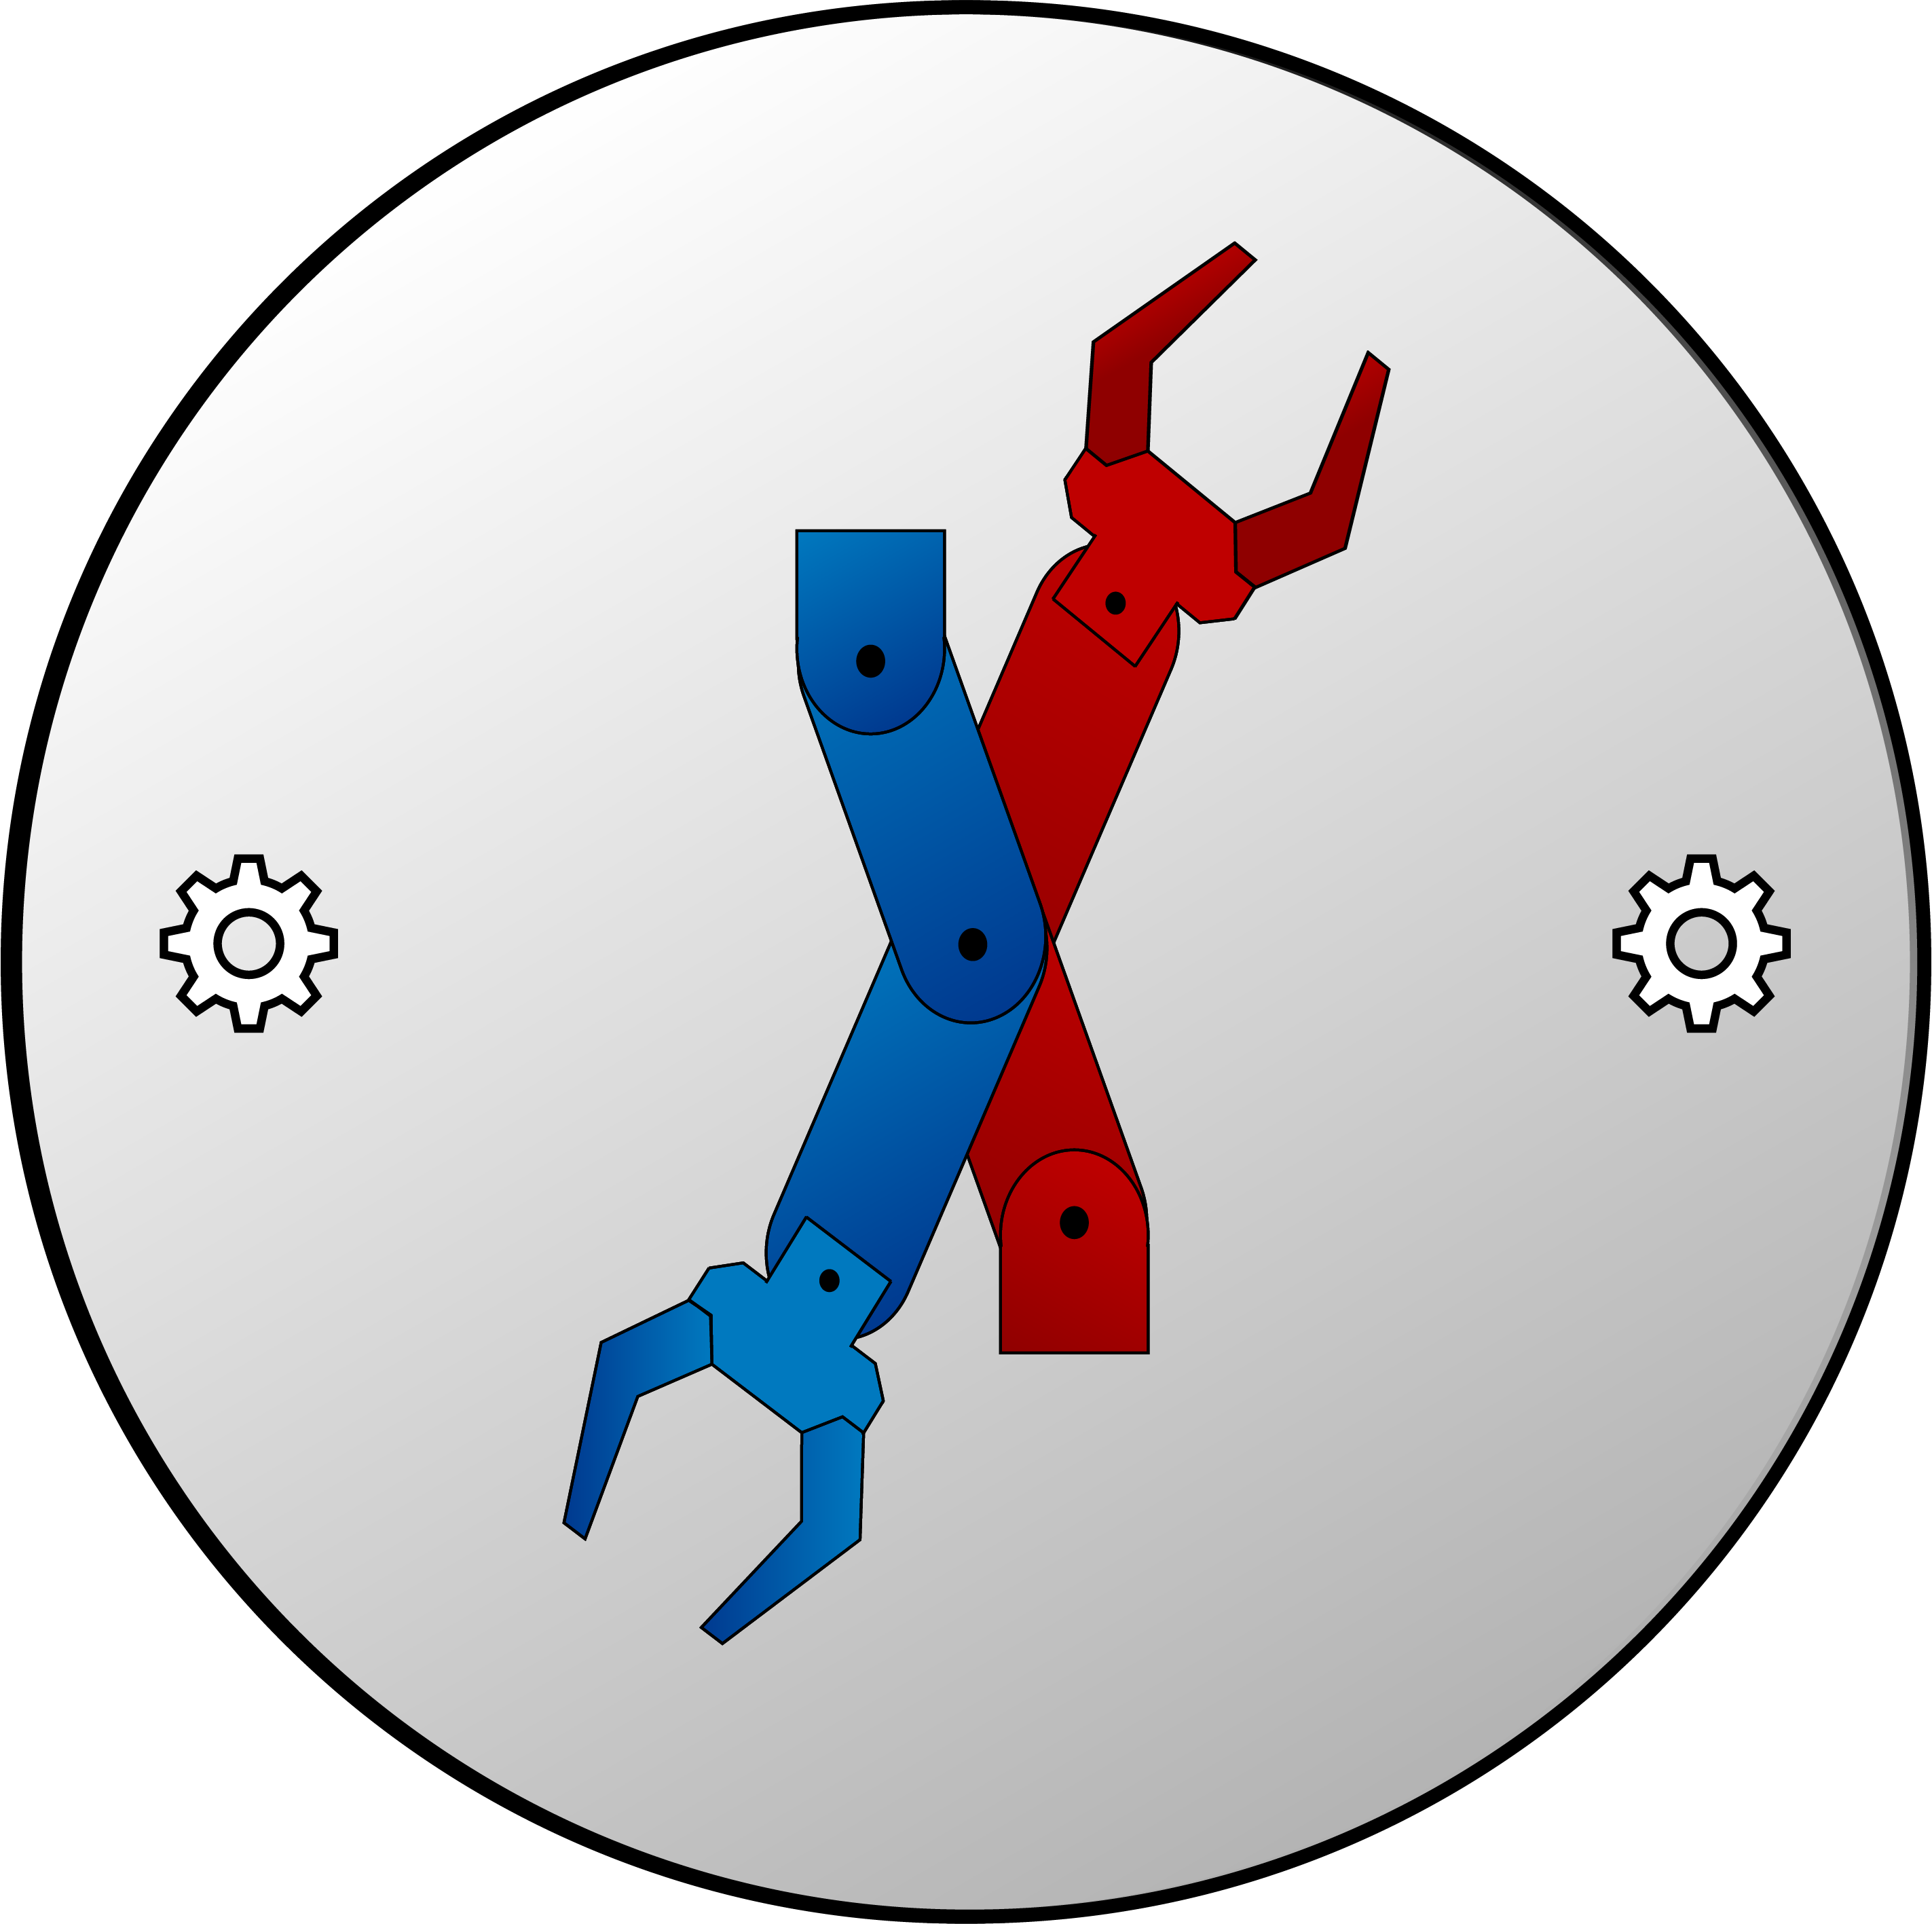
\includegraphics[width=.45\textwidth]{logo}
\vfill
\flushleft
ME 407 \\
Preliminary Design of Robotic Systems \\
Embry-Riddle Aeronautical University \\
\vspace{2ex}
\begin{minipage}[c]{.5\textwidth}
\flushleft

\includegraphics[width=.95\textwidth]{erau}
\end{minipage}%
\begin{minipage}[c]{.5\textwidth}
\flushright

\includegraphics[width=.8\textwidth]{text}
\end{minipage}
\end{titlepage}

\pagenumbering{roman}
\begin{abstract}
The Manipulator for Educational Institutions with Open Source Integrated Systems (MEIOSIS) aims to increase the accessibility of robotics to secondary educational institutions and hobbyists. Accordantly, the manipulator is 3D printed in PLA with aluminum tube supports and costs the end-user less than \$1000. The manipulator has six links and a base. The base houses a Raspberry Pi 3B and power supply. The Raspberry Pi controls seven Dynamixel smart servos with position feedback and proportional derivative control. Six MX-12W servos actuate six rotational joints, while one AX-12A servo actuates the removable end-effector. They provide the manipulator a position repeatability within 2mm of the previous pose. The manipulator can draw as well as perform pick and place operations within its dexterous workspace which is a hemispherical sub-shell of the reachable workspace of 280 mm thickness. The manipulator’s operation is controlled by open-source software.
\end{abstract}
% {\tableofcontents\let\clearpage\relax\listoffigures\let\clearpage\relax}
{\tableofcontents\clearpage\listoffigures\clearpage\listoftables}
\clearpage
\newpage
\section*{List Of Acronyms and Abbreviations}
\begin{tabular}{rcl}
  FK &:& Forward Kinematics \\
  IK &:& Inverse Kinematics  \\
  PD &:& Proportional Derivative \\
  % $k$~:& Spring constant \\
  % $h_{b}$~:& Distance to bar ($G$) from datum \\
  % $F_s$~:& Force onto bar due to spring\\
\end{tabular}

\section*{Notation}\vspace{-\baselineskip}
\renewcommand{\arraystretch}{2.25}
\begin{tabular}{rcl}
\large%
\(
{}^{\text{\scriptsize Frame}}_{\text{\scriptsize From}}~{r}~_{\text{\scriptsize To}}
\)\normalsize &:& Direction Vectors\\
\(
{}^{\text{\scriptsize From}}~{T}~_{\text{\scriptsize To}}
\)\normalsize &:& Direction Cosine (Transformation) Matrices \\
\(c_{\theta_{nm}}\)&:& \( \cos(\theta_n + \theta_m)\)\\
\(s_{\theta_{nm}}\)&:& \( \sin(\theta_n + \theta_m)\) \\
\end{tabular}
\renewcommand{\arraystretch}{1}
\newpage

\pagenumbering{arabic}
\section*{Preliminary and Detailed Design}
\section{Electrical System}
\section{Mechanical System}
\subsection*{Description of Mechanical Design}
One of the main differences between the conceptual mechanical design and the final design is the inclusion of 3D-printed harmonic gearboxes. The previous designs utilized a combination of standard spur gears and timing belts. It was determined that neither of these options provided the necessary precision without also introducing backlash into the system, which is nearly impossible to correct for with our feedback configuration. The solution was to design and implement a harmonic drive system. The harmonic gearbox locations are shown below in Figure \ref{fig:HarmonicGearboxLocations}

\begin{figure}[htp]
  \centering
  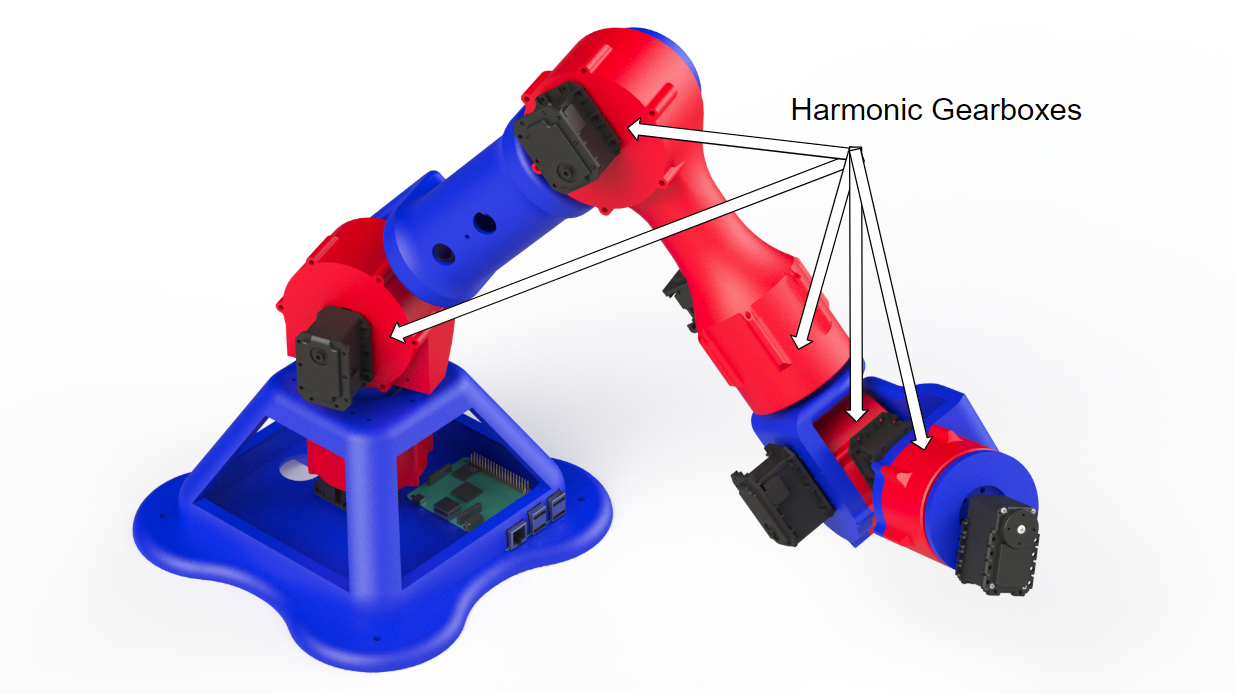
\includegraphics[width=.65\textwidth,frame]{HarmonicGearboxLocations}
  \caption{Harmonic Gearbox Locations}
  \label{fig:HarmonicGearboxLocations}
\end{figure}

As seen in Figure \ref{fig:HarmonicGearboxLocations}, each joint only requires a single actuator, which is a configuration not seen in the previous design. This is possible because harmonic drives allow for very high gear ratios with minimal backlash. The first prototype harmonic drive was provided by a posting on Thingiverse [citation]. This design was meant to be driven by a stepper motor and provided a gear ratio of 39:1. However, the gearboxes implemented in the manipulator need to be driven by a smart servo. Because the smart servo cannot drive as fast as a stepper motor, the ratio of 39:1 resulted in joint movement that was extremely slow. Additionally, given the link lengths and precision of the servos, only a gear ratio of 20:1 was necessary to meet the precision requirements of the system. For these reasons, a second harmonic drive was designed to provide the proper gear ratio of 20:1. Figure \ref{fig:ExplodedViewoftheHarmonicGearbox} provides an exploded view of the main structural components of the newest harmonic drive.

\begin{figure}[htp]
  \centering
  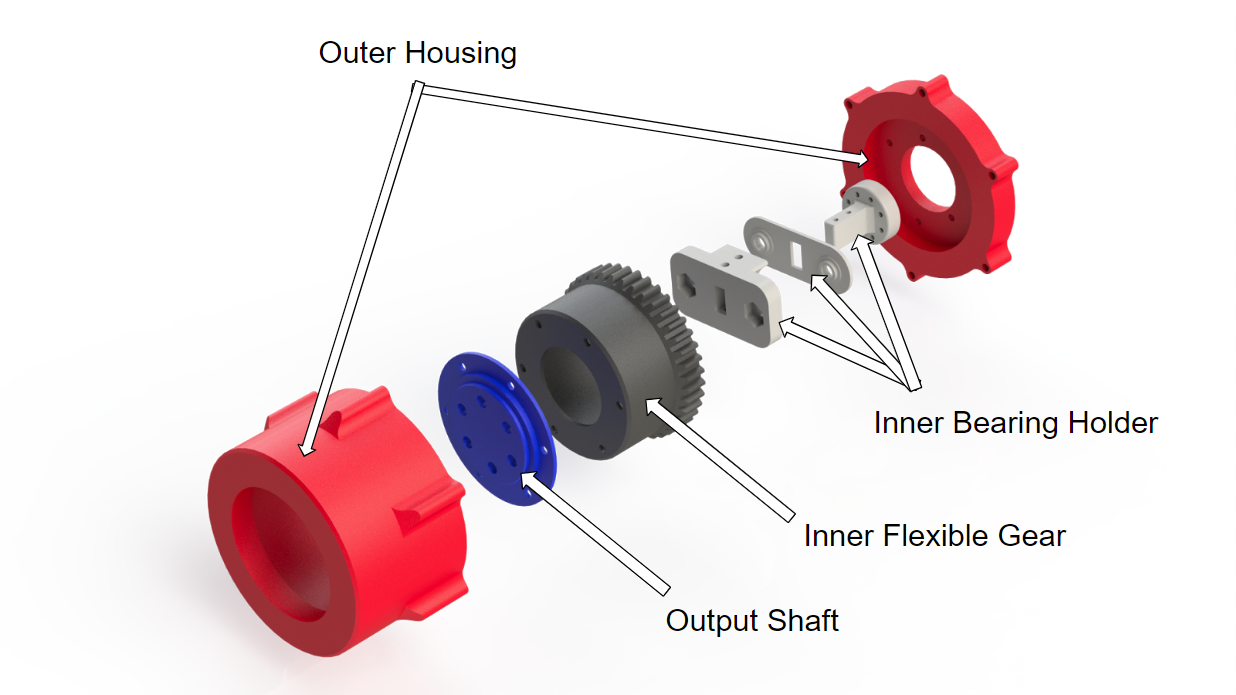
\includegraphics[width=.65\textwidth,frame]{ExplodedViewoftheHarmonicGearbox}
  \caption{ExplodedViewoftheHarmonicGearbox}
  \label{fig:ExplodedViewoftheHarmonicGearbox}
\end{figure}

As seen in Figure \ref{fig:ExplodedViewoftheHarmonicGearbox}, the basic harmonic drive design features an outer housing, a stiff output shaft, a flexible gear, and a bearing holder assembly. When fully assembled, the bearing holder sits on the inside of the flexible gear. As the servo drives the inner bearing holder, a continuous meshing of teeth occurs between the flexible gear and the set of teeth that are built into the outer housing. Because the inner set of teeth has two less teeth than the outer set (the inside has 40 while the outside has 42), the inner gear will move forward by two teeth per rotation of the bearing holder. This results in 1/20th of a rotation of the flexible gear per full rotation of the bearing holder. With the output shaft being attached to the flexible gear, the whole harmonic drive provides a ratio of 20:1.

\subsubsection*{Equations of Motion}
Given robot dynamics described by \(H(\gamma) \ddot{\gamma}+d(\gamma, \dot{\gamma})+G(\gamma)=F_{\gamma},\) the equations of motion for
the manipulator can be determined. Solving this equation for the acceleration, \(\ddot{\gamma}\), gives:
\begin{equation}
  \ddot{\gamma}=H(\gamma)^{-1}\left(F_{\gamma}-d(\gamma, \dot{\gamma})-G(\gamma)\right)
  \label{eq:eoms}
\end{equation}
Where $H$ is the system mass matrix, $F_{\gamma}$ is the vector of generalized forces, $d$ is the vector of centripital and coriolis effects, and $G$ is gravitational effects.
\[
  \renewcommand{\arraystretch}{1.5}
  H(\gamma) = \sum_B^N J_B(\gamma)^T
  \begin{bmatrix}
    ^B_BJ & \mathring{S}(^B_B\Gamma) ^IT_B^T\\
    ^IT_B\mathring{S}(^B_B\Gamma)^T & m_BI
  \end{bmatrix}
  J_B(\gamma)~,\quad
  ^B_B\Gamma = ^B_Br_{cm}m_b~,\quad \mathring{S}(\omega)r=(\omega\times r)
\]
\[
  \renewcommand{\arraystretch}{1.5}
  d(\gamma,\dot{\gamma}) = \sum_B^N J_B(\gamma)^T
  \begin{bmatrix}
    ^B_BJ & \mathring{S}(^B_B\Gamma) ^IT_B^T\\
    ^IT_B\mathring{S}(^B_B\Gamma)^T & m_BI
  \end{bmatrix}
  \dot{J}_B(\gamma,\dot{\gamma})\dot{\gamma}+J_B(\gamma)^T
  \begin{bmatrix}
    ^B_B\omega_I \times ^B_BJ ^B_B\omega_I \\
    ^IT_B\left(^B_B\omega_I\times(^B_B\omega_I\times^B_B\Gamma)\right)
  \end{bmatrix}
\]
\[
G(\gamma) = \left(\frac{\partial U(^Ir(\gamma))}{\partial\gamma}\right)^T~,\quad U_B = \begin{bmatrix} 0 & 0 & g\end{bmatrix}\left(^I_Br_Bm_B + ^IT_B{}_B^B\Gamma\right)
\]
Where $J_B$ is the jacobian of the body, $\Gamma$ is the vector of first mass moments, $m_B$ is the mass of the body, and $^B_B\omega_I$ is the rotational velocity of the body relative to the inertial frame.
\subsubsection*{Actuator Dynamics}
Given robot dynamics described by \(H(\gamma)\ddot{\gamma} + n(\gamma,\dot{\gamma}) = \tau\), the torque, $\tau$, provided by the servo motors is necessary to solve the closed loop dynamics of the system. Assuming the servo is driven by a D.C. motor with proportional derivative control,
\begin{equation}
  \tau_a = Ki_a = J_a\ddot{\theta}_a + b_a\dot{\theta}_a + \tau_L
  \label{eq:motor}
\end{equation}
Where $\tau_a$ is the actuator torque, $K$ is the back-EMF constant, $i_a$ is the motor current, $J_a$ is the armature inertia, $\theta_a,~\dot{\theta}_a,\ddot{\theta}_a$ is the motor position and it's first and second time derivatives respectively, $b_a$ is the viscous friction coefficient, and $\tau_L$ is the torque available for the actuator to do work. The basic equation for a motor is known to be:
\begin{equation}
  V_a = i_aR_a + K\dot{\theta}_a
  \label{eq:va}
\end{equation}
Where $V_a$ is the voltage applied to the actuator and $R_a$ is the armature resistance. Given a gearbox with $\sfrac{\text{in}}{\text{out}}$ ratio $N$ and efficiency $\eta$,
\begin{center}
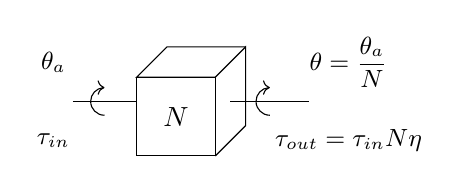
\begin{tikzpicture}
\pgfmathsetmacro{\cubex}{1}
\pgfmathsetmacro{\cubey}{1}
\pgfmathsetmacro{\cubez}{1}
\draw (0,0,0) -- ++(-\cubex,0,0) -- ++(0,-\cubey,0) -- ++(\cubex,0,0) -- cycle;
\draw (0,0,0) -- ++(0,0,-\cubez) -- ++(0,-\cubey,0) -- ++(0,0,\cubez);
\draw (0,0,0) -- ++(-\cubex,0,0) -- ++(0,0,-\cubez) -- ++(\cubex,0,0);
\draw (-2,-.5,-.5) -- ++(.8,0,0) node(a)[midway,above]{} node(b)[midway]{} node(c)[midway,below]{};
\pic [draw,angle radius=5,<-] {angle = a--b--c};
\node at (-2.25,0,-.5) {\small $\theta_a$};
\node at (-2.25,-1,-.5) {\small $\tau_{in}$};
\draw (0,-.5,-.5) -- ++(1,0,0);
\draw (0,-.5,-.5) -- ++(1,0,0) node(a1)[midway,above]{} node(b1)[midway]{} node(c1)[midway,below]{};
\pic [draw,angle radius=5,<-] {angle = a1--b1--c1};
\node at (1.5,0,-.5) {\small $\theta=\dfrac{\theta_a}{N}$};
\node at (1.5,-1,-.5) {\small $\tau_{out}=\tau_{in}N\eta$};
\node at (-.5,-.5,0) {$N$};
\end{tikzpicture}
\end{center}

The motor equation (\ref{eq:motor}) can be expressed in the output coordinates:
\[
Ki_a = J_aN\ddot{\theta} + b_aN\dot{\theta} + \frac{\tau}{N\eta}
\]
Substituing into equation (\ref{eq:va}) and solving for $i_a$:
\[
  i_a = \frac{J_aN}{K}\ddot{\theta} + b_aN\dot{\theta} + \frac{\tau}{N\eta}
\]
\begin{equation}
  V_a = \frac{R_aJ_aN}{K}\ddot{\theta} + \frac{R_ab_aN}{K}\dot{\theta} + \frac{R_a}{KN\eta}\tau + KN\dot{\theta}
  \label{eq:newva}
\end{equation}
Assuming PD control, \(V_a = K_p(\theta-\theta_d) + K_d\dot{\theta}\), where $\theta_d$ is the desired orientation of the actuator, the following solution is found by setting the PD solution equal to (\ref{eq:newva}). After collecting like terms:

\begin{equation}
  \frac{R_aJ_aN}{K}\ddot{\theta} + \left( \frac{R_aJ_aN}{K} - K_d + KN \right)\dot{\theta} - K_p\theta = -K_p\theta_d - \frac{R_a}{KN\eta}\tau
  \label{eq:end1}
\end{equation}
\newpage
The following parameters of the system can be obtained by applying a step input to the system with $\tau=0$ and measuring the characteristics of it's response. Denoting $\zeta$ as the damping ratio and $\omega_n$ as the natural frequency of the system,
\[
  \text{\% Overshoot} = \left( \frac{\theta_{max} - \theta_{ss}}{\theta_{ss}} \right) \times 100~,\quad \zeta = \frac{-\ln(\sfrac{\%\text{OS}}{100})}{\sqrt{\pi^2 + \ln^2(\sfrac{\%\text{OS}}{100})}}~,\quad \omega_n = \frac{\pi}{T_p\sqrt{1-\zeta^2}}
\]

Given $\theta_{max},~\theta_{ss},$ and $T_p$ as measured parameters of the system's max output, steady state, and time to peak, respectively.

Refactoring equation (\ref{eq:end1}) and equating with the general solution for a second order system given by $\ddot{\theta} + 2\zeta\omega_n\dot{\theta} + \omega_n^2\theta = \omega_n^2\theta_d$, the following solutions are found:

\begin{minipage}[c]{.5\textwidth}
\begin{equation}
  2\zeta\omega_n = \frac{b_a}{J_a} - \frac{KK_d}{R_aJ_aN} + \frac{K^2}{R_aJ_a}
  \label{eq:one}
\end{equation}
\end{minipage}%
\begin{minipage}[c]{.5\textwidth}
\begin{equation}
  \omega_n^2 = \frac{-KK_p}{R_aJ_aN}
  \label{eq:two}
\end{equation}
\end{minipage}

Performing a similar experiment as previously described, except with a known inertial load $\tau = J_m\ddot{\theta}$, the following parameters can be found:
\[
  \alpha_m \equiv 2\zeta\omega_n = \frac{R_ab_aN^2\eta-KK_dN\eta+K^2N^2\eta}{R_aJ_aN^2\eta+R_aJ_m}~,\quad
  \beta_m \equiv \omega_n =-\frac{KK_pN\eta}{R_aJ_aN^2\eta+R_aJ_m}
\]

\begin{equation}
\begin{bmatrix}
  1 & -(\alpha_1J_1+\beta_1J_1) \\
  1 & -(\alpha_2J_2+\beta_2J_2) \\
  \vdots & \vdots
\end{bmatrix}
\begin{bmatrix}
  \dfrac{R_ab_aN^2\eta-KK_dN\eta+K^2N^2\eta-KK_pN\eta}{R_aJ_aN^2\eta} \\
  ~\\
  \dfrac{1}{J_aN^2\eta}
\end{bmatrix}
=
\begin{bmatrix}
  \alpha_1+\beta_1 \\
  \alpha_2+\beta_2 \\
  \vdots
\end{bmatrix}
\label{eq:soe}
\end{equation}
With multiple datasets (varying inertial loads, $J_m$), the solutions of (\ref{eq:soe}) can be found using the least-squares method, yeilding

\begin{minipage}[c]{.5\textwidth}
\begin{equation}
  \frac{R_ab_aN-KK_d+K^2N\eta-KK_p}{R_aJ_aN}
  \label{eq:three}
\end{equation}
\end{minipage}%
\begin{minipage}[c]{.5\textwidth}
\begin{equation}
  \frac{1}{J_aN^2\eta}
  \label{eq:four}
\end{equation}
\end{minipage}

Finally, the coefficients of the second order system (\ref{eq:fin}) are known:
\begin{equation}
  \underbrace{\bigg(J_aN^2\eta\bigg)}_{\scalebox{1.25}{\sfrac{1}{(\ref{eq:four})}}}\ddot{\theta} + \underbrace{\left(\frac{R_ab_aN^2\eta - KK_dN\eta + K^2N^2\eta}{R_a}\right)}_{\quad\scalebox{1.25}{\sfrac{(\ref{eq:one})}{(\ref{eq:four})}}}
  \dot{\theta} - \underbrace{\left(\frac{KK_pN\eta}{R_a}\right)}_{\scalebox{1.25}{\sfrac{(\ref{eq:two})}{(\ref{eq:four})}}}
  \theta + \underbrace{\left(\frac{KK_pN\eta}{R_a}\right)}_{\scalebox{1.25}{\sfrac{(\ref{eq:two})}{(\ref{eq:four})}}}
  \theta_d = -\tau
  \label{eq:fin}
\end{equation}
The MATLAB code implementing this process can be found in the Appendix (see section \ref{sec:app}, p. \pageref{sec:app}, \emph{Listing \ref{code:mmodel}}).
\newpage
The torque provided by the servo can now be solved for, given the current position ($\theta$), velocity ($\dot{\theta}$), angular acceleration ($\ddot{\theta}$), and desired position ($\theta_d$) are known.

Given the complete equation for the dynamical response of the system (\ref{eq:dynamics}), substituting in the solution obtained for the motor dynamics and solving for the acceleration,
\begin{equation}
\left(H + J_aN^2\eta\right)^{-1} \left[\left(B - \frac{R_ab_aN^2\eta - KK_dN\eta + K^2N^2\eta}{R_a}\right)\dot{\gamma} - \left(\frac{KK_pN\eta}{R_a}\right)(\gamma_d - \gamma) - n\right]= \ddot{\gamma}
\end{equation}
Where
\[
n(\gamma,\dot{\gamma}) = d(\gamma,\dot{\gamma}) + G(\gamma) + C\text{sgn}(\dot{\gamma})
\]
\newpage


% \subsection{Closed-Loop Simulation}
The motor equation (\ref{eq:fin}) gives an expression for the motor torques, however the system dynamics are defined in terms of geometric joint angles. The inclusion of differential drive systems means that the joint angles, $\gamma$, do not directly correspond to motor rotations, $\theta$, as shown in \emph{Figure \ref{fig:motorloc}}.


\begin{figure}[htp]
  \center
  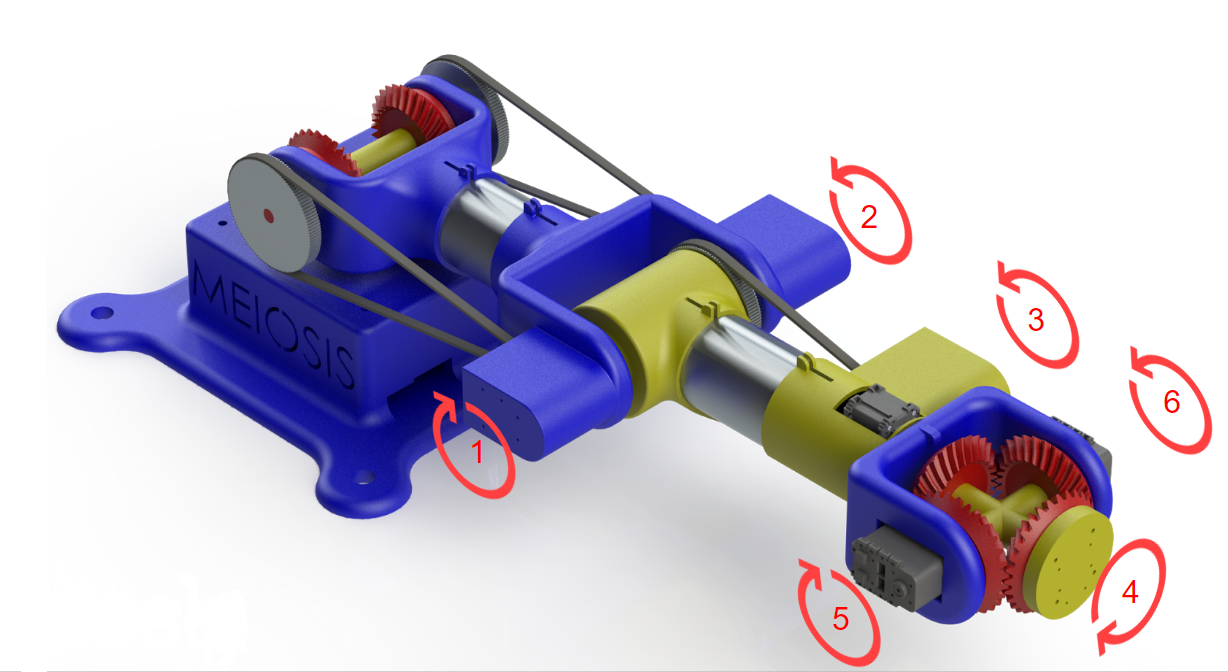
\includegraphics[width=.75\textwidth,frame]{motorloc}
  \caption{Motor Locations and Orientations}
  \label{fig:motorloc}
\end{figure}

\emph{Figure \ref{fig:motorloc}} shows the motor positions and relative orientations.
This layout was used to define a linear relation between the joint angles and the motor rotations, described in equation (\ref{eq:A}).

\begin{equation}
  \gamma = A\theta\quad \text{where}~~A=\left[\begin{array}{cccccc}{1 /(2 N)} & {1 /(2 N)} & {0} & {0} & {0} & {0} \\ {1 /(2 N)} & {-1 /(2 N)} & {0} & {0} & {0} & {0} \\ {0} & {0} & {-1 / N} & {0} & {0} & {0} \\ {0} & {0} & {0} & {1} & {0} & {0} \\ {0} & {0} & {0} & {0} & {-1 / 2} & {1 / 2} \\ {0} & {0} & {0} & {0} & {1 / 2} & {1 / 2}\end{array}\right]
\label{eq:A}
\end{equation}
Equation (\ref{eq:A}) can be used to map the joint angles to the motor angles. The gear ratio of 1:10 is represented by the variable N. Similarly, the motor angles can be determined by multiplying both sides of equation (\ref{eq:A}) by the inverse of matrix A, giving the following relation.
\begin{equation}
\theta=A^{-1} \gamma
\label{eq:Ainv}
\end{equation}
It is important to note that the virtual work done by the joint torques ($F_{\gamma}$) and the virtual work done by the motor torques ($F_{\theta}$) are equal. Using equation (\ref{eq:Ainv}), a linear relation between the joint torques and motor torques can be determined.
\[
\begin{aligned}
  \delta W = F_{\theta}^{T} \delta \theta&=F_{\gamma}^{T} \delta \gamma, \text { where } \delta \gamma=A \delta \theta \\
  F_{\theta}^{T} \delta \theta &= F_{\gamma}^{T}(A \delta \theta) \\
  F_{\theta}^{T}&=F_{\gamma}^{T} A\\
  \left(F_{\theta}^{T}\right)^{T}&=\left(F_{\gamma}^{T} A\right)^{T}\\
  F_{\theta}=A^{T} F_{\gamma} &\Leftrightarrow F_{\gamma}=A^{-T} F_{\theta}\qquad\quad
\end{aligned}
\]
Using this equation, a relation can be determined between the motor dynamics and the system dynamics given in equation (\ref{eq:fin}) and equation (\ref{eq:eoms}) respectively.

\[
H(\gamma) \ddot{\gamma}+d(\gamma, \dot{\gamma})+G(\gamma)=-A^{-T}\left(C_1A^{-1} \ddot{\gamma}+C_2 A^{-1} \dot{\gamma}+C_3 \theta_{d}- C_3A^{-1} \gamma\right)
\]
\begin{equation}
\ddot{\gamma}=H(\gamma)^{-1}\left(-A^{-T}\left(C_1 A^{-1} \ddot{\gamma}+C_2 A^{-1} \dot{\gamma}+C_3 \theta_{d}-C_3A^{-1} \gamma\right)-d(\gamma, \dot{\gamma})-G(\gamma)\right)
\label{eq:gddot}
\end{equation}

Because this equation includes the motor model, which in turn includes an internal PD controller, this equation can be integrated to solve for the system response given a desired motor angle input, $\theta_d$. However, doing so will not result in the desired system response. This control scheme does not have any compensation for the inertia of the links, and it is also lacking gravity compensation. This can be remedied by modifying the input to the motors, $\theta_d$. A new input, $u$, is defined such that gravity can be compensated. Thus, the motor input term in equation (\ref{eq:gddot}) must include both compensation for gravity and the desired motor angle.
\[
A^{-T} C_3  u=G(\gamma)+d(\gamma, \dot{\gamma})+A^{-T} C_3\theta_{d}
\]
\begin{equation}
u=\left(A^{-T} C_3\right)^{-1} \left(G(\gamma)+d(\gamma, \dot{\gamma})\right) + \theta_{d}
\end{equation}
With this new motor input, the closed loop control system equations of motion are given as:
\begin{equation}
\ddot{\gamma}=H(\gamma)^{-1}\left(-A^{-T}\left(C_1 A^{-1} \ddot{\gamma}+C_2 A^{-1} \dot{\gamma}+C_3 u-C_3A^{-1} \gamma\right)-d(\gamma, \dot{\gamma})-G(\gamma)\right)
\label{eq:gddotfin}
\end{equation}
Equation (\ref{eq:gddotfin}) can then be integrated to solve for the system response given desired motor angles.

\begin{figure}[htp]
  \center
  \begin{subfigure}[c]{0.33\textwidth}
    \center
    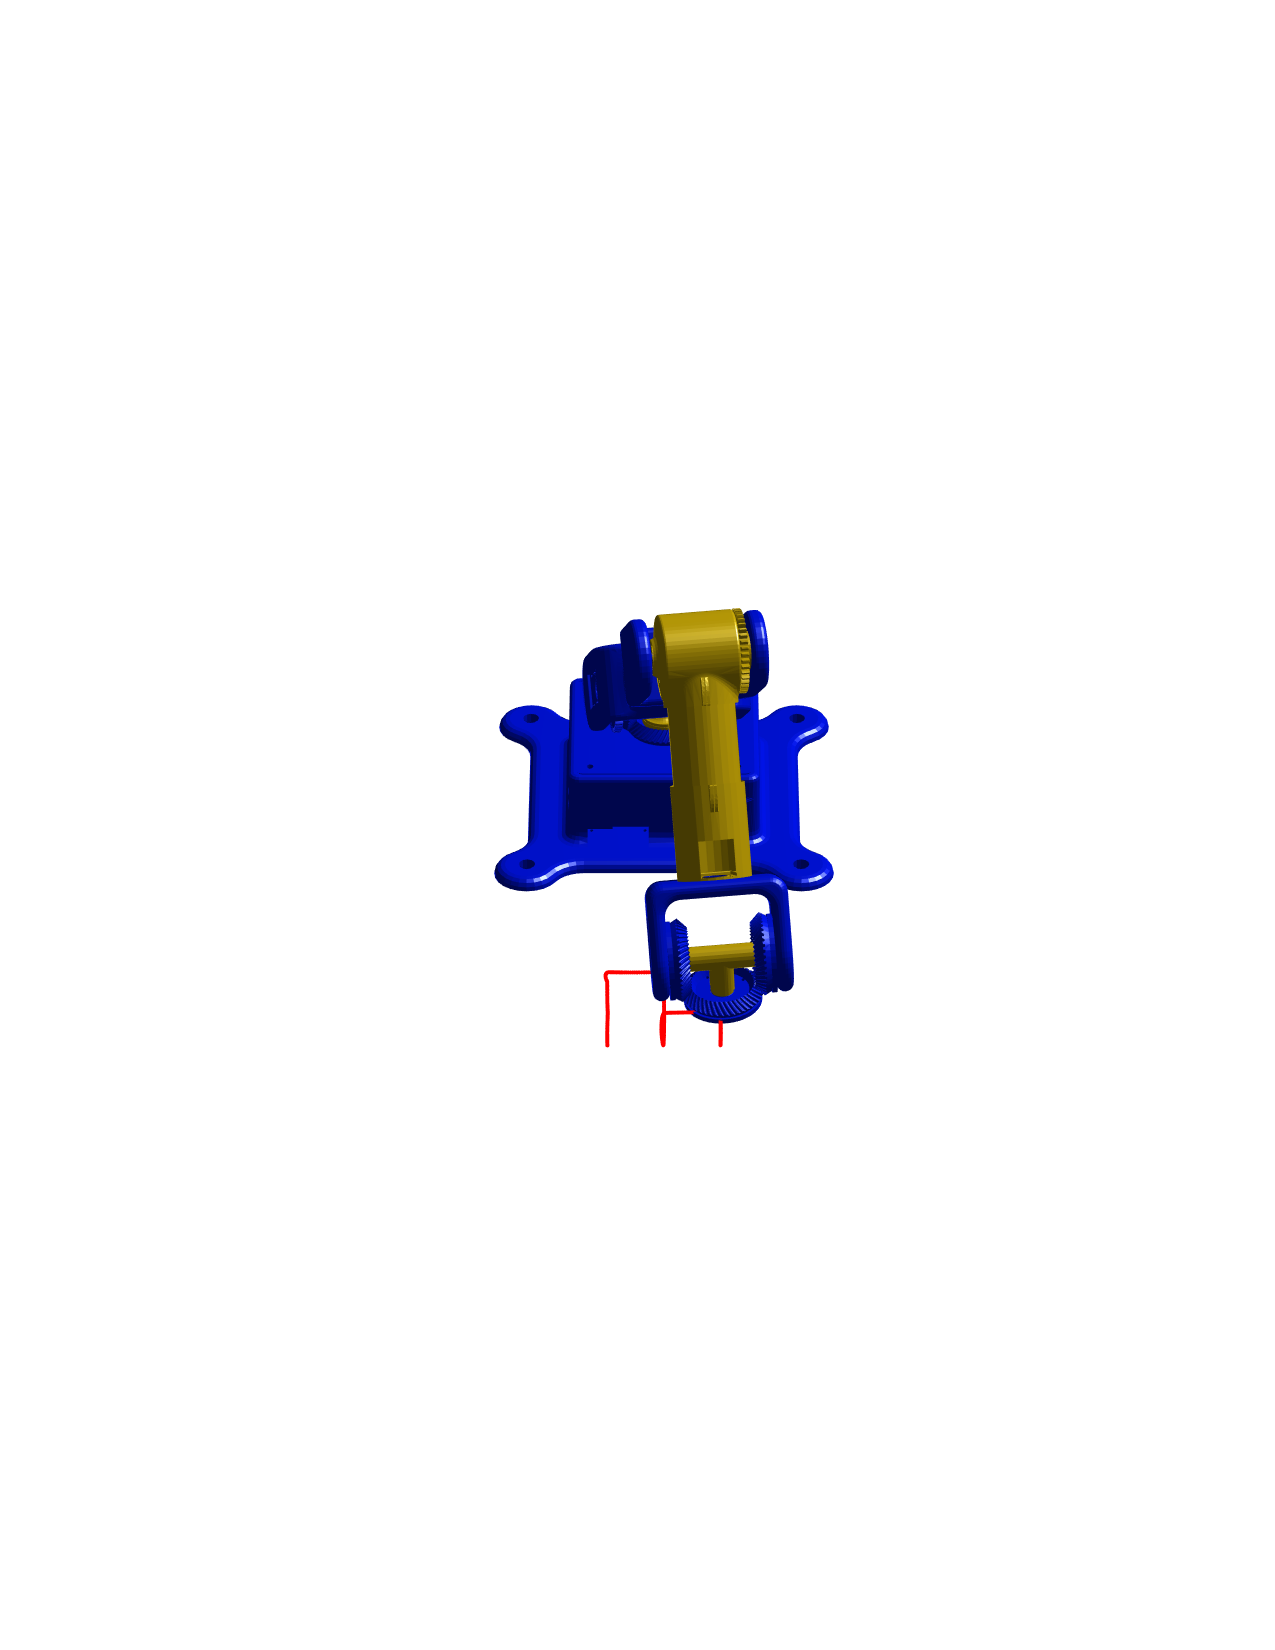
\includegraphics[width=.9\textwidth,frame]{clsnap1}
    \caption{Frame Snapshot near Simulation \\Initiation}
  \end{subfigure}%
  \begin{subfigure}[c]{0.33\textwidth}
    \center
    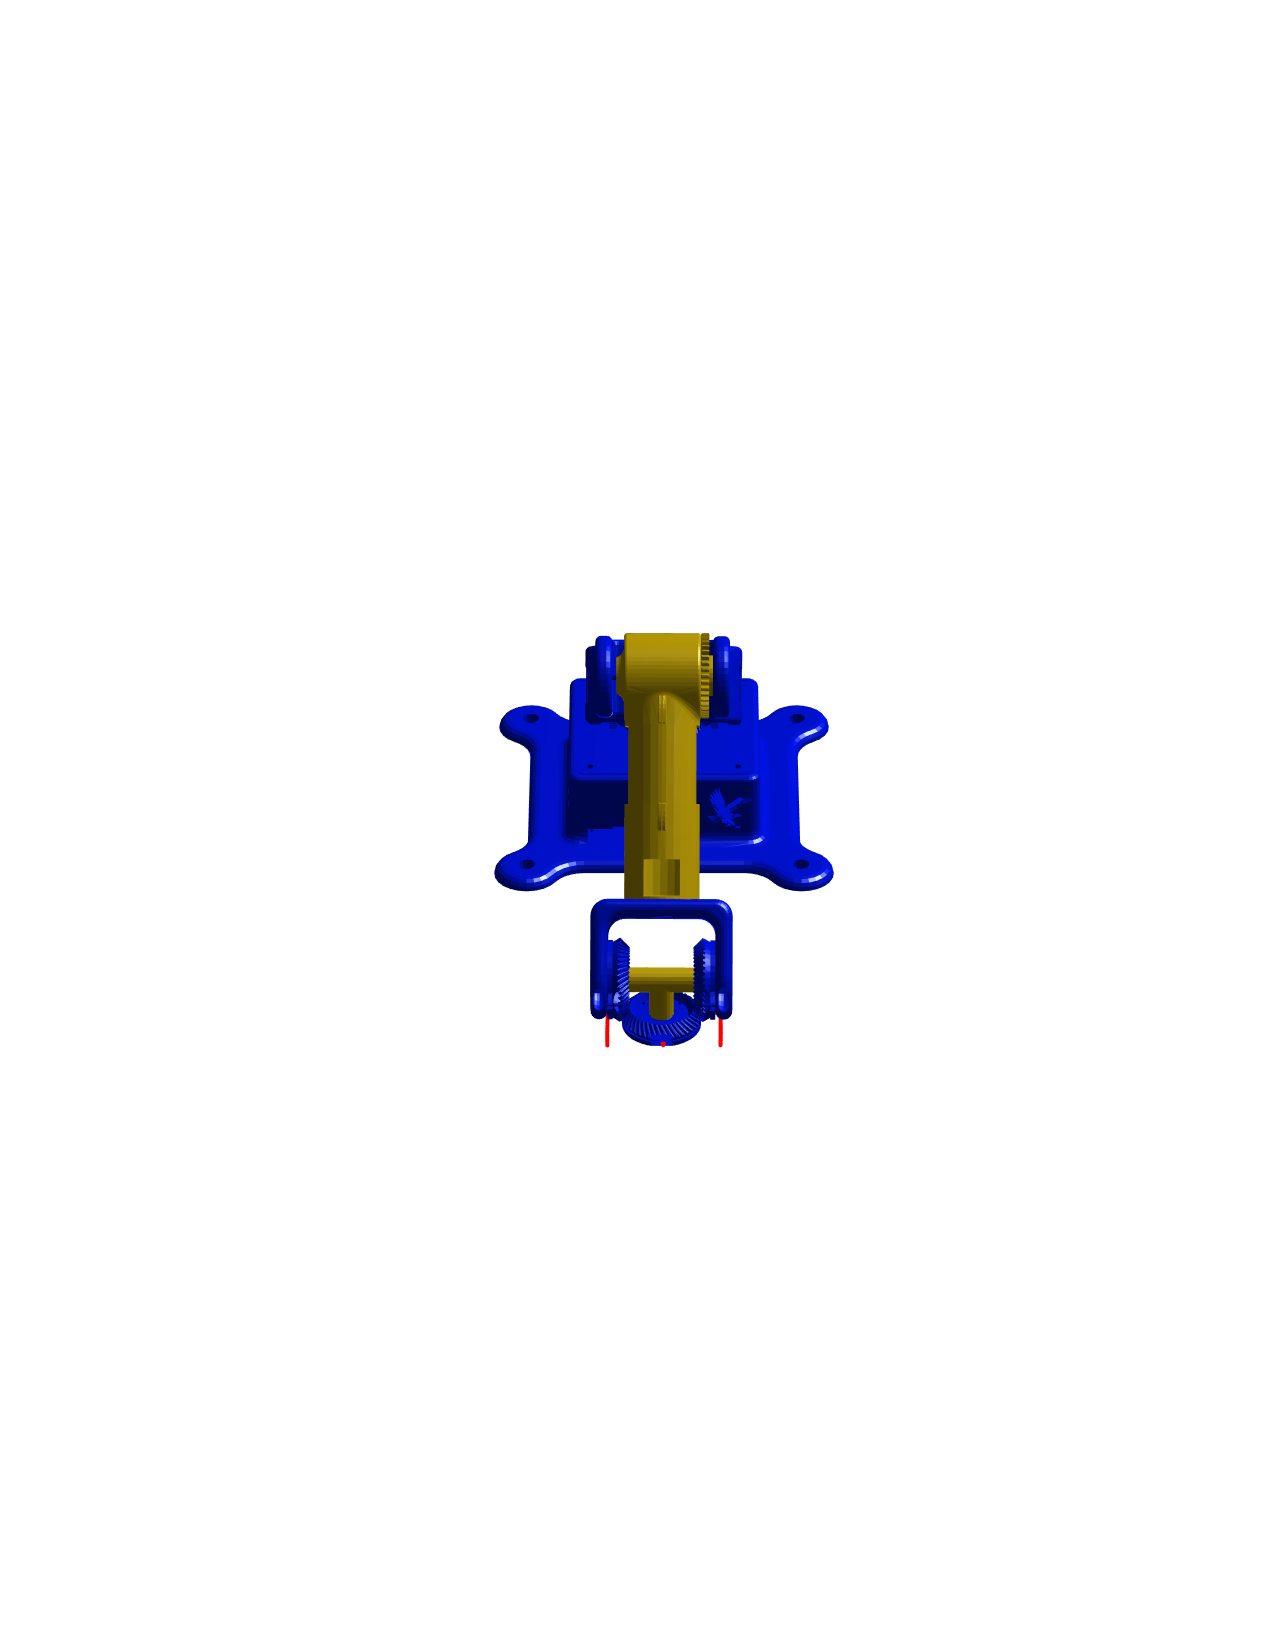
\includegraphics[width=.9\textwidth,frame]{clsnap2}
    \caption{Frame Snapshot near Simulation \\Middle}
  \end{subfigure}%
\begin{subfigure}[c]{0.33\textwidth}
  \center
  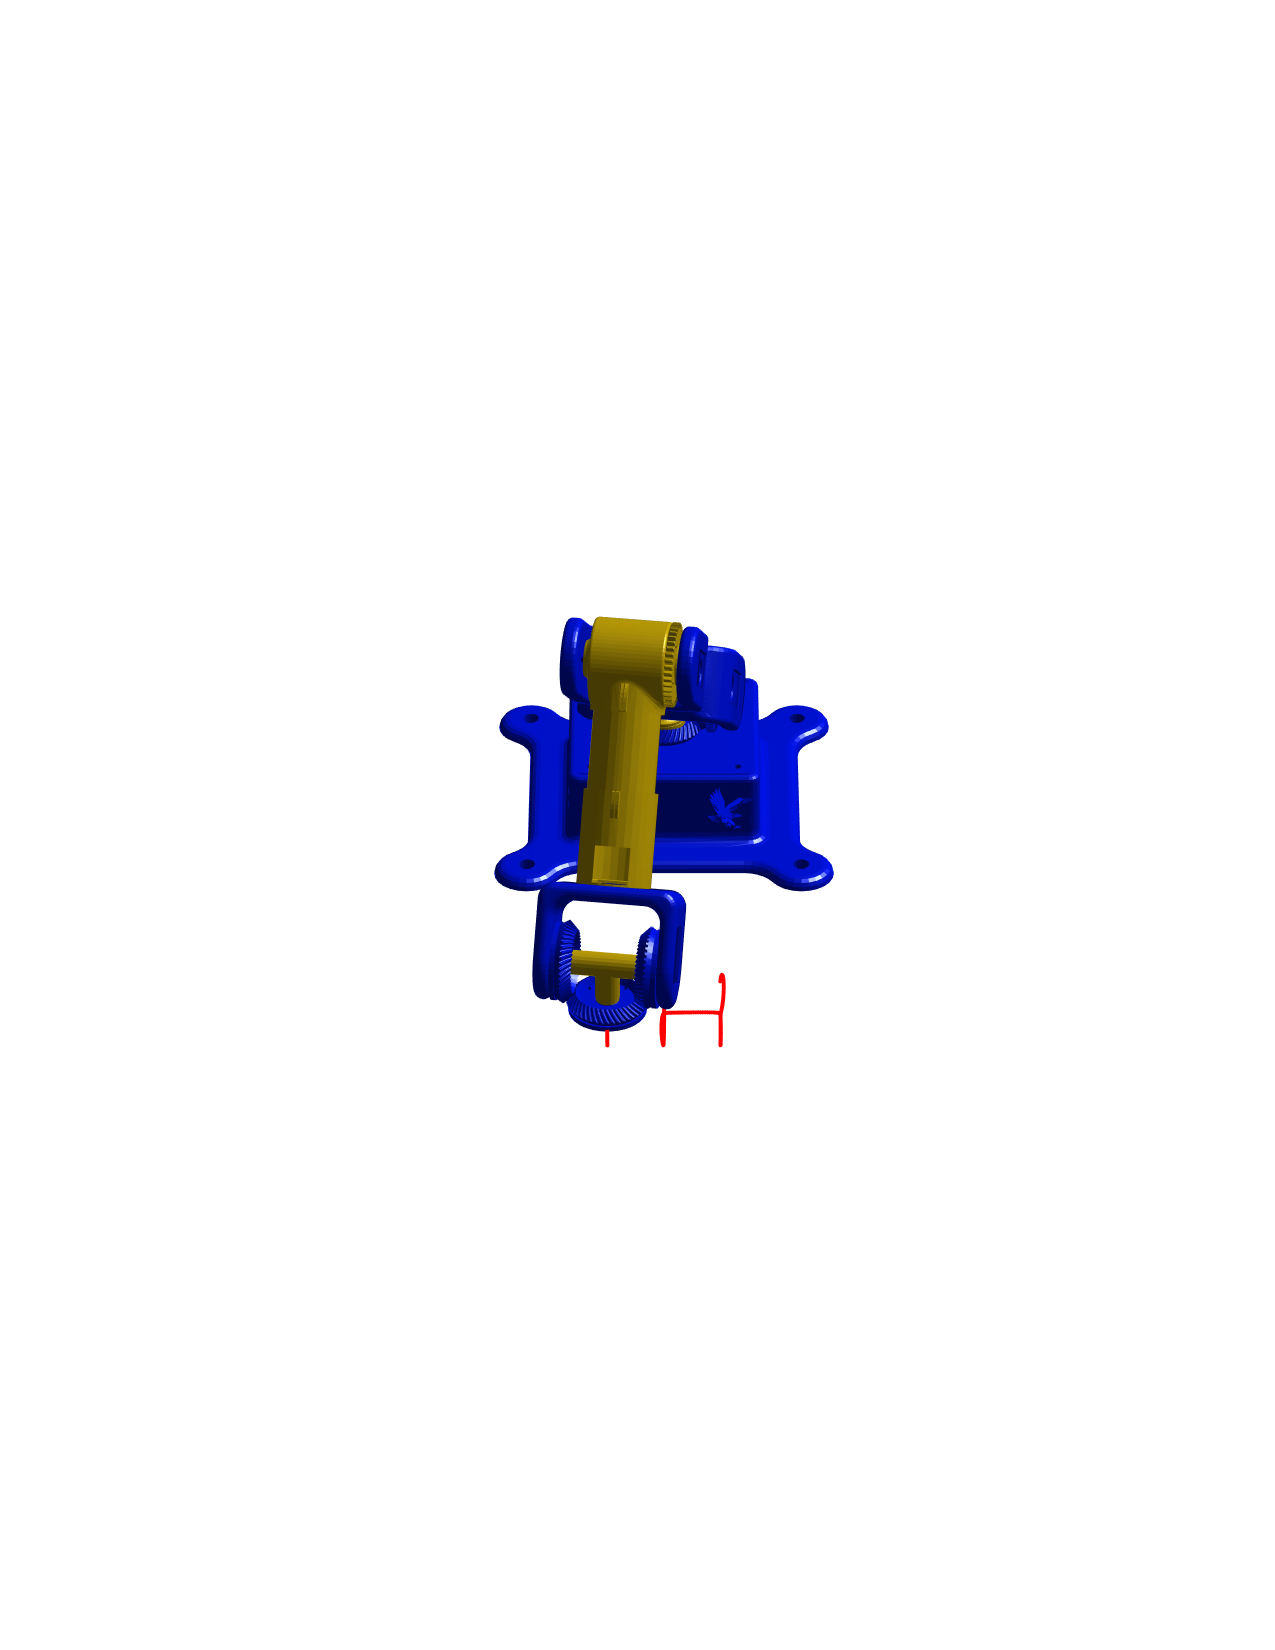
\includegraphics[width=.9\textwidth,frame]{clsnap3}
  \caption{Frame Snapshot near Simulation \\Termination}
\end{subfigure}
  \caption{Closed-Loop Control Simulation Animation Snapshots}
  \label{fig:clsnaps}
\end{figure}

\begin{figure}[htp]
  \center
  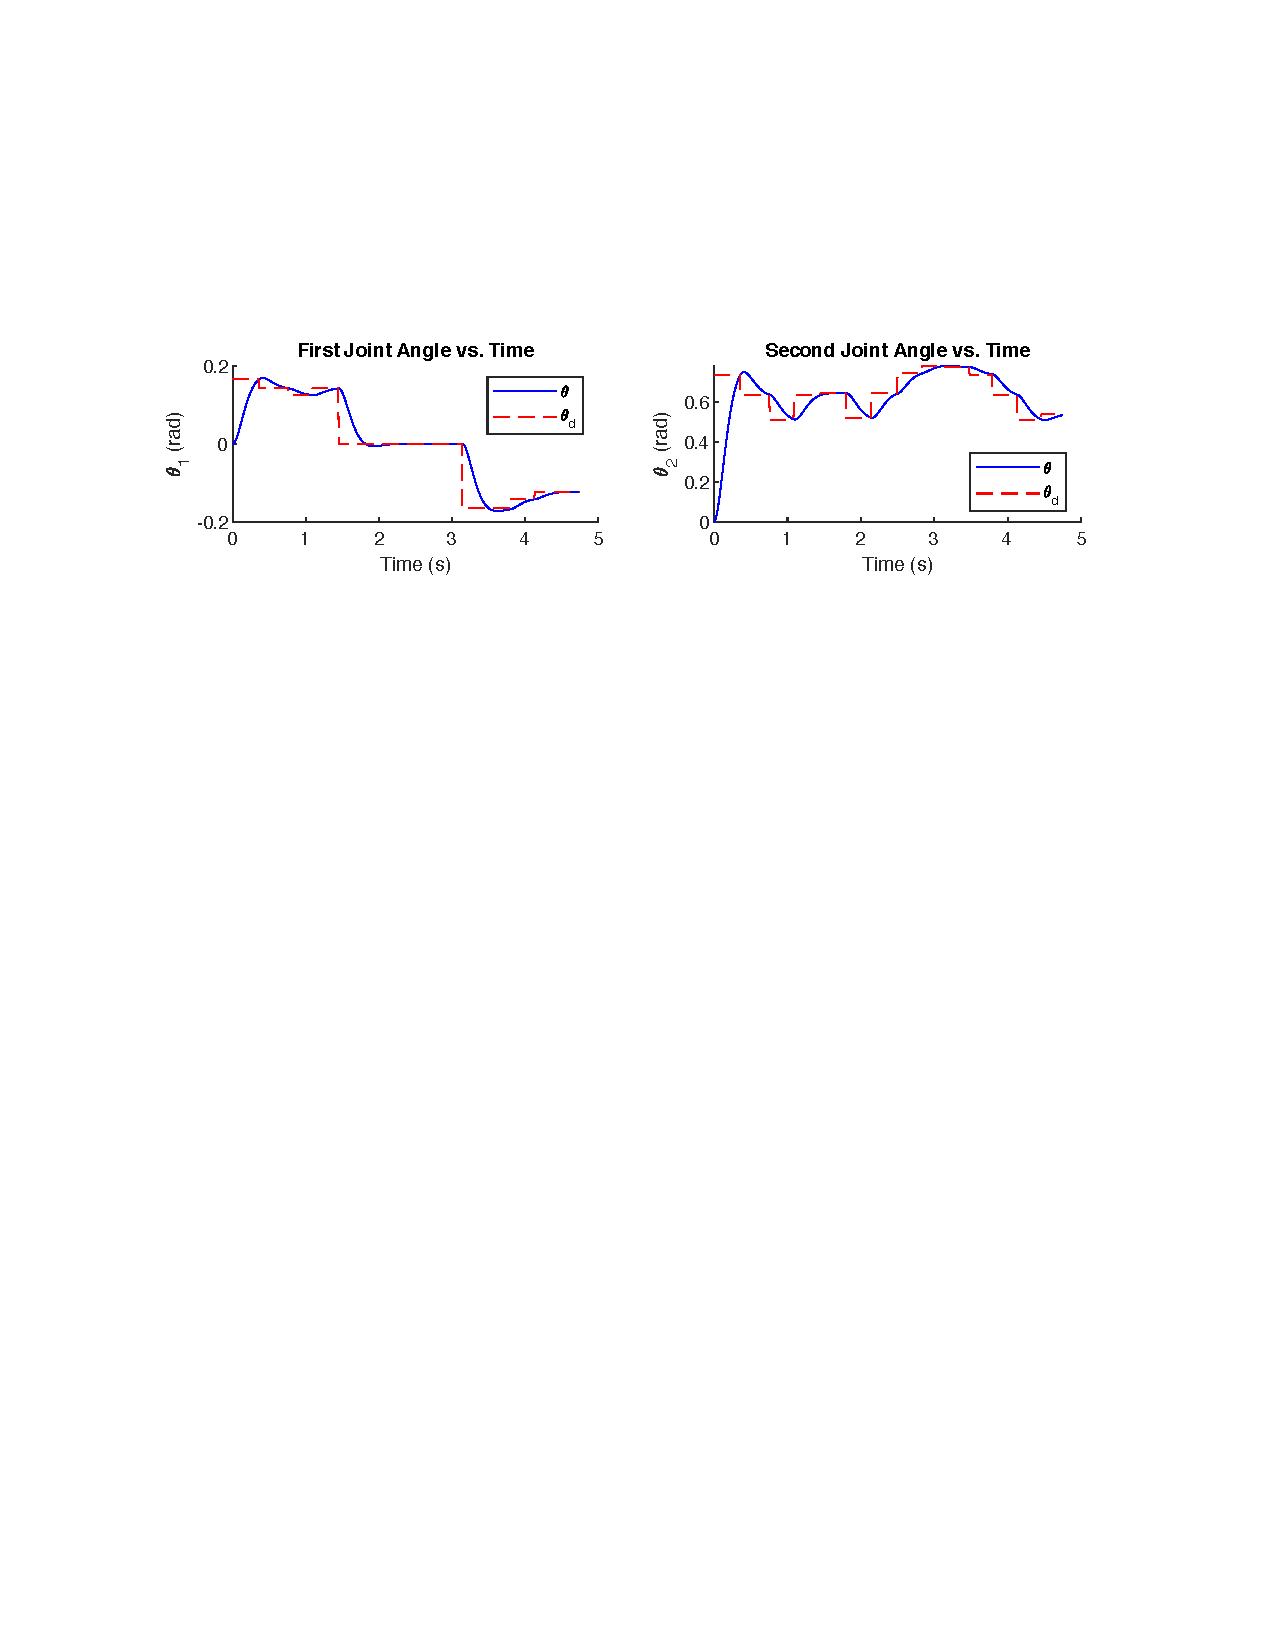
\includegraphics[width=.95\textwidth]{cljplots1}
  \caption{Joint Angles vs Time in Closed-Loop Simulation}
  \label{fig:cljplots1}
\end{figure}
\begin{figure}[htp]
  \center
  \ContinuedFloat
  \captionsetup{list=off,format=cont}
  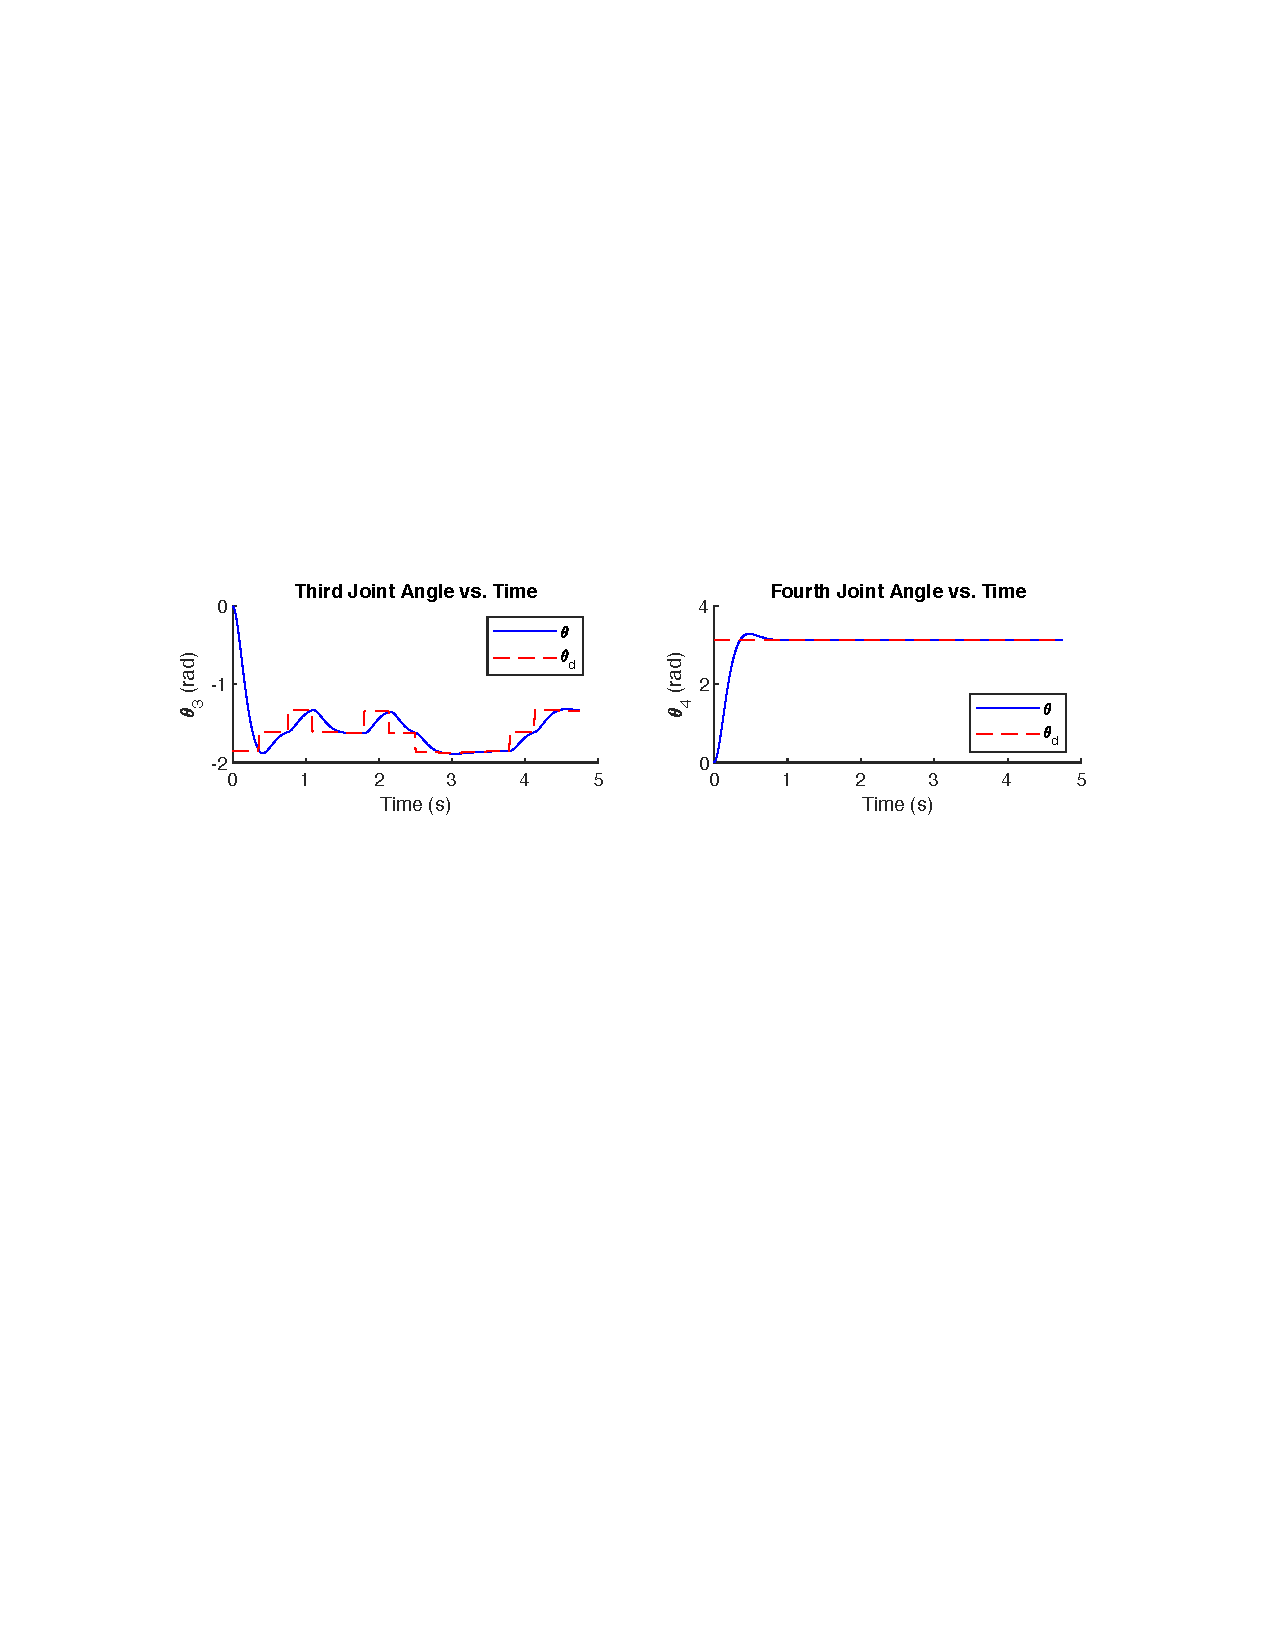
\includegraphics[width=.95\textwidth]{cljplots2}
  \caption{Joint Angles vs Time in Closed-Loop Simulation}
  \label{fig:cljplots2}
\end{figure}
\begin{figure}[htp]
  \center
  \ContinuedFloat
  \captionsetup{list=off,format=cont}
  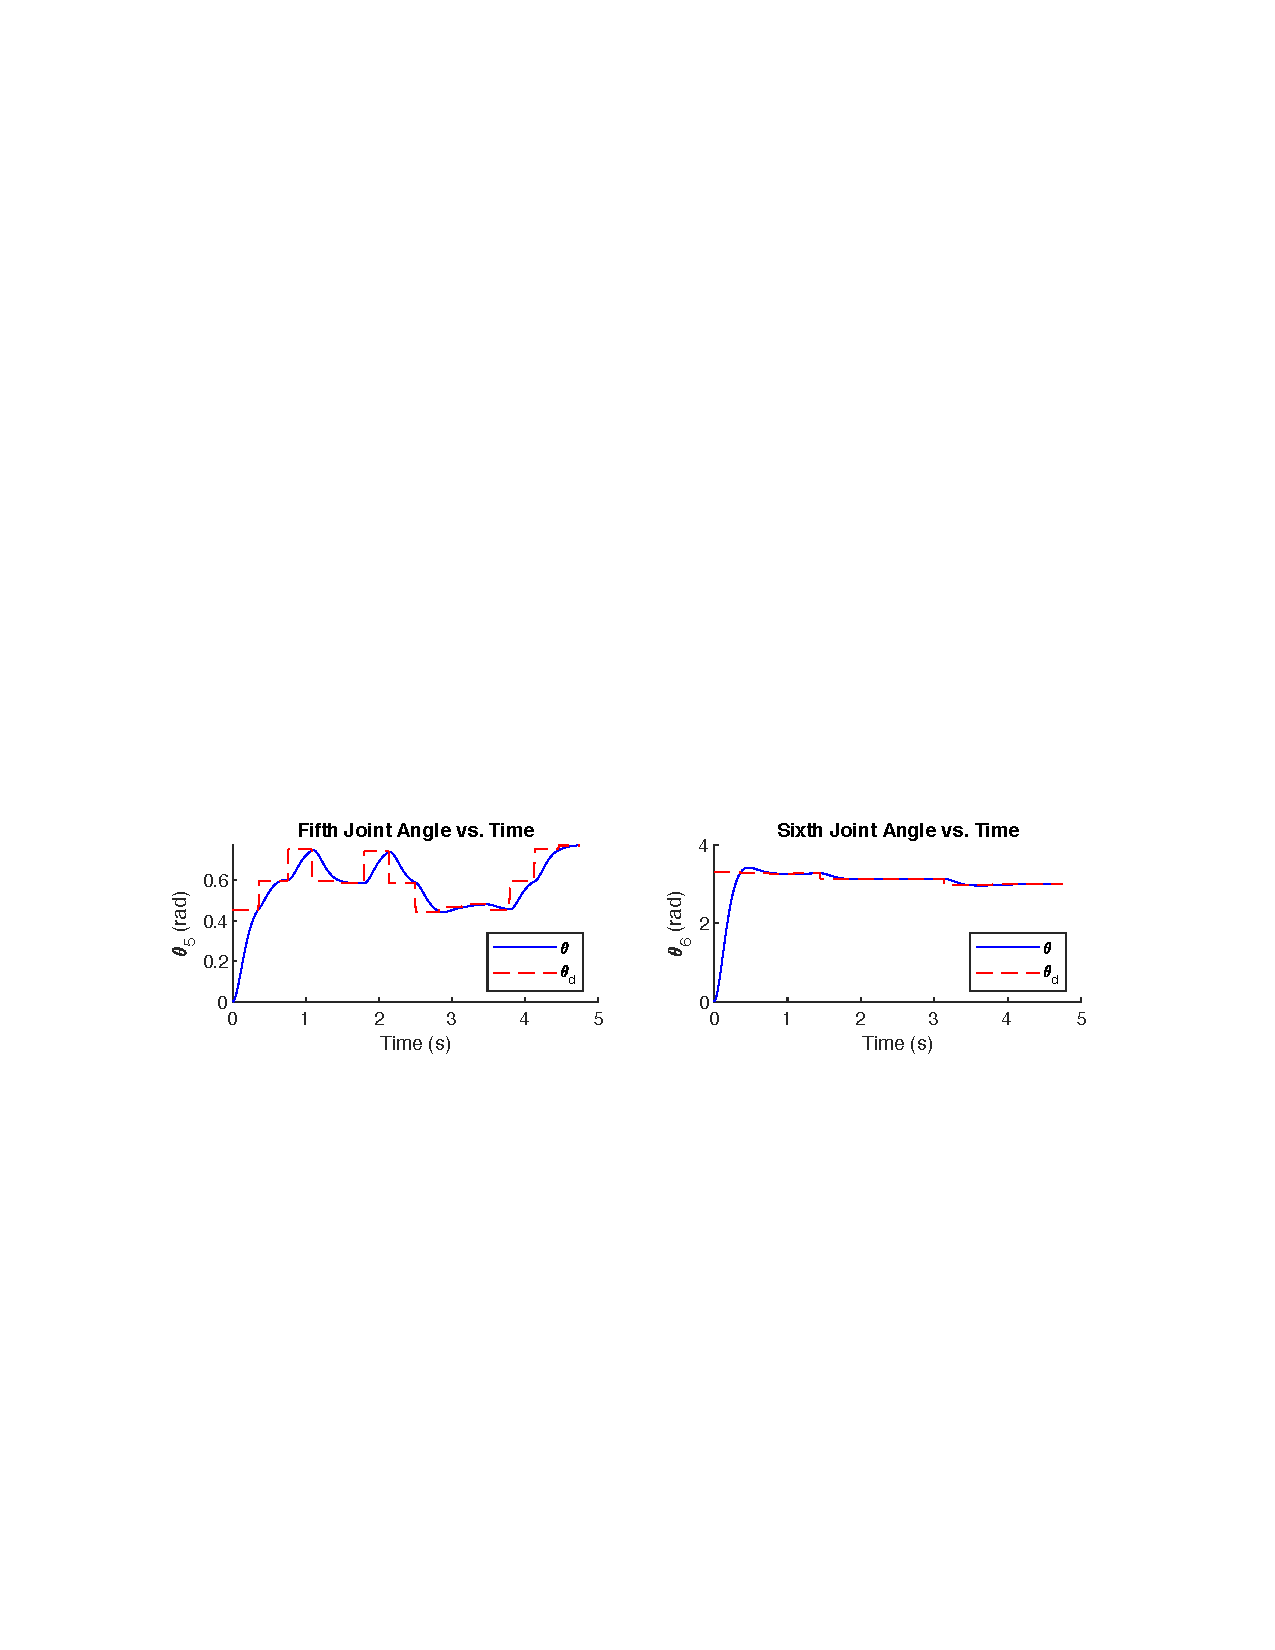
\includegraphics[width=.95\textwidth]{cljplots3}
  \caption{Joint Angles vs Time in Closed-Loop Simulation}
  \label{fig:cljplots3}
\end{figure}
\subsubsection*{ANSYS}
With 100\% infill, 3D printed PLA has a maximum shear stress of 13.6 kpsi. The manipulator applies a load of 13N in the negative y-direction. Without gears in the base differential, the differential support would bear the load on its bearing mounts. \emph{Figure \ref{fig:tbar}} shows the manipulator’s differential support could experience up to 97 kPa or 0.014 kpsi of shear stress, which is less than the maximum shear stress of PLA with 100\% infill. Since some of the manipulator’s mass is supported by the gears, the actual shear experienced by the differential support will be less.

\begin{figure}[htp]
  \center
  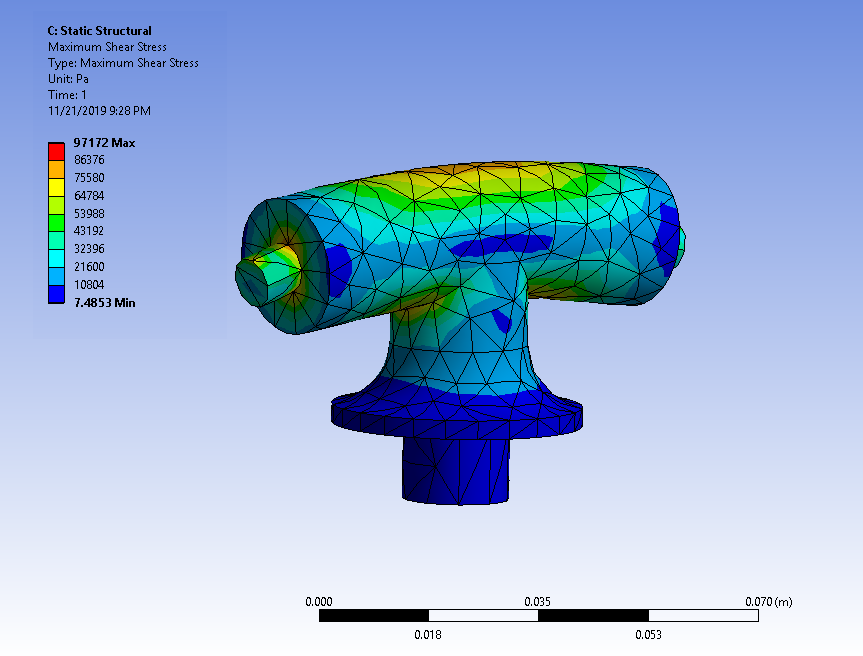
\includegraphics[width=.5\textwidth, frame]{tbar}
  \caption{T-Bar ANSYS FEA}
  \label{fig:tbar}
\end{figure}

To simulate a dynamical loading situation where the manipulator would be under the largest amount of stress, gravitational forces and an outward force (parallel to the arm direction in it's zeroed configuration) were applied to the structure. This situation represents the worst-case loading scenario, such as the manipulator swinging while outstretched. The supports and simulated forces can be seen in the ANSYS image capture shown in \emph{Figure \ref{fig:ansys_forces}}.
\begin{figure}[htp]
  \center
  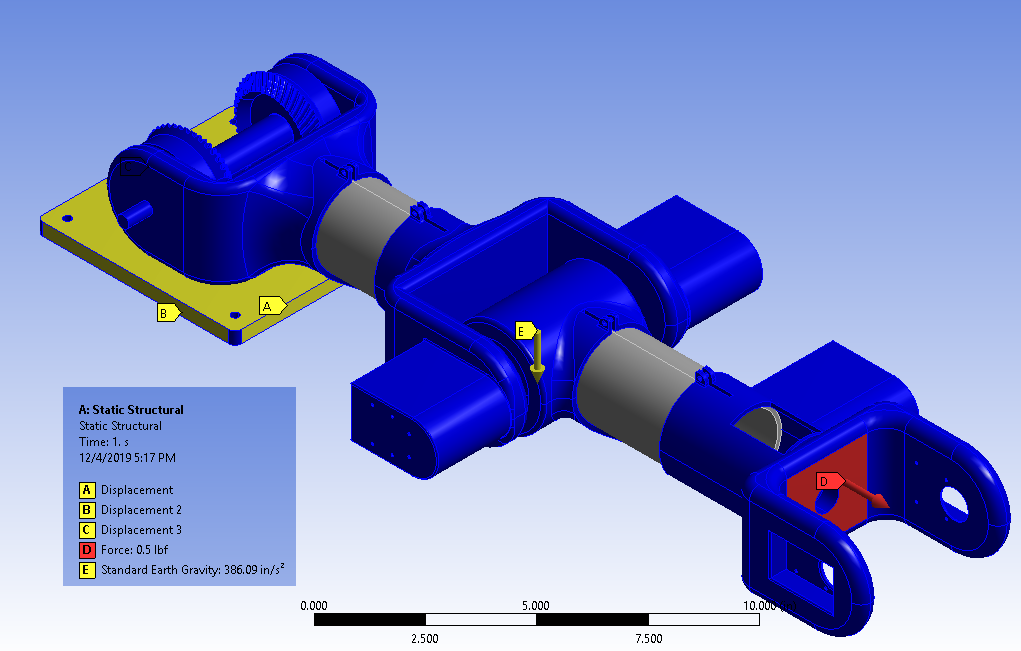
\includegraphics[width=.55\textwidth, frame]{ansys_forces}
  \caption{ANSYS Simulated Forces Image Capture}
  \label{fig:ansys_forces}
\end{figure}
\newpage
As shown in \emph{Figure \ref{fig:ansys_forces}}, the red arrow is the outward force simulating centrifugal forces, the yellow arrow represents gravity acting at the manipulator's center of mass, and the yellow highlighted faces show the fixed support at the base.

The dynamical loadings resulted in a maximum shear stress at the shoulder differential bearing, as seen in \emph{Figure \ref{fig:ansys_full}}; a close-up image of the bearing analysis can be seen in \emph{Figure \ref{fig:ansys_bearing}}.

\begin{figure}[htp]
  \center
  \begin{subfigure}[t]{0.5\textwidth}
  \center
  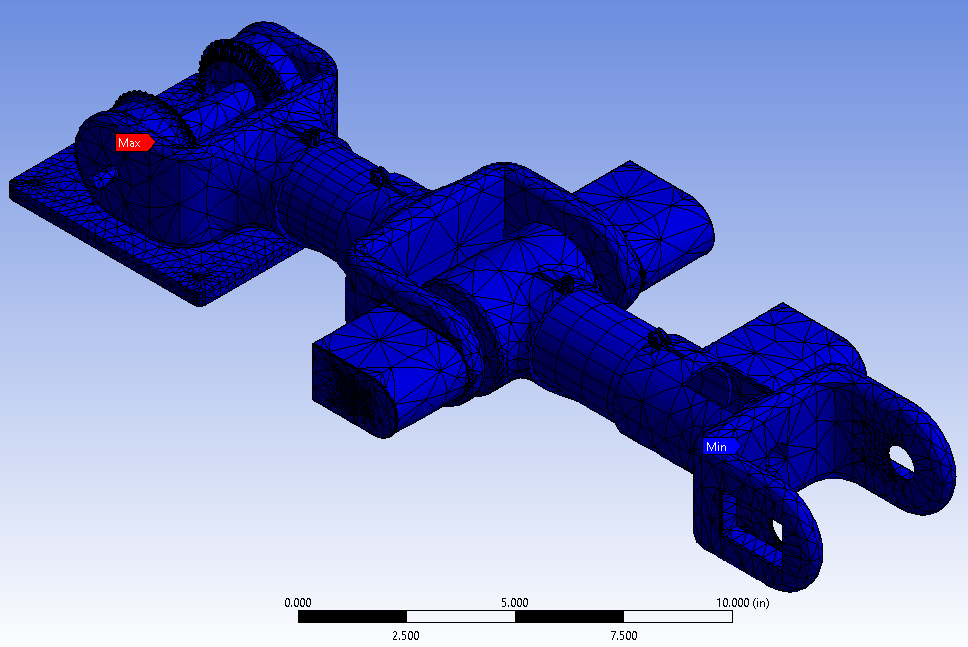
\includegraphics[width=.9\textwidth,frame]{ansys_full}
  \caption{ANSYS Full View of Maximum Shear}
  \label{fig:ansys_full}
\end{subfigure}%
\begin{subfigure}[t]{0.5\textwidth}
  \center
  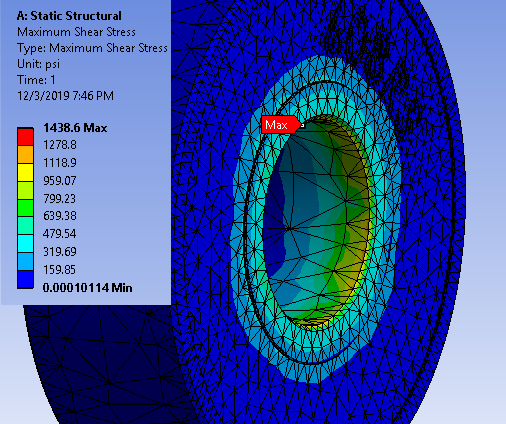
\includegraphics[width=.75\textwidth,frame]{ansys_bearing}
  \caption{ANSYS Bearing Shear Stress Close-up}
  \label{fig:ansys_bearing}
\end{subfigure}
  \caption{ANSYS FEA of Dynamical Loading Scenario}
\end{figure}

To further validate that the structure is capable of handling alternating stresses, a fatigue test was also performed showing the life of the manipulator handles a minimum of 1e6 cycles, as seen in \emph{Figure \ref{fig:ansys_life}}, showing it is unlikely to fail due to material yeilding.

\begin{figure}[htp]
  \center
  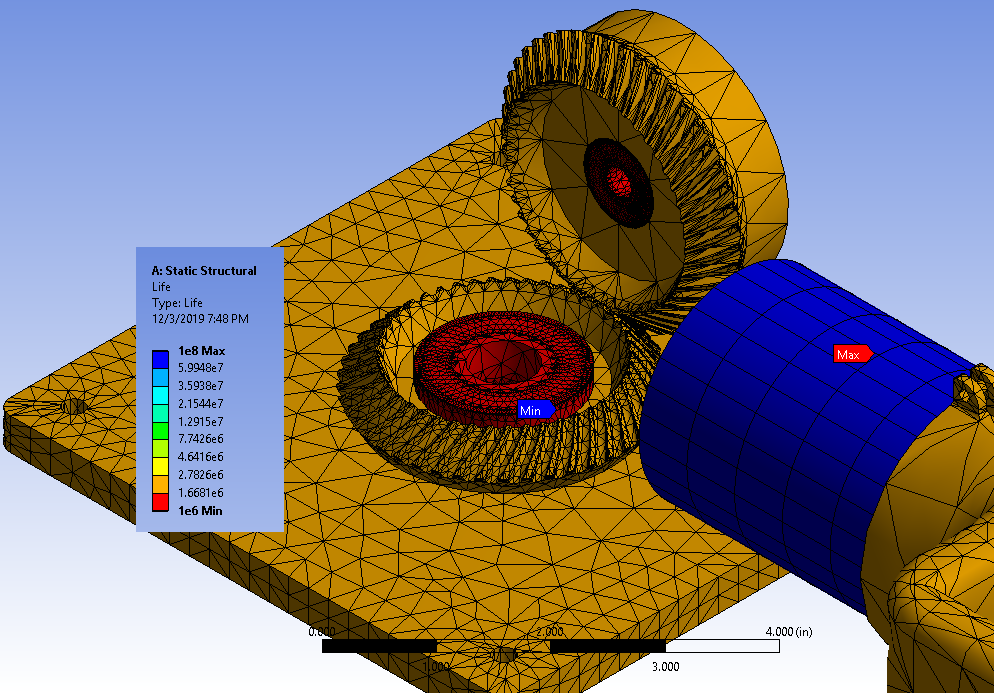
\includegraphics[width=.6\textwidth, frame]{ansys_life}
  \caption{ANSYS Fatigue Test}
  \label{fig:ansys_life}
\end{figure}

As seen in \emph{Figure \ref{fig:ansys_life}}, the lower bearing of the differential drive on the shoulder of the manipulator would be the most likely component to fail under repeating loadings.
\newpage
\subsection*{Parts list and budget}
\subsection*{Parts List}
\emph{Table \ref{tab:bom1}} lists the parts MEIOSIS will require to build the manipulator. The total cost is \$629.22, including shipping. Specification 1.1b requires MEIOSOS’s cost to develop the manipulator be less than \$800. In addition to pulley belts for the current configuration, \emph{Table \ref{tab:bom1}} allocates \$20 for two additional belt sizes to increase joint 1/2’s and joint 3’s torque by a factor of 10. The belts must be purchased in packs of 3 from Automation Direct and two more belt sizes may be required for the two pulley design to allow the servos to be mounted without interfering with the base. \emph{Table \ref{tab:bom1}} also accounts for increased cable lengths of 500 mm to communication bus signals from motor 2 to 3 and motor 3 to 4. And cable lengths of 350 mm to communication bus signals from motor 5 to 6. Motors are identified in [MOTOR ORIENTATION FIGURE]. Aside from electronic hardware, \emph{Table \ref{tab:bom2}} for physical hardware.
To allow screw mounting in plastic with metal threads, \emph{Table \ref{tab:bom2}} accounts for 100 threaded press-fit inserts. The manipulator will require between 21 and 46 inserts.The majority of inserts attach MX-12W servos to the manipulator. Mounting hardware accompanies each servo. Since purchasing six sets of pulleys would put MEIOSIS over the \$800 budget, they are printed.
\renewcommand{\arraystretch}{1.15}
\begin{table}[htp]
  \center
  \caption{MEIOSIS Bill of Materials with Costs}
  \label{tab:bom1}
\begin{tabular}{cC{3cm}@{\hskip 3pt}c@{\hskip 3pt}C{3cm}@{\hskip 3pt}|C{3cm}}
\multirow{2}{*}{\textbf{Part}} & \multirow{2}{*}{\textbf{Retailer}} & \multirow{2}{*}{\textbf{Quantity}} & \textbf{Unit Cost (USD)} & \textbf{Total Cost (USD)} \\\hline
3 pack, 300 tooth & \multirow{4}{*}{\shortstack[c]{Automation \\Direct}} & 1 & 11.5 & 11.5 \\
3 pack, 208 tooth &  & 1 & 9.5 & 28.5 \\
Base second belts &   & 1 & 10 & 10 \\
Link 3 second belts & & 1 & 10 & 10 \\\arrayrulecolor{gray}\hline
MX-12W & \multirow{4}{*}{\shortstack[c]{Trossen \\Robotics}} & 6 & 65.9 & 395.4 \\
500 mm, 1/2 pulleys &  & 2 & 3.95 & 7.9 \\
350 mm, 3 pulley &  & 1 & 2.95 & 2.95 \\
EE &  & 1 & 24.95 & 24.95 \\\arrayrulecolor{gray}\hline
Pi 3 B & \multirow{2}{*}{Amazon} & 1 & 37.99 & 37.99 \\
Bearings &  & 1 & 8.99 & 8.99 \\\arrayrulecolor{gray}\hline
\multirow{2}{*}{2 Sch 10 12" Al tube} & Industrial Metal Sales & 1 & 2.99 & 2.99 \\\arrayrulecolor{gray}\hline
\multirow{2}{*}{12 V, 5 V power supply} & Digi-Key Electronics & 1 & 43.21 & 43.21 \\\arrayrulecolor{gray}\hline
Automation Direct & \multirow{5}{*}{Shipping} & \multirow{5}{*}{---} & \multirow{5}{*}{---} & 0 \\
Trossen Robotics &  &  & & 13.15 \\
Amazon & &  & & 0 \\
Industrial Metal Sales &  & &  & 26.36 \\
Digi-Key &  & &  & 8.99 \\
& & & \textbf{Total} & 629.22 \\
\end{tabular}
\end{table}

In addition to the costs listed in \emph{Table \ref{tab:bom1}}, \emph{Table \ref{tab:bom2}} shows further costs for the end-user highlighted in blue. Since the Embry Riddle robotics lab has 3D printing available without affecting MEIOSIS’s \$800 budget, \emph{Table \ref{tab:bom2}} accounts for outsourced 3D printing costs sufficient to print the entire manipulator with six sets of pulleys. If the end-user owns a 3D printer, the 3D printing cost would effectively reduce to filament cost. Additionally, \emph{Table \ref{tab:bom2}} assumes the end-user does not already possess an AX-12A servo to be used with the end-effector. Further, \emph{Table \ref{tab:bom2}} assumes the manipulator would be more accessible to end-users by using a proprietary U2D2 communication module in lieu of a soldered or bread-board circuit.
The robotics lab has an AX-12A servo and U2D2 communication module MEIOSIS will use. With the aforementioned additional costs, the MEIOSIS manipulator costs the end-user  \$1,007.98 including shipping costs. While \$1,007.98 is slightly above the maximum cost of \$1000 from specification 1.1a, it provides greater accessibility, which may be diminished by assuming end-users poses 3D printers.

\renewcommand{\arraystretch}{1.25}
\begin{table}[htp]
  \center
  \caption{End-User Bill of Materials with Costs}
  \label{tab:bom2}
  \begin{tabular}{C{3cm}C{3cm}@{\hskip 3pt}c@{\hskip 3pt}C{3cm}@{\hskip 3pt}|C{3cm}}
  \multirow{2}{*}{\textbf{Part}} & \multirow{2}{*}{\textbf{Retailer}} & \multirow{2}{*}{\textbf{Quantity}} & \textbf{Unit Cost (USD)} & \textbf{Total Cost (USD)} \\\hline
  Aforementioned Costs & \multirow{2}{*}{\emph{Table \ref{tab:bom1}}} & \multirow{2}{*}{---} & \multirow{2}{*}{---} & 629.22 \\
  \multirow{2}{*}{U2D2} & Trossen Robotics & \multirow{2}{*}{1} & \multirow{2}{*}{49.9} & \multirow{2}{*}{49.9}\\
  \multirow{2}{*}{EE with servo} & Trossen Robotics & \multirow{2}{*}{1} & \multirow{2}{*}{64.95} & \multirow{2}{*}{64.95} \\
  3D PLA outsourcing (incl. shipping) & \multirow{2}{*}{Craft Cloud} & \multirow{2}{*}{1} & \multirow{2}{*}{288.86} & \multirow{2}{*}{288.86} \\
  & & & \textbf{Total} & 1007.98 \\
  \end{tabular}
\end{table}
\renewcommand{\arraystretch}{1}
\newpage

\section{Software}
\subsection*{Flowcharts}
The software the system will need will take in a row vector of position, orientation, path type, and end effector function information for all points to be traveled through and run the manipulator through the desired points following the specified paths requested. To do this, the user will first be asked what the number of points being input will be so that a few data structures can be preallocated. The user will then be asked if the manipulator will be writing or doing pick and place, and store the response. If the user is doing pick and place, the user will be asked for the full point data consisting of the x, y, and z location in millimeters, the phi, theta, and psi angles in degrees, the path type, and the end effector function. If the user is doing writing, only the x, y, and z locations will be requested. The orientation of the point will be defaulted in the “down” orientation since the marker will be held vertically, the path type will be set to cartesian straight line, and the end effector function will be set to stay unchanged. When all the desired points have been input, the software will then create intermediate points every centimeter between points whose paths are specified as cartesian straight line and store the new path points in a different data structure. After the path has been created, each point will be run through inverse kinematics to get the required joint angles to achieve the position and will be stored as the motor data for each point. If the user is writing with the manipulator, the user will be prompted to press a key to close the end effector to grab the marker. The user will then be prompted to press a key to begin, at which point the software will send the motor data to each servo for the first point that the system is trying to reach, wait till the servos are in the desired position, run the end effector function if there is one, and then repeat the process with the next set of motor data until all the points have been traveled through. When the last point has been reached, the program will prompt the user to input the number of desired points and wait for the input to start the process over again.
\captionsetup[sub]{
    labelformat=r-parens}
The software the system uses takes in a row vector of position, orientation, path type, and end effector function information for all points to be traveled through and runs the manipulator through the desired points following the specified paths requested. The general overview of the code is shown in \emph{Figure \ref{fig:soverall}}.

\begin{figure}[htp]
  \center
  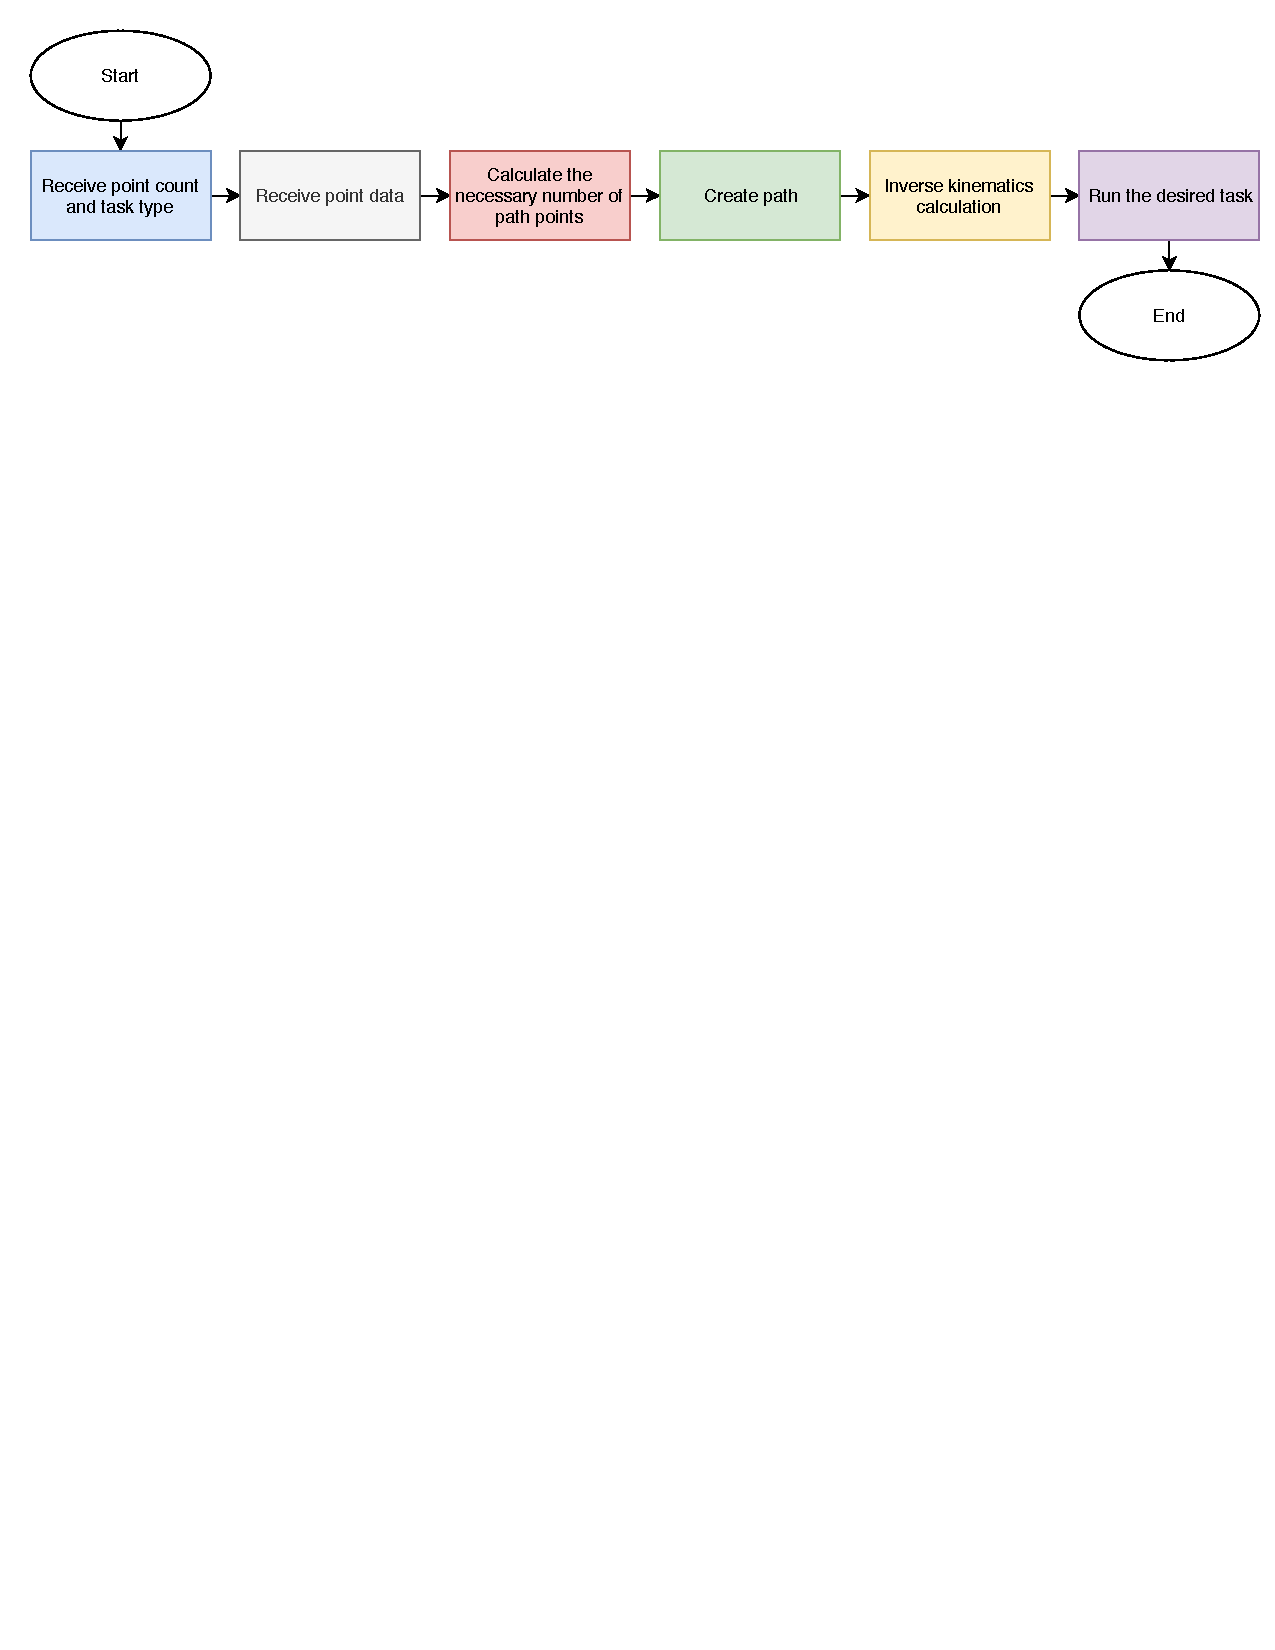
\includegraphics[width=\textwidth]{soverall}
  \caption{Software Flowchart}
  \label{fig:soverall}
\end{figure}

\emph{Figure \ref{fig:soverall}} shows that the software for the manipulator is broken up into six subsections, two sections that receive data, three that do calculations, and one that runs the specified task.

The first subsection of the software works to receive the number of points the user is inputting as well as the general task the user is completing, shown in \emph{Figure \ref{fig:sf1}}. \\

\begin{figure}[htp] \ContinuedFloat
  \begin{subfigure}[c]{\textwidth}
  \center
  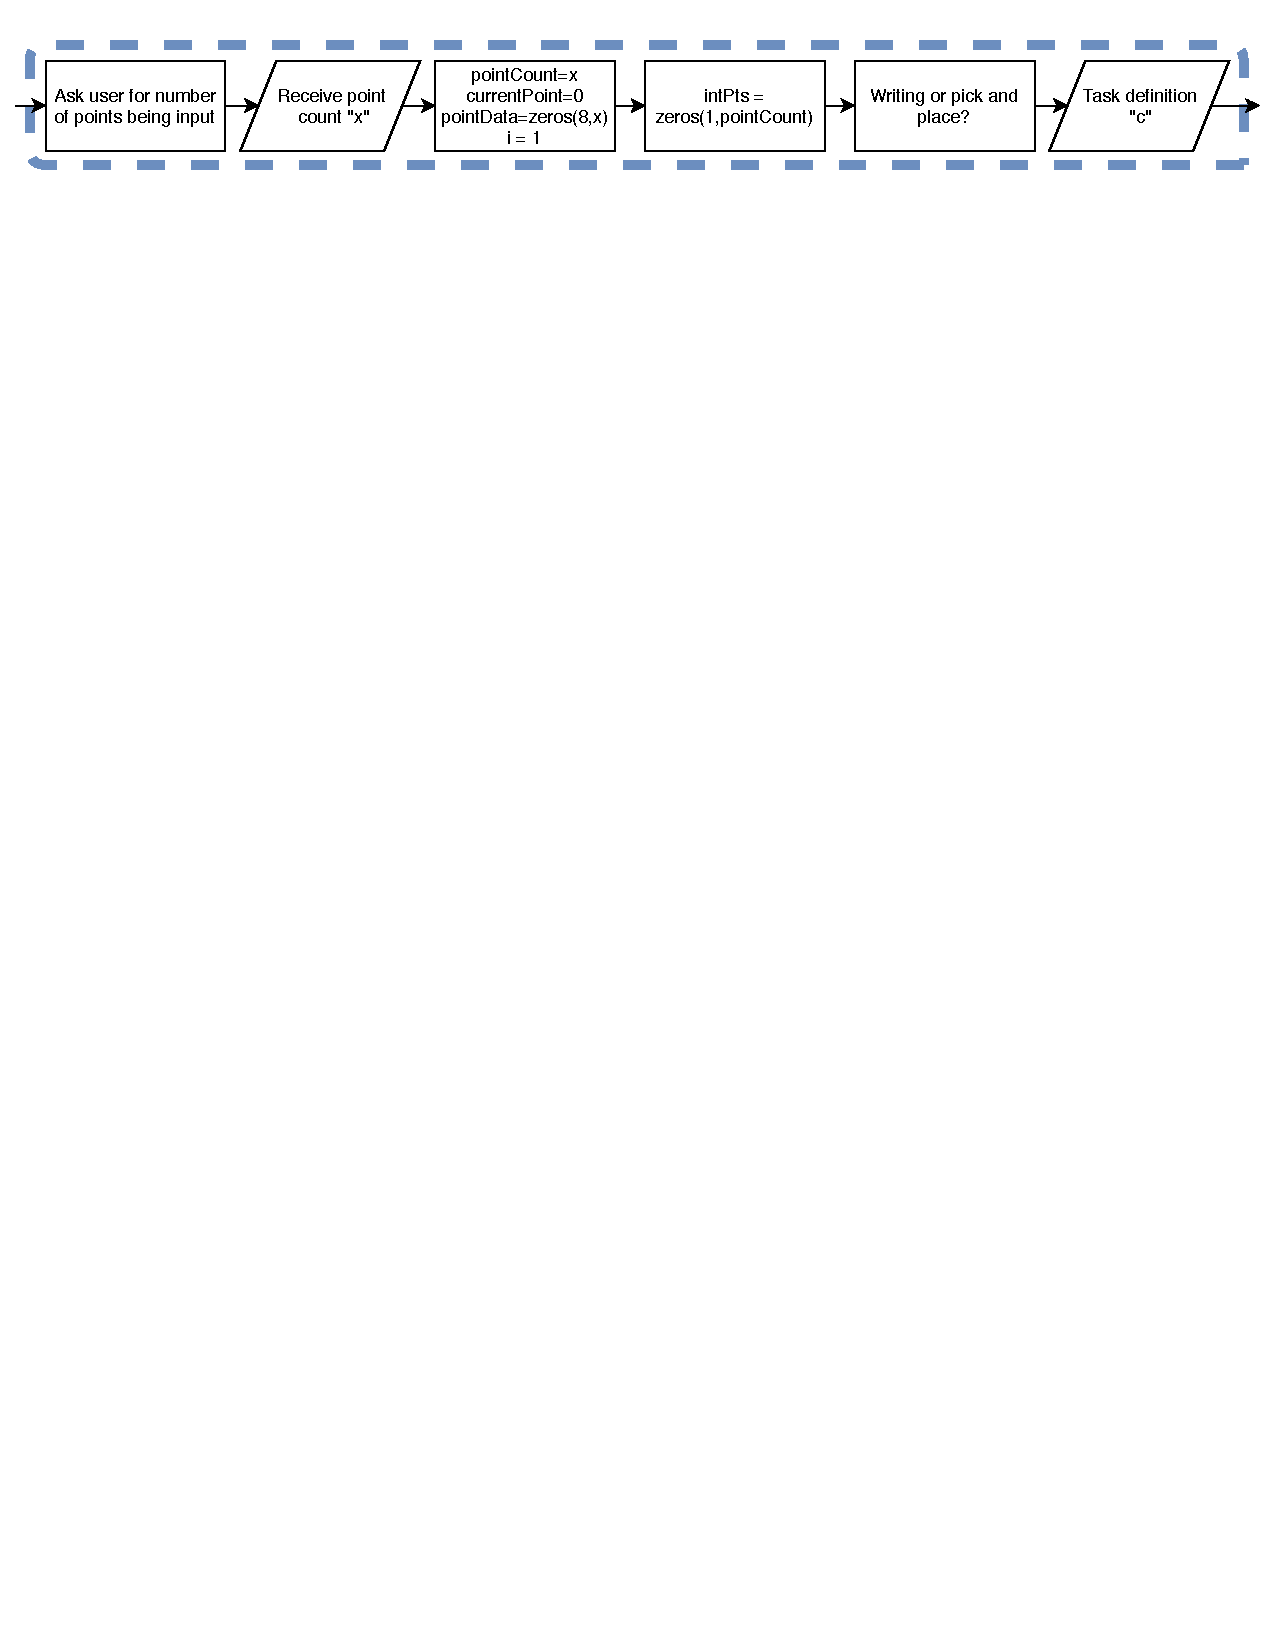
\includegraphics[width=\textwidth]{sf1}
  \caption{Software Flowchart Subsection 1}
  \label{fig:sf1}
  \end{subfigure}
\end{figure}

\emph{Figure \ref{fig:sf1}} specifies that the software prompts the user for the number of points that the manipulator will travel through and stores the input as a variable, in this case ‘x’. The ‘x’ variable is only used to help preallocate data vectors so that the size of the vector does not change with each input. The software also receives the task specification as either a 0 for cartesian straight line pathing or a 1 for a straight line in the joint space and stores this value in the variable ‘c’.

The second general block in the software flowchart works to receive and store the necessary data for the points the user is inputting depending on the path type as seen in \emph{Figure \ref{fig:sf2}}.
\begin{figure}[htp] \ContinuedFloat
  \begin{subfigure}[c]{\textwidth}
  \center
  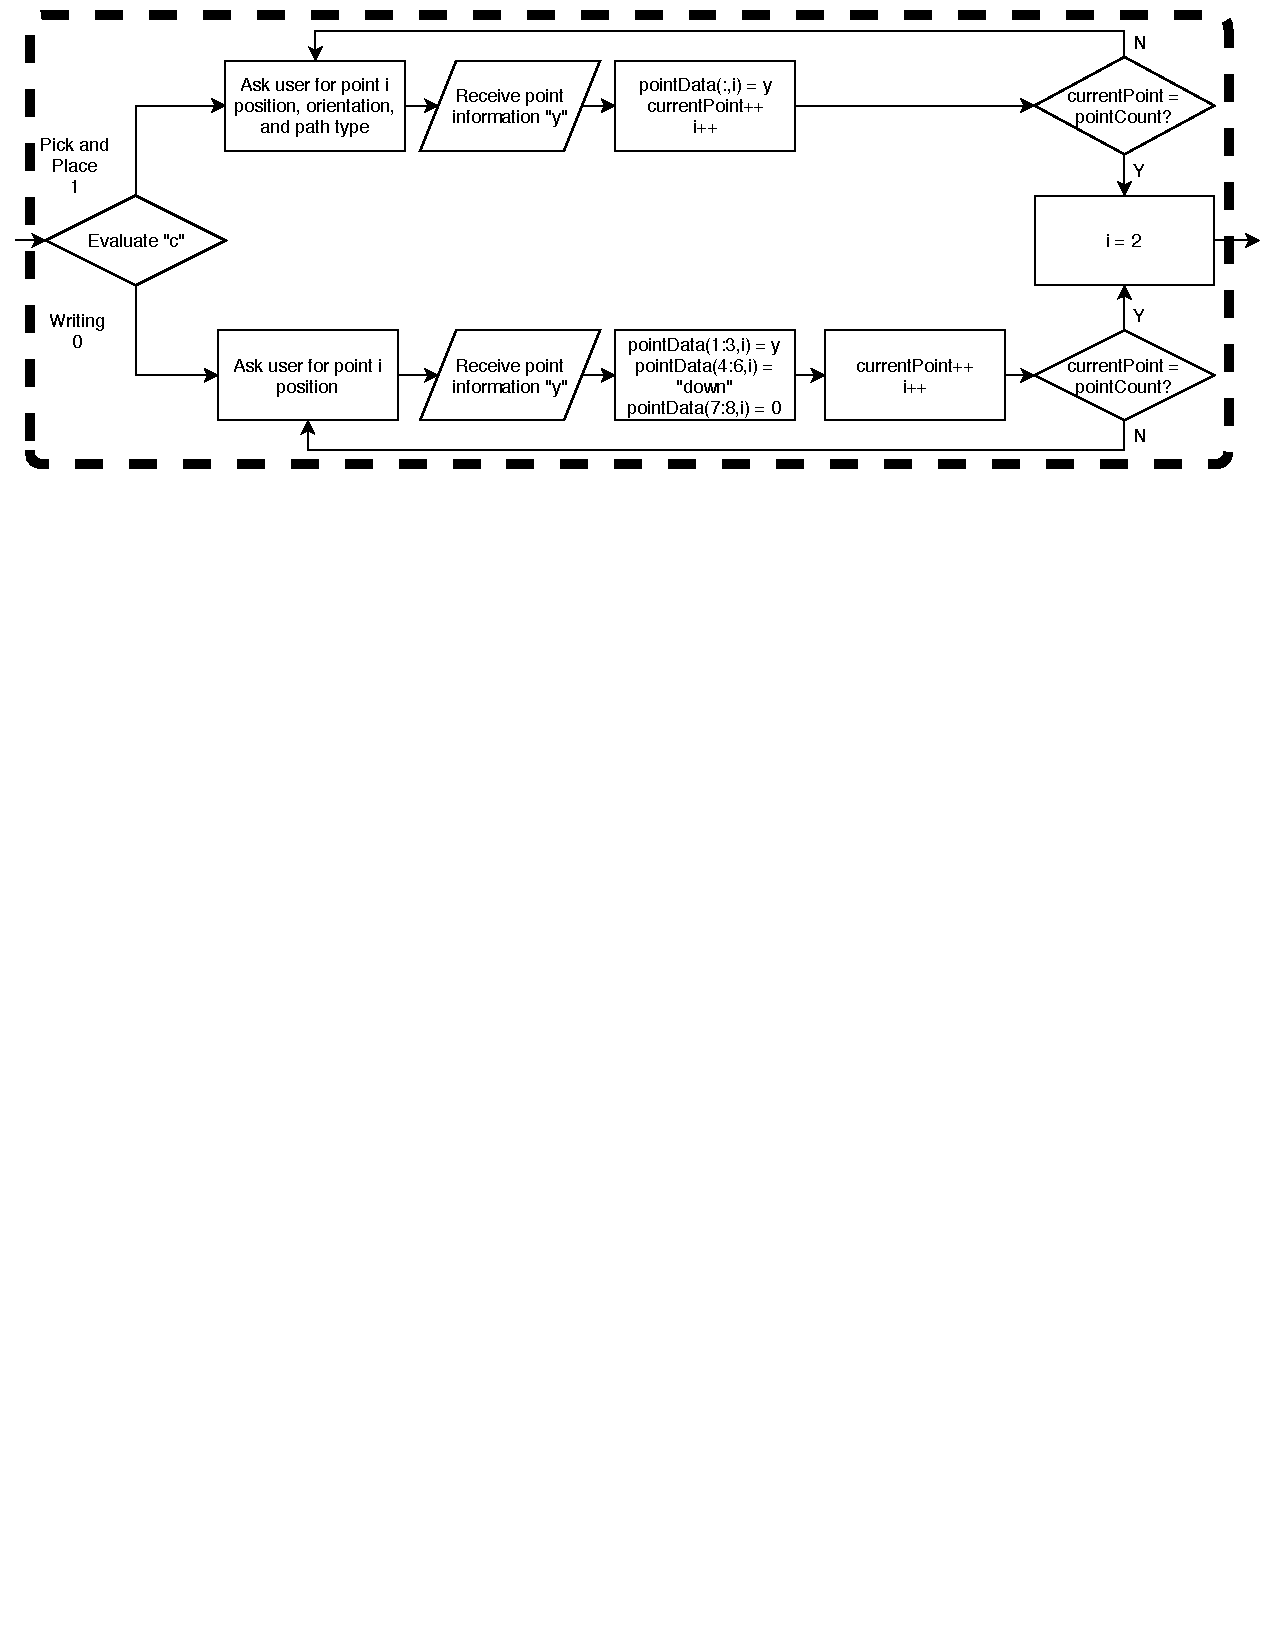
\includegraphics[width=\textwidth]{sf2}
  \caption{Software Flowchart Subsection 2}
  \label{fig:sf2}
\end{subfigure}
\end{figure}

\emph{Figure \ref{fig:sf2}} shows that the path type variable ‘c’ is used to determine what information is necessary to collect. If the user is doing a writing task, the software only collects the x, y, and z distances for the point and assumes that the end effector orientation will be facing down so that the marker is vertical. If the user is doing pick and place, the software prompts the user for the x, y, z, phi, theta, psi, path type, and end effector data. The software loops until all the points have been input.

The next block in the software flowchart calculates the total points necessary to complete the task. The overview for this section can be seen in \emph{Figure \ref{fig:sf3}}.

\begin{figure}[htp]\ContinuedFloat
  \begin{subfigure}[c]{\textwidth}
  \center
  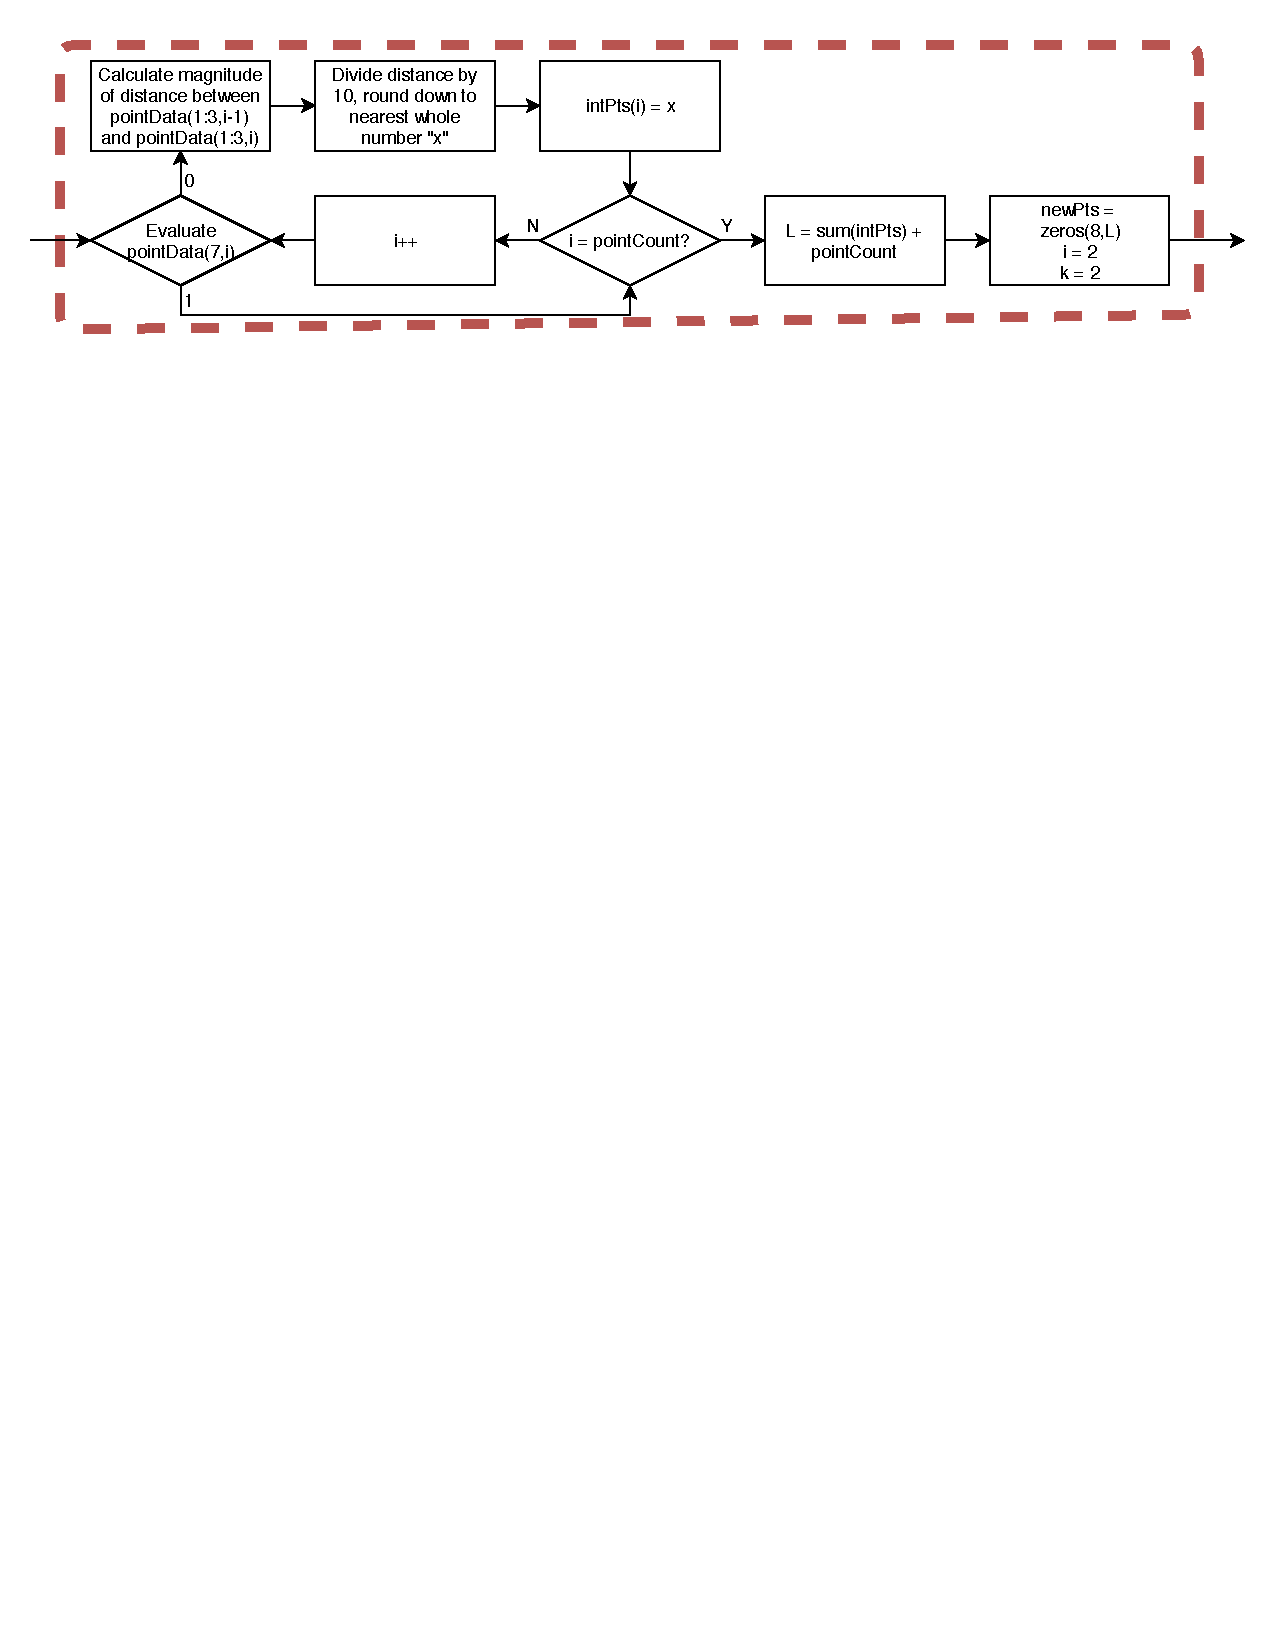
\includegraphics[width=\textwidth]{sf3}
  \caption{Software Flowchart Subsection 3}
  \label{fig:sf3}
  \end{subfigure}
\end{figure}

As seen in \emph{Figure \ref{fig:sf3}}, the section of software calculates the distance between the current point and the previous point if the path type is cartesian straight line and divides the distance by ten to find the number of centimeters between the two points. This value is stored as the necessary number of intermediate points, and the software will loop through until every point has been checked. The section of code also stores the total number of points that will be used as the variable level for later use.
\newpage
The fourth code block in the flowchart creates and stores the necessary intermediate points along the desired path, shown in \emph{Figure \ref{fig:sf4}}.

\begin{figure}[htp] \ContinuedFloat
  \begin{subfigure}[c]{\textwidth}
  \center
  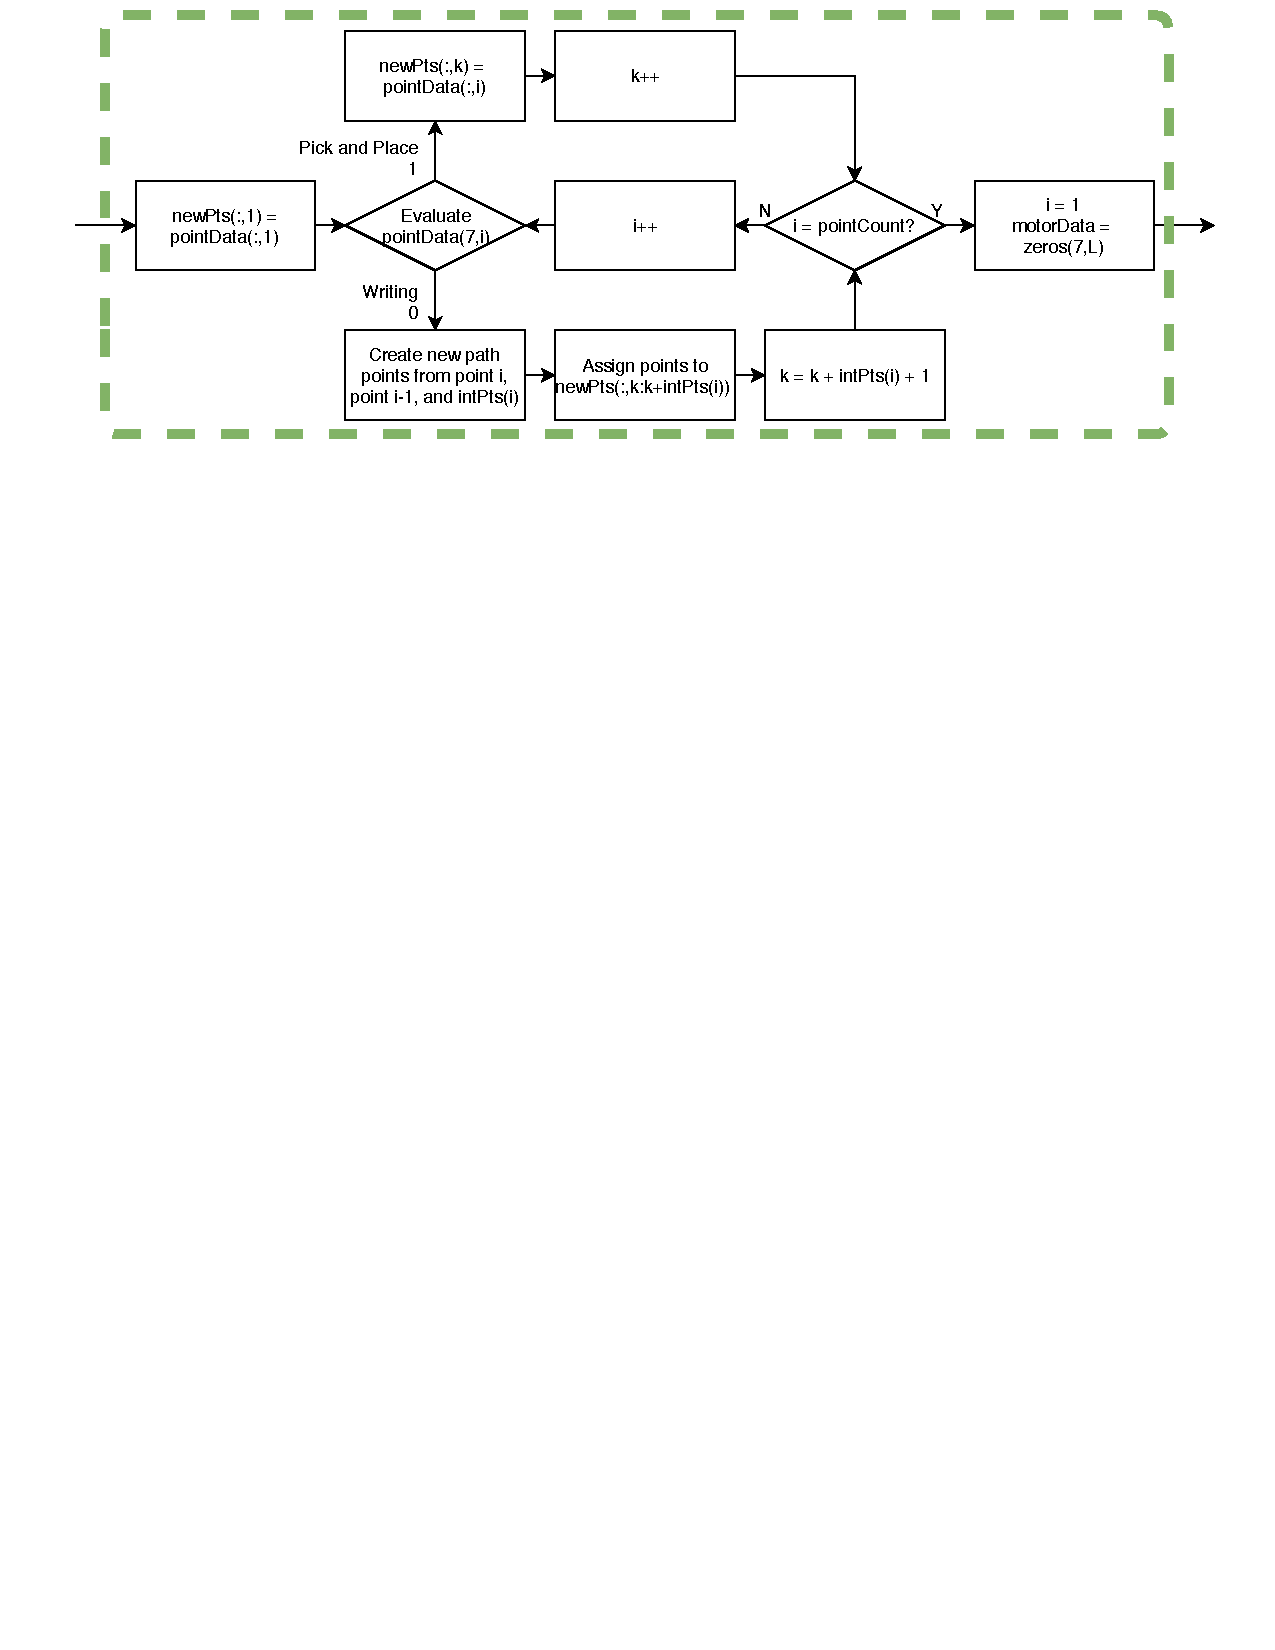
\includegraphics[width=.99\textwidth]{sf4}
  \caption{Software Flowchart Subsection 4}
  \label{fig:sf4}
  \end{subfigure}
\end{figure}
\looseness=-1

The code shown in \emph{Figure \ref{fig:sf4}} creates points every centimeter if the path type is cartesian straight line using the number of path points stored for each point from the previous block of software. This ensures that a straight line will be followed between the two user input points. If the path type is a straight line in the joint space, the software does not add any intermediate points since the path seen in the cartesian space does not matter.

The fifth code block in the flowchart calculates inverse kinematics of the points defined in the previous block of code and stores the angles as counts that can be used by the servos. The overview of this section can be seen in \emph{Figure \ref{fig:sf5}}.

\begin{figure}[htp] \ContinuedFloat
  \begin{subfigure}[c]{\textwidth}
  \center
  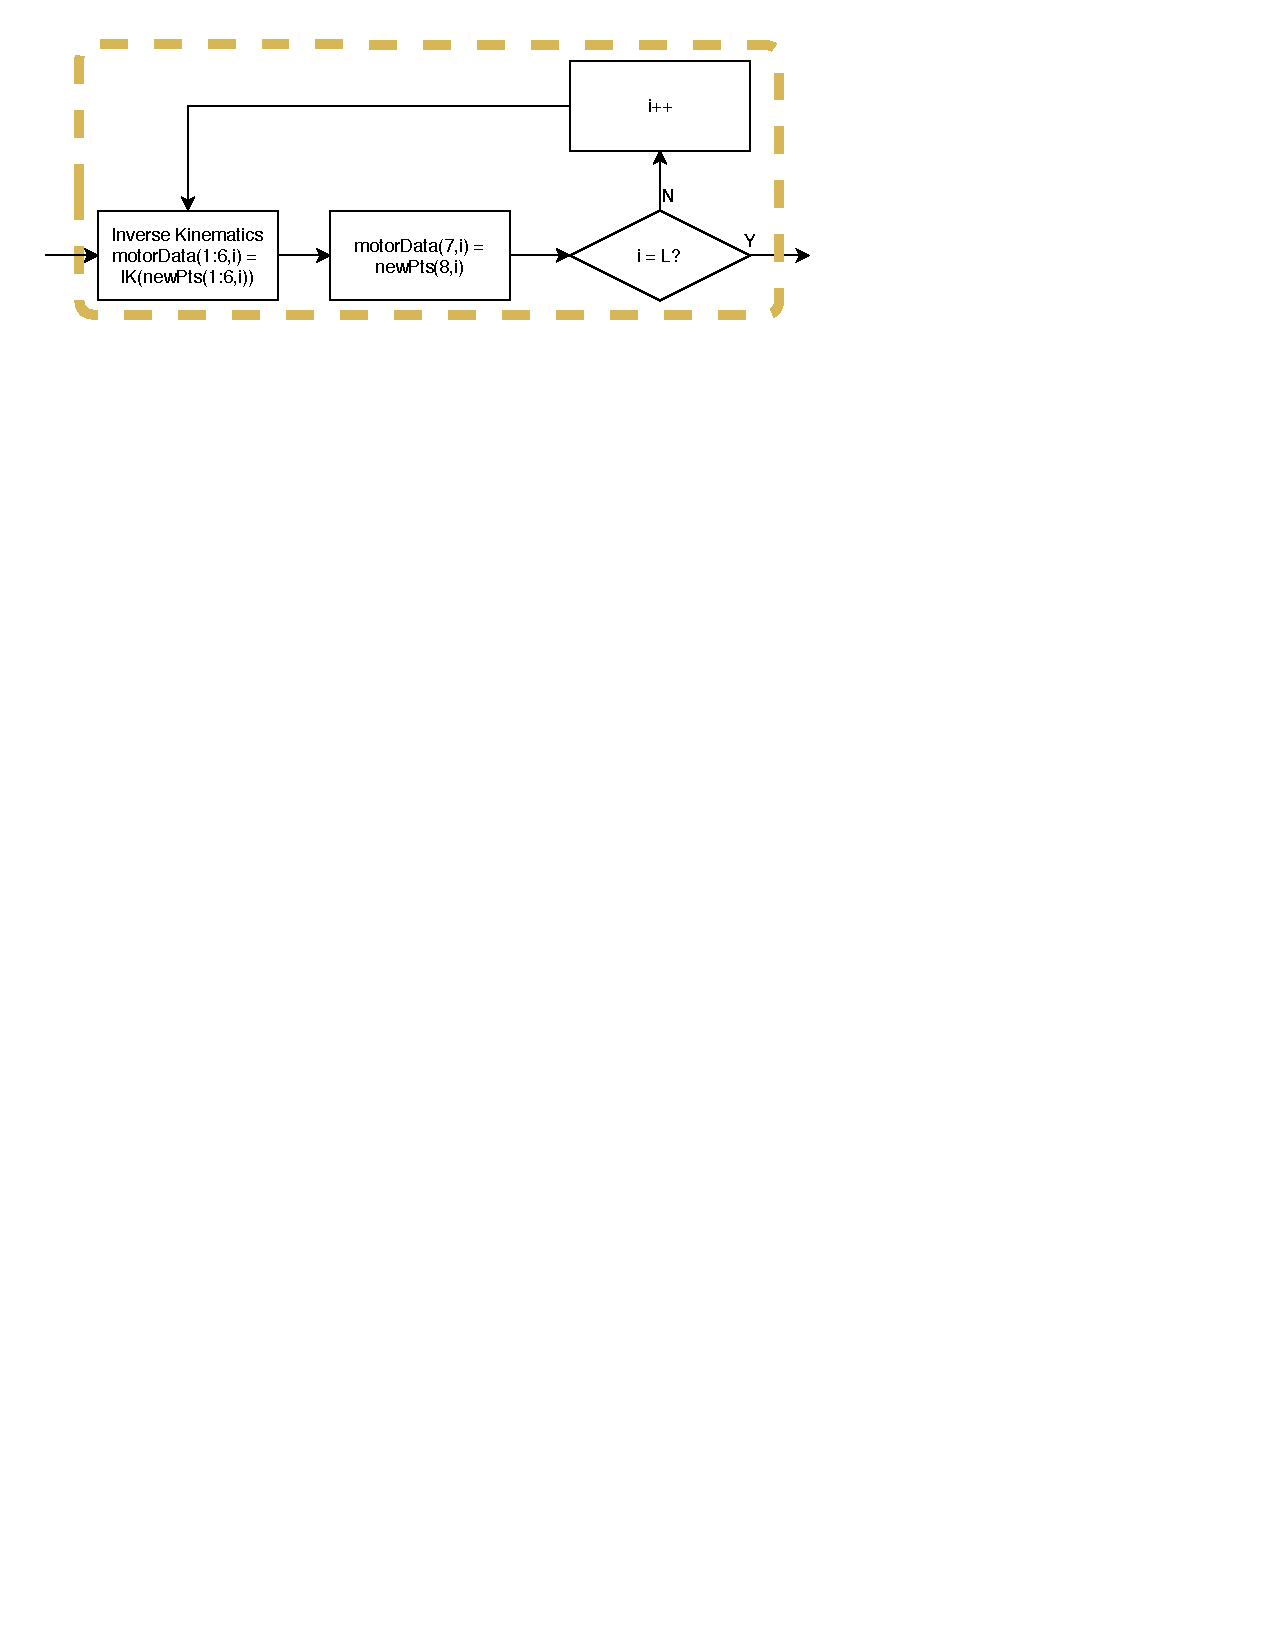
\includegraphics[width=\textwidth]{sf5}
  \caption{Software Flowchart Subsection 5}
  \label{fig:sf5}
  \end{subfigure}
\end{figure}

\emph{Figure \ref{fig:sf5}} shows that the new points found in the prior section of code are run through an inverse kinematics function that will output the necessary counts the servos can utilize. The code iterates through each point until the inverse kinematics have been calculated for all points.

The final block in the software diagram runs the manipulator through the desired task, with this section of code requiring user input at certain stages depending on the path type, seen in \emph{Figure \ref{fig:sf6}}.
\begin{figure}[htp] \ContinuedFloat
  \begin{subfigure}[c]{\textwidth}
  \center
  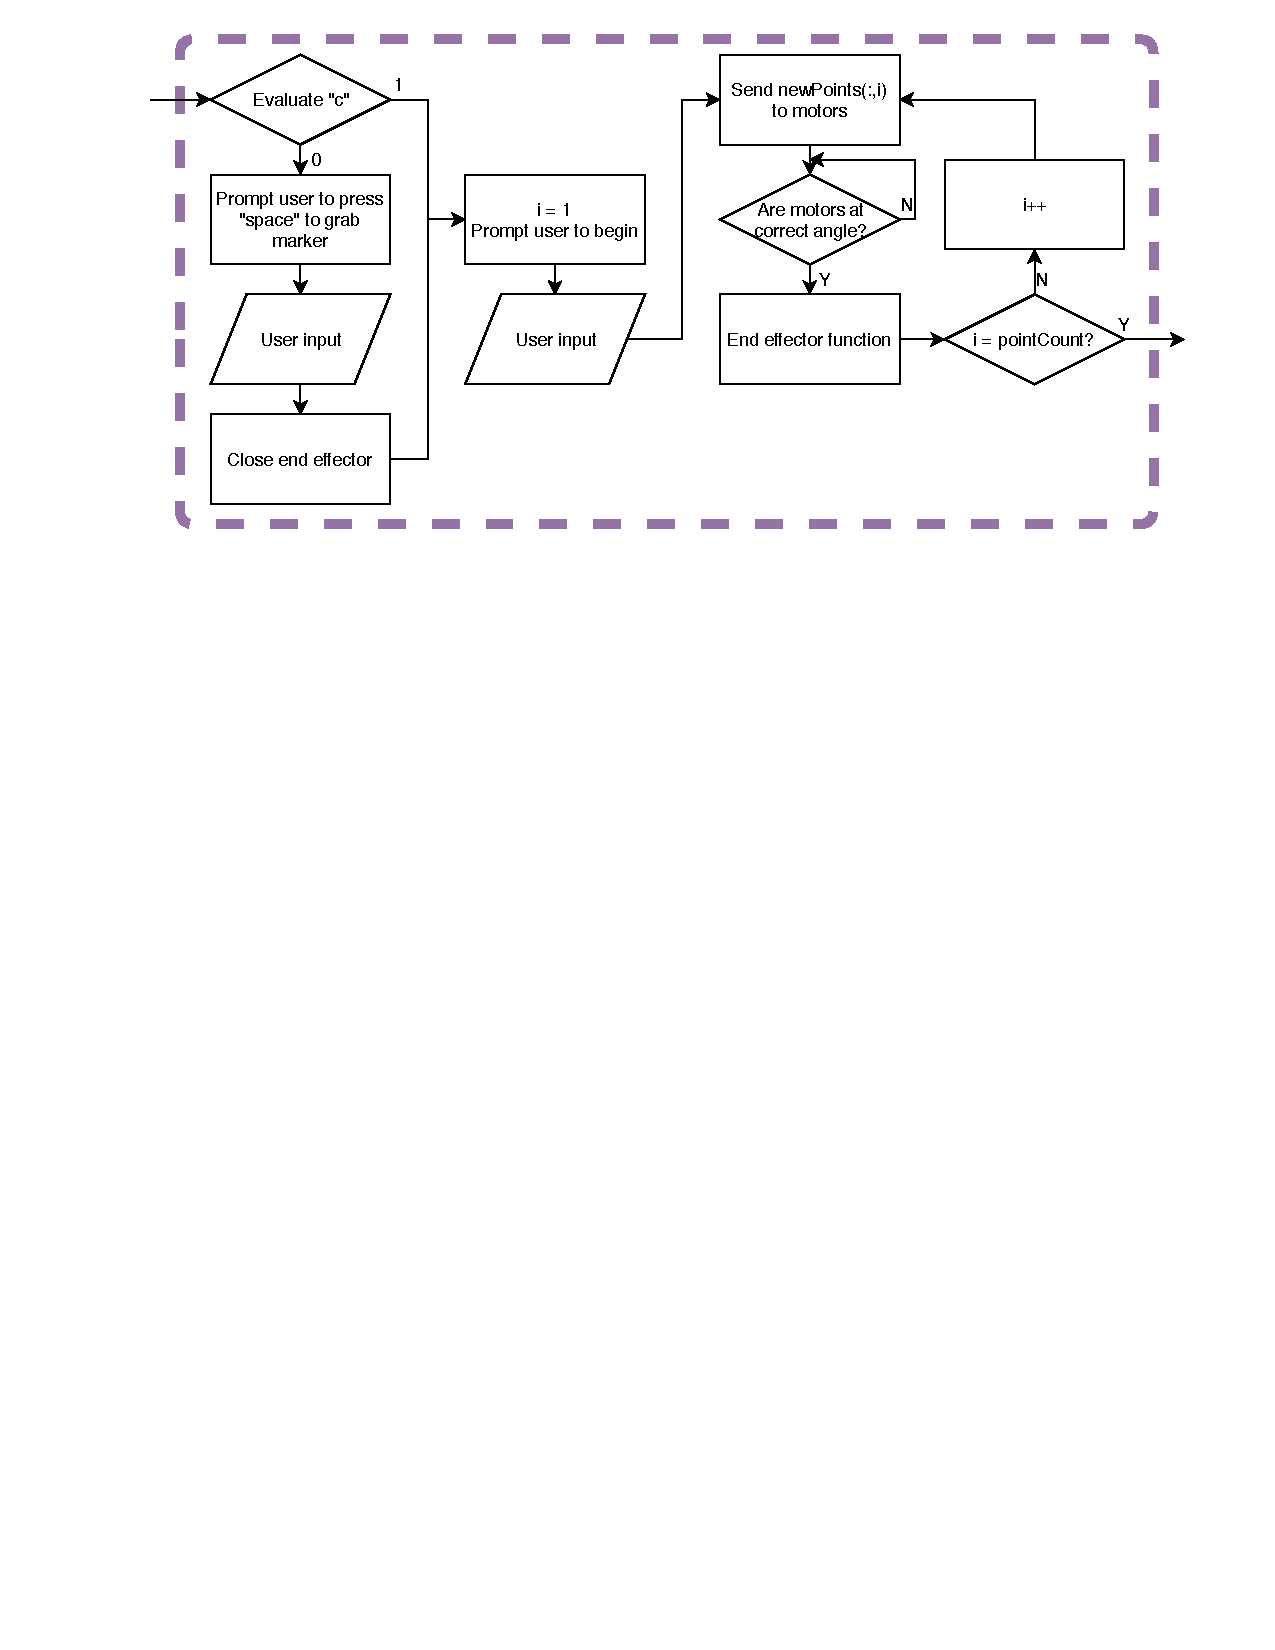
\includegraphics[width=\textwidth]{sf6}
  \caption{Software Flowchart Subsection 6}
  \label{fig:sf6}
  \end{subfigure}
\end{figure}

The code in \emph{Figure \ref{fig:sf6}} prompts the user to press space to close the end effector and grab the marker if drawing was the specified task, otherwise the software jumps straight into prompting the user to begin the task, and when the user begins the task the counts for each position are sent to the servos one at a time. The counts for the next position are not sent to the servos until the servos have reached the desired positions and the end effector function has been completed if there is one.

\subsection*{Description of control system}
\subsection*{Implementation}
The implementation of the software control algorithm described in the software flowcharts was not able to be finished to completion, although the basic control scheme of the manipulator was established with Python scripts. The MATLAB code written for simulation of the manipulator, such as the inverse kinematics calculations, were converted to Python and successfully implemented. Since only two joints of the manipulator were written, a two link inverse kinematics function was implemented as well as servo control algorithms to ease future programming. Snippets of the servo control scheme as well as the two link arm inverse kinematics can be seen in Listings \ref{code:pyik} \& \ref{code:pyservo}.

\begin{lstlisting}[frame=line,language=Python,label=code:pyik,caption=twolink.py]
def twoLinkIK(x,y):
    l1 = 265.0
    l2 = 165.0
    D = (x**2 + y**2 - l1**2 - l2**2)/(2*l1*l2)
    theta2 = atan2(sqrt(1.0 - D**2),D)
    theta1 = atan2(y,x) - atan2(l2*sin(theta2),l1+l2*cos(theta2))
    print(degrees(theta1),degrees(theta2))
    return [degrees(theta1),degrees(theta2)]
\end{lstlisting}
The \texttt{meiosis\_servo.py} file contains several methods composed in an attempt to simplify and expedite future programming.
\begin{lstlisting}[frame=line,language=Python,label=code:pyservo,caption=meiosis\_servo.py]
#!/usr/bin/env python
# -*- coding: utf-8 -*-

"""basic readable servo commands"""

from dynamixel_sdk import *
...
def setJA(self, IDLIST, angle):
  if(type(IDLIST) == int):
      IDLIST = [IDLIST]
  if(type(angle) == int):
      angle = [angle]
  for i in range(0,len(IDLIST)):
      self.setPos(IDLIST[i], int(round(angle[i] * gearidx[i]...
         + offset[i])))
      print(int(round(angle[i] * gearidx[i] + offset[i])))
\end{lstlisting}
The \texttt{setJA} method shown above is an example of how a basic function needed for future programming was methodically created in an attempt to ease the burden of the final manipulator implementation. All methods were created with versatility in mind; the testing performed was limited to a two link manipulator since that is all that was physically available, but the underlying programming would remain very similar when all six joints were physically implemented.

\nocite{*}
\bibliographystyle{plainnat}
\raggedright
\bibliography{bibs}
\newpage
\appendix
\renewcommand\thesection{\Roman{section}}
\renewcommand\thesubsection{\roman{subsection}}
\hiddenappsec{Appendix}\label{sec:app}
% % \section{Appendix}\label{sec:app}
% \hiddenappsub{Relevant Figures and Materials}
% % \subsection{Relevant Figures and Materials}
% \begin{figure}[htp]
%   \centering
%   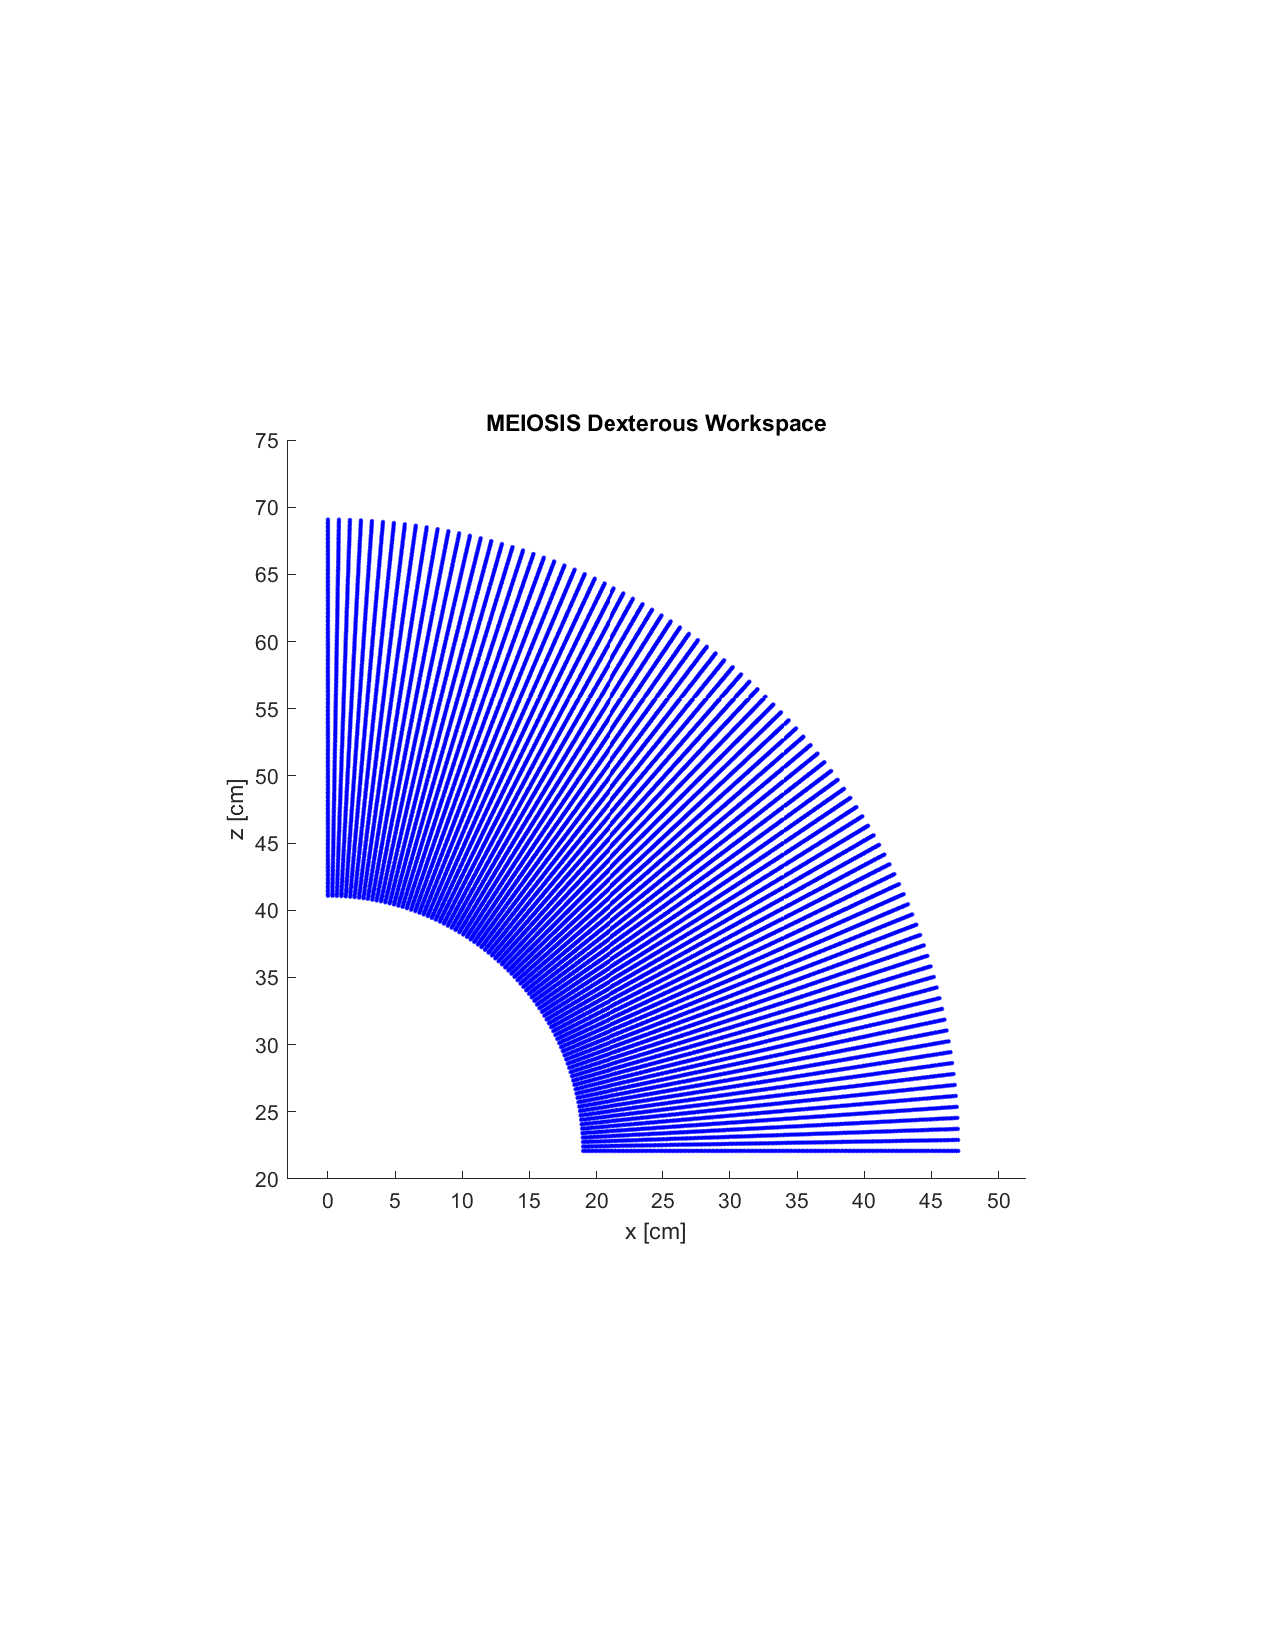
\includegraphics[frame,width=.75\textwidth]{dex}
%   \caption{Cross Section of Dexterous Workspace Quadrant}
%   \label{fig:dex}
% \end{figure}
% \hiddenappsub{CAD Drawings}
% % \subsection{CAD Drawings}
% The complete drawing package is attached.
% 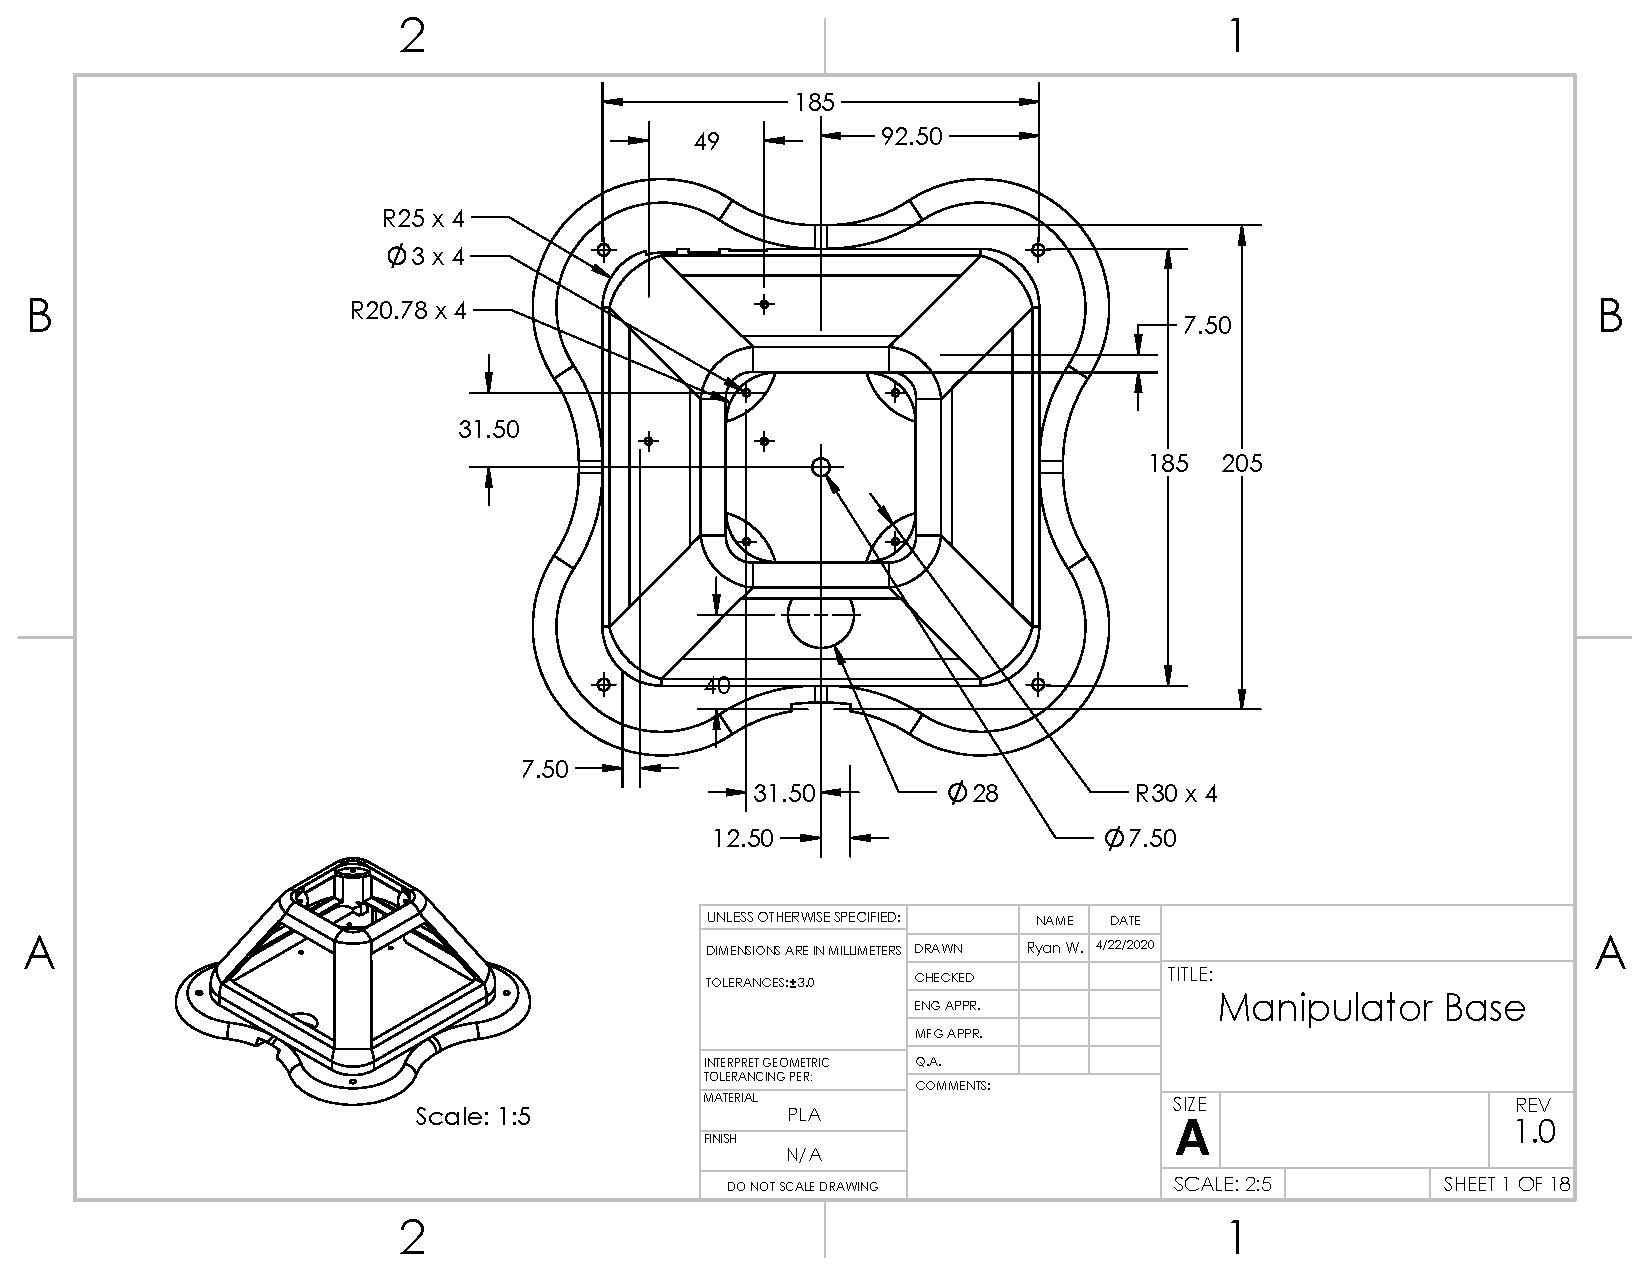
\includepdf[landscape,pages=-]{drawings}
% 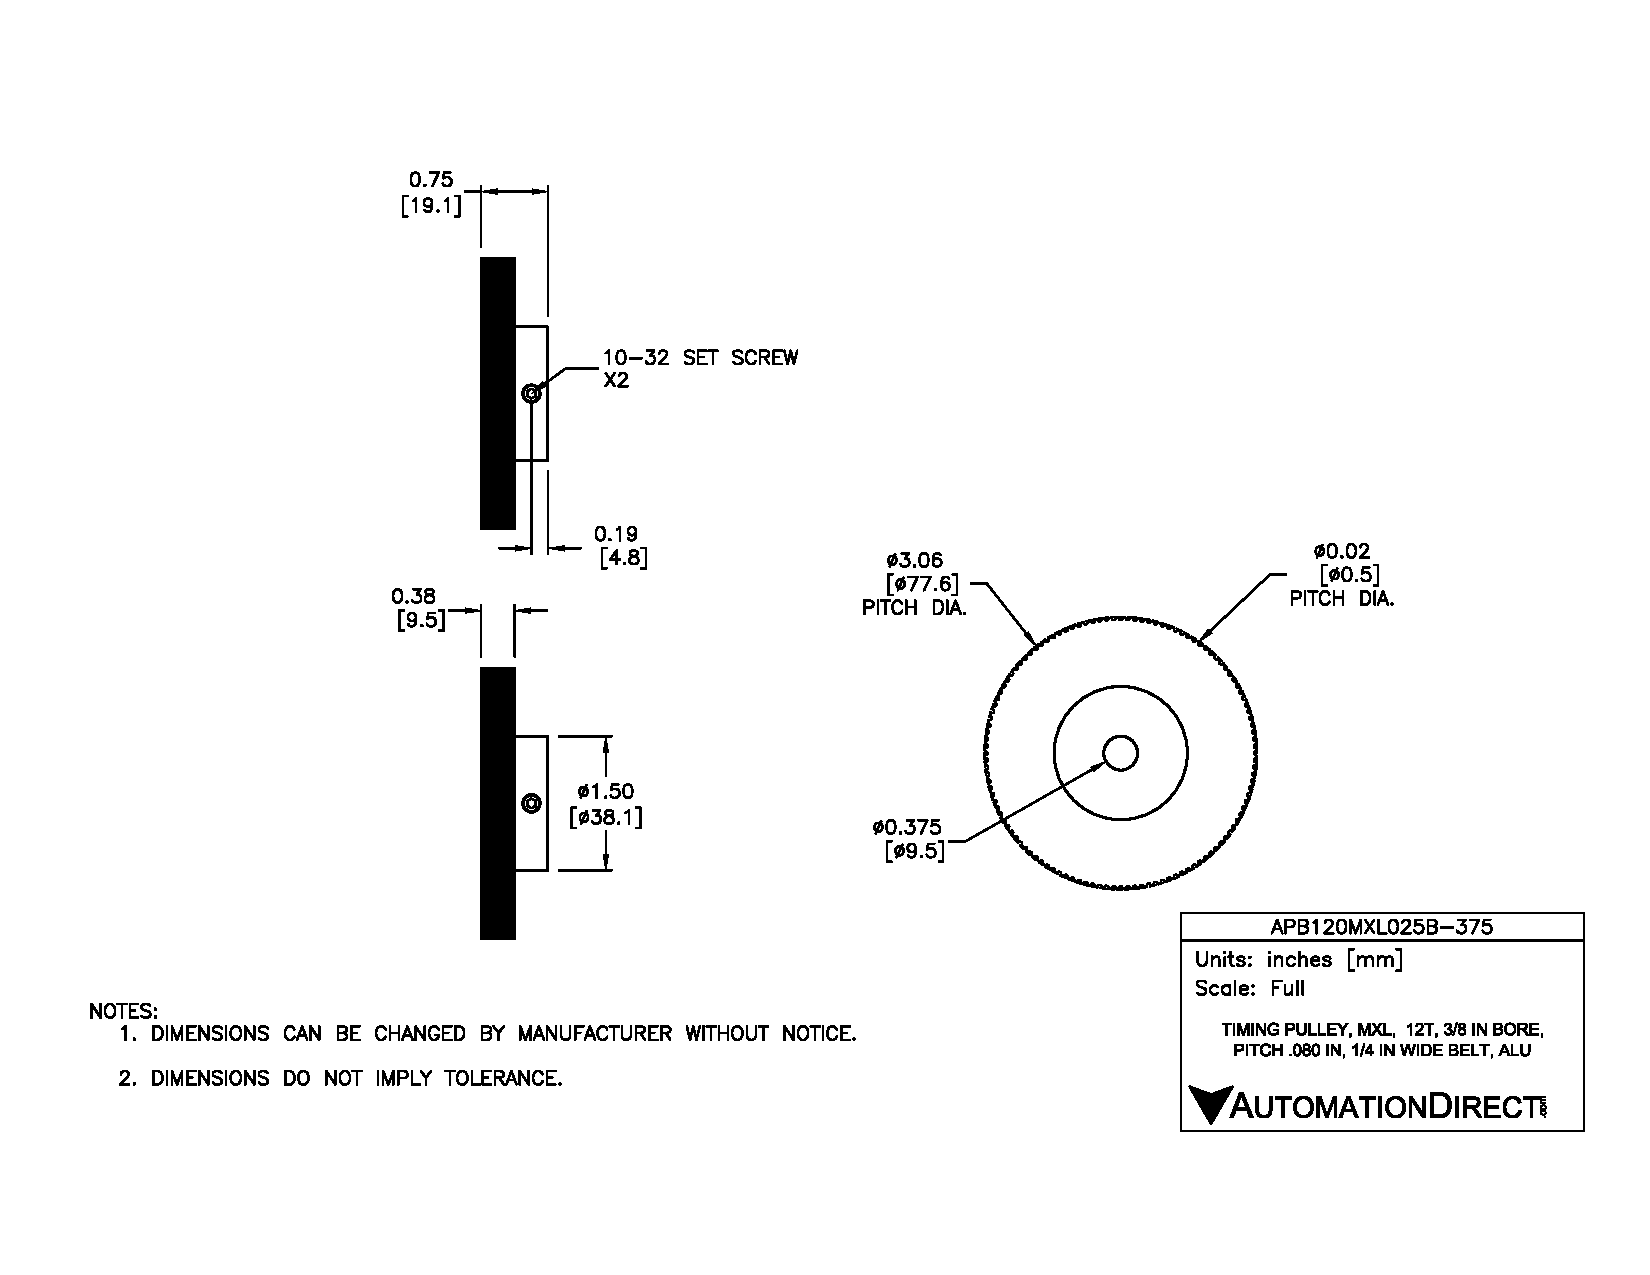
\includepdf[landscape,pages=-]{pulleys}
\hiddenappsub{Salient Code}
\begin{lstlisting}[frame=lines,style=Matlab-editor,basicstyle = \mlttfamily, label=code:mmodel, caption=Actuator Dynamics MATLAB Code]
% dynamixel motor model experiment
close all;clear;clc

% test loads mass moments of inertia
m = [.146 .088 0.108];          % mass (kg)
b = [.61277 .37227 0.28257];    % length (m)
h = [.01915 0.01915 0.0299];    % height (m)
J = (1/12)*m.*(h.^2 + b.^2);

% path to csv files relative to script
datapath = 'data/AX12A/';
files = dir(strcat(datapath,'*.csv'));
numFiles = length(files);
% initialize variables
[damp, wn, Tp] = deal(zeros(numFiles,1));

for ii = 1:numFiles
    % load experimental data, skip 5 header lines
        M = csvread(strcat(datapath, files(ii).name),5,0);
    % clean data by removing outliers
        nani = (find(diff(M(:,1)) > 100));
        M(nani,:) = [];
    % show response
         figure();
         plot(M(:,1),M(:,2))
         title('Experimental Data')
    % find % OS
        peak = max(M(:,2));                        % peak value
        peaki = find(M(:,2)==peak, 1, 'first');    % peak value index
        ss = M(end,2);                             % steady state
        os = ((peak - ss) / ss) * 100;             % % OS
    % damping ratio
        damp(ii) = -log(os/100) / sqrt(pi^2 + log(os/100)^2);
    % find where the motor begins responding
        start = M(find(diff(M(:,2)) > 1, 1, 'first'), 1);
    % time to peak
        Tp(ii) = (M(peaki,1) - start) / 1000;
    % natural frequency
        wn(ii) = pi / (sqrt(1 - damp(ii)^2)*Tp(ii));
end

sol = zeros(4,1);
% no load case, 2*zeta*omega_n
sol(1) = 2*mean(damp(end-2:end))*mean(wn(end-2:end));
% no load case, omega_n^2
sol(2) = mean(wn(end-2:end))^2;

% obtain average damping ratio and natural frequencies for load cases
zeta = [mean(damp(1:3));mean(damp(4:6));mean(damp(7:9))];
omegan = [mean(wn(1:3));mean(wn(4:6));mean(wn(7:9))];

alpha = 2.*zeta.*omegan;
beta = omegan.^2;
A = zeros(3,2);
b = zeros(3,1);

for jj = 1:3
    A(jj,:) = [1, -(alpha(jj)*J(jj) + beta(jj)*J(jj))];
    b(jj) = alpha(jj) + beta(jj);
end

sol(3:4) = A \ b;
\end{lstlisting}

\vspace{10ex}
%
% \begin{lstlisting}[frame=lines,style=Matlab-editor,basicstyle = \mlttfamily, caption=Forward Kinematics MATLAB Function]
function [r6,T6]= MeiosisFK(theta)

    %       Mapping between joint space and motor space
    N = 10;         %Gear Ratio
    A = [ 1/(2*N), 1/(2*N),   0, 0,   0,   0;
          1/(2*N),-1/(2*N),   0, 0,   0,   0;
                0,       0,-1/N, 0,   0,   0;
                0,       0,   0, 1,   0,   0;
                0,       0,   0, 0,-1/2, 1/2;
                0,       0,   0, 0, 1/2, 1/2];
    gamma = A*theta;

%     %Define Constants
%     LB = 12.275;
%     L1 = 0;
%     L2 = 25;
%     L3 = 20;
%     L4 = 7.2;
%     L5 = 0;
%     L6 = 5.3;

    %Relative Positions
    rBfromI = [ 0.00000000; 0.00000000; 0.00000000];
    r1fromB = [ 0.00000000; 0.00000000; 0.12275000];
    r2from1 = [ 0.00000000; 0.00000000; 0.00000000];
    r3from2 = [ 0.00000000; 0.25000000; 0.00000000];
    r4from3 = [ 0.00000000; 0.20000000; 0.00000000];
    r5from4 = [ 0.00000000; 0.07000000; 0.00000000];
    r6from5 = [ 0.00000000; 0.04750000; 0.00000000];
    %r7from6 = [0;       0;       0]; % dist. from 3rd wrist coor. frame to the end effector is 5.25 cm

    %Orientations wrt I:
    T1 = rotz(gamma(1));
    T2 = T1*rotx(gamma(2));
    T3 = T2*rotx(gamma(3));
    T4 = T3*roty(gamma(4));
    T5 = T4*rotx(gamma(5));
    T6 = T5*roty(gamma(6));

    %Positions wrt I:
    %rB = rBfromI;
    r1 = r1fromB;
    r2 = r1 + T1*r2from1;
    r3 = r2 + T2*r3from2;
    r4 = r3 + T3*r4from3;
    r5 = r4 + T4*r5from4;
    r6 = r5 + T5*r6from5;

end
\end{lstlisting}

% \vspace{10ex}
%
% \begin{lstlisting}[frame=lines,style=Matlab-editor,basicstyle = \mlttfamily, caption=Inverse Kinematics MATLAB Function]
function [theta, error] = MeiosisIK(pos,R)

    eOff = [0;47.5;0];
    npos = pos - R*eOff;
    xc = npos(1);
    yc = npos(2);
    zc = npos(3);
    L1 = 122.75;
    d = 0;
    L2 = 250;
    L3 = 270;

    % Inverse Position
    if (xc^2 + yc^2 -d^2) < 0
        theta = 1000*[1;1;1;1;1;1];
        error = 1;
    else
        t1 = atan2(yc,xc) - atan2(d,sqrt(xc^2 + yc^2 -d^2)) - pi/2;
        D = (xc^2 + yc^2 - d^2 + (zc - L1)^2 - L2^2 - L3^2)/(2*L2*L3);
        t3 = atan2(-sqrt(1-D^2),D);
        t2 = atan2(zc - L1,sqrt(xc^2 + yc^2 - d^2)) - atan2(L3*sin(t3),L2 + L3*cos(t3));

        % Inverse Orientation
        T3 = rotz(t1)*rotx(t2)*rotx(t3);
        T = T3.'*R;
        t6 = atan2(T(2,1),-T(2,3));
        t4 = atan2(T(1,2),T(3,2));
        %t4 = atan2(sin(t4),cos(t4));

        if sin(t4) > -10e-6 && sin(t4) < 10e-6
            t5 = atan2(T(3,2)/cos(t4),T(2,2));
        else
            t5 = atan2(T(1,2)/sin(t4),T(2,2));
        end

        gamma = [t1,t2,t3,t4,t5,t6].';

        %       Mapping between joint space and motor space
        N = 10;         %Gear Ratio
%         B = [ N, N, 0, 0, 0, 0;
%               N,-N, 0, 0, 0, 0;
%               0, 0,-N, 0, 0, 0;
%               0, 0, 0, 1, 0, 0;
%               0, 0, 0, 0,-1, 1;
%               0, 0, 0, 0, 1, 1];
        A = [ 1/(2*N), 1/(2*N),   0, 0,   0,   0;
          1/(2*N),-1/(2*N),   0, 0,   0,   0;
                0,       0,-1/N, 0,   0,   0;
                0,       0,   0, 1,   0,   0;
                0,       0,   0, 0,-1/2, 1/2;
                0,       0,   0, 0, 1/2, 1/2];

        theta = A\gamma;
        error = 0;
    end
end
\end{lstlisting}

% \vspace{10ex}
%
% \begin{lstlisting}[frame=lines,style=Matlab-editor,basicstyle = \mlttfamily, caption=Closed Loop Animation]
% Closed Loop Animation
% 11/11/2019
%   Adapted from code written by: Zack Johnson and Edward Pierce

clear all
close all
clc

dt = 0.01;                    %Integration timestep
delta_t = 4;                  %Animation timestep
t = 0:dt:40;                  %Simulation time array
b = zeros(12);                %Pre-allocate state variable for all time

%Define Desired Coordinates and Desired Joint angles
[xDes,yDes,zDes,gammad] = Meiosis_Name();
r6d = MeiosisFK(gammad(:,1));

%Define initial conditions
b(:,1) = [0;0;0;0;0;0;0;0;0;0;0;0];     %Initial position and velocity

%Define Control Parameters
tolerance = .001*ones(3,1);

jj = 1;

for ii = 1:(length(t)-1)

gamma = b(1:6,ii);
r6 = MeiosisFK(gamma);
if (abs(r6(3)) < .001)
    ink(:,ii) = r6;         %Keep track of where the marker writes
    draw(ii) = 1;           %Keep track of when the marker writes
else
    ink(:,ii) = [0;0;0];
    draw(ii) = 0;
end
Xe = r6 - r6d;

if (abs(Xe) <= tolerance)
    jj = jj + 1;
    if jj > length(gammad)
        break
    end
    r6d = MeiosisFK(gammad(:,jj));
end
gammadMat(:,ii) = gammad(:,jj);

k1 = Meiosis_robot1(b(:,ii),gammad(:,jj));
k2 = Meiosis_robot1(b(:,ii) + k1.*dt/2,gammad(:,jj));
k3 = Meiosis_robot1(b(:,ii) + k2.*dt/2,gammad(:,jj));
k4 = Meiosis_robot1(b(:,ii) + k3.*dt,gammad(:,jj));
b(:,ii+1) = b(:,ii) + dt*(k1./6 + k2./3 + k3./3 + k4./6);


end

% Animation
x = ink(1,:);
y = ink(2,:);
%z = r6Mat(3,:);
z = zeros(size(x));

figure('Name','Closed-Loop Animation','NumberTitle','off')
ii = 1;
for jj = 1:delta_t:29%(length(b))
%for jj = (length(b)-1):length(b)
clf(gcf)
plot3(x(1:jj),y(1:jj),z(1:jj),'r.')
hold on
Meiosis_draw2(b(1:6,jj))
F(ii) = getframe(gcf);
pause(0.001)
ii = ii + 1;
end

%      % Uncomment the following section to store the animation as a video
% writerObj = VideoWriter('DifferentialAnimation.avi');
% writerObj.FrameRate = 1/(dt*delta_t);
% open(writerObj);
%
% % write the frames to the video
% for i=1:length(F)
%     writeVideo(writerObj, F(i));
% end
%close(writerObj);

figure('Renderer', 'painters', 'Position', [10 100 700 700],'Name','Joint Angles vs. Time','NumberTitle','off')
Meiosis_Joint_Angle_plot(b(1:6,1:length(gammadMat)),gammadMat,t(1:length(gammadMat)),'Joint Angles vs. Time')
print('JointAnglePlot.pdf','-dpdf')
\end{lstlisting}

% \vspace{10ex}
%
% \begin{lstlisting}[frame=lines,style=Matlab-editor,basicstyle = \mlttfamily, caption=MEIOSIS Drawing Function]
function Meiosis_draw2(gamma,clr)

    if exist('clr','var')
        if (clr == 'clear') | (clr == 'Clear')
            clf(gcf);
        end
    end

    Floor_v = [-.3 .4 0;...
                .3 .4 0;...
               -.3 .2 0;...
                .3 .2 0];
    Floor_f = [1 2 4 3];

    set(gcf, 'Position', [50, 50, 950, 900])
    hold on
    patch('Faces',Floor_f,'Vertices',Floor_v,'EdgeColor','None','FaceColor','white');%,'FaceAlpha',.5);


    [Base,  Base_f]    = stlread('STL/Base.stl');
    [Link1, Link1_f]   = stlread('STL/Link1.stl');
    [Link2, Link2_f]   = stlread('STL/Link2new.stl');
    [Link3, Link3_f]   = stlread('STL/Link3.stl');
    [Link4, Link4_f]   = stlread('STL/Link4.stl');
    [Link5, Link5_f]   = stlread('STL/Link5.stl');
    [Link6, Link6_f]   = stlread('STL/Link6.stl');
    [Gear1, Gear1_f]   = stlread('STL/Gear1.stl');
    [Gear2, Gear2_f]   = stlread('STL/Gear2.stl');
    [Gear3, Gear3_f]   = stlread('STL/Gear3.stl');
    [Gear4, Gear4_f]   = stlread('STL/Gear4.stl');
    [Link2tube, Link2tube_f]   = stlread('STL/Link2tube.stl');
    [Link3tube, Link3tube_f]   = stlread('STL/Link3tube.stl');
    [Pulley1, Pulley1_f] = stlread('STL/Pulley1.stl');
    [Pulley2, Pulley2_f] = stlread('STL/Pulley2.stl');
    [Link4motors, Link4motors_f]   = stlread('STL/Link4motors.stl');
    [Link6motor, Link6motor_f]   = stlread('STL/Link6motor.stl');
    [Link2belt, Link2belt_f]   = stlread('STL/Link2belt.stl');
    [Link3belt, Link3belt_f]   = stlread('STL/Link3belt.stl');

    %          Forward kinematics
    %Relative Positions
    rBfromI =  [ 0.00000000; 0.00000000; 0.00000000];
    r1fromB =  [ 0.00000000; 0.00000000; 0.12275000];
    r2from1 =  [ 0.00000000; 0.00000000; 0.00000000];
    r3from2 =  [ 0.00000000; 0.26000000; 0.00000000];
    r4from3 =  [ 0.00000000; 0.20000000; 0.00000000];
    r5from4 =  [ 0.00000000; 0.07000000; 0.00000000];
    r6from5 =  [ 0.00000000; 0.09600000; 0.00000000];
    rG1from1 = [ 0.09055000; 0.00000000; 0.00000000];
    rG2from1 = [-0.09055000; 0.00000000; 0.00000000];
    rG3from5 = [ 0.04700000; 0.00000000; 0.00000000];
    rG4from5 = [-0.04700000; 0.00000000; 0.00000000];

    %Orientations wrt I
    TB = eye(3);
    T{1} = TB*rotz(gamma(1));
    T{2} = T{1}*rotx(gamma(2));
    T{3} = T{2}*rotx(gamma(3));
    T{4} = T{3}*roty(gamma(4));
    T{5} = T{4}*rotx(gamma(5));
    T{6} = T{5}*roty(gamma(6));
    T{7} = T{1}*rotx(-gamma(1));        %Gear 1
    T{8} = T{1}*rotx(gamma(1));         %Gear 2
    T{9} = T{5}*rotx(-gamma(6));        %Gear 3
    T{10} = T{5}*rotx(gamma(6));        %Gear 4

    %Positions wrt I
    rB = rBfromI;
    r{1} = rB + TB*r1fromB;
    r{2} = r{1} + T{1}*r2from1;
    r{3} = r{2} + T{2}*r3from2;
    r{4} = r{3} + T{3}*r4from3;
    r{5} = r{4} + T{4}*r5from4;
    r{6} = r{5} + T{5}*r6from5;
    r{7} = r{1} + T{1}*rG1from1;        %Gear 1
    r{8} = r{1} + T{1}*rG2from1;        %Gear 2
    r{9} = r{5} + T{5}*rG3from5;        %Gear 3
    r{10}= r{5} + T{5}*rG4from5;        %Gear 4

    %Transform the stl coordinates based upon FK
    Base_v   = repmat(rB,1,length(Base)) + Base';
    Link1_v  = repmat(r{1},1,length(Link1)) + T{1}*Link1';
    Link2_v  = repmat(r{2},1,length(Link2)) + T{2}*Link2';
    Link2tube_v  = repmat(r{2},1,length(Link2tube)) + T{2}*Link2tube';
    Link3_v  = repmat(r{3},1,length(Link3)) + T{3}*Link3';
    Link3tube_v  = repmat(r{3},1,length(Link3tube)) + T{3}*Link3tube';
    Link4_v  = repmat(r{4},1,length(Link4)) + T{4}*Link4';
    Link5_v  = repmat(r{5},1,length(Link5)) + T{5}*Link5';
    Link6_v  = repmat(r{6},1,length(Link6)) + T{6}*Link6';
    Gear1_v  = repmat(r{7},1,length(Gear1)) + T{7}*Gear1';
    Gear2_v  = repmat(r{8},1,length(Gear2)) + T{8}*Gear2';
    Gear3_v  = repmat(r{9},1,length(Gear3)) + T{9}*Gear3';
    Gear4_v  = repmat(r{10},1,length(Gear4)) + T{10}*Gear4';
    Pulley1_v  = repmat(r{7},1,length(Pulley1)) + T{7}*Pulley1';
    Pulley2_v  = repmat(r{8},1,length(Pulley2)) + T{8}*Pulley2';
    Link4motors_v  = repmat(r{4},1,length(Link4motors)) + T{4}*Link4motors';
    Link6motor_v  = repmat(r{6},1,length(Link6motor)) + T{6}*Link6motor';
    Link2belt_v  = repmat(r{2},1,length(Link2belt)) + T{2}*Link2belt';
    Link3belt_v  = repmat(r{3},1,length(Link3belt)) + T{3}*Link3belt';

    patch('Faces',Base_f, 'Vertices',Base_v', 'EdgeColor','None','FaceColor',[0 0.082353 1]);
    patch('Faces',Link1_f,'Vertices',Link1_v','EdgeColor','None','FaceColor',[0.901961 0.756863 0.035294]);
    patch('Faces',Link2_f,'Vertices',Link2_v','EdgeColor','None','FaceColor',[0 0.082353 1]);
    patch('Faces',Link2tube_f,'Vertices',Link2tube_v','EdgeColor','None','FaceColor',[0.5774    0.5774    0.5774]);
    patch('Faces',Link3_f,'Vertices',Link3_v','EdgeColor','None','FaceColor',[0.901961 0.756863 0.035294]);
    patch('Faces',Link3tube_f,'Vertices',Link3tube_v','EdgeColor','None','FaceColor',[0.5774    0.5774    0.5774]);
    patch('Faces',Link4_f,'Vertices',Link4_v','EdgeColor','None','FaceColor',[0 0.082353 1]);
    patch('Faces',Link5_f,'Vertices',Link5_v','EdgeColor','None','FaceColor',[0.901961 0.756863 0.035294]);
    patch('Faces',Link6_f,'Vertices',Link6_v','EdgeColor','None','FaceColor',[1 0.082353 0.082353]);
    patch('Faces',Gear1_f,'Vertices',Gear1_v','EdgeColor','None','FaceColor',[1 0.082353 0.082353]);
    patch('Faces',Gear2_f,'Vertices',Gear2_v','EdgeColor','None','FaceColor',[1 0.082353 0.082353]);
    patch('Faces',Gear3_f,'Vertices',Gear3_v','EdgeColor','None','FaceColor',[1 0.082353 0.082353]);
    patch('Faces',Gear4_f,'Vertices',Gear4_v','EdgeColor','None','FaceColor',[1 0.082353 0.082353]);
    patch('Faces',Pulley1_f,'Vertices',Pulley1_v','EdgeColor','None','FaceColor',[0.5774    0.5774    0.5774]);
    patch('Faces',Pulley2_f,'Vertices',Pulley2_v','EdgeColor','None','FaceColor',[0.5774    0.5774    0.5774]);
    patch('Faces',Link4motors_f,'Vertices',Link4motors_v','EdgeColor','None','FaceColor',[0.5774    0.5774    0.5774]);
    patch('Faces',Link6motor_f,'Vertices',Link6motor_v','EdgeColor','None','FaceColor',[0.5774    0.5774    0.5774]);
    patch('Faces',Link2belt_f,'Vertices',Link2belt_v','EdgeColor','None','FaceColor',[0 0 0]);
    patch('Faces',Link3belt_f,'Vertices',Link3belt_v','EdgeColor','None','FaceColor',[0 0 0]);

    axis equal
    camlight(180,90)
    set(gca,'xtick',[])
    set(gca,'xticklabel',[])
    set(gca,'XColor','none')
    set(gca,'ytick',[])
    set(gca,'yticklabel',[])
    set(gca,'YColor','none')
    set(gca,'ztick',[])
    set(gca,'zticklabel',[])
    set(gca,'ZColor','none')
    set(gca,'Color','none')

    set(gca,'projection','perspective')
    view(140,45)
    axis([-0.4 0.4 -0.2 0.7 0 0.4])
    %axis([-.1 .1 -.1 .1 0 .2])

    hold off
end
\end{lstlisting}

% \vspace{10ex}
%
% \begin{lstlisting}[frame=lines,style=Matlab-editor,basicstyle = \mlttfamily, caption={H, D, and G Calculations}]
function [H, d, G] = Meiosis_HdG(gamma,gammadot)

    %       Mass Parameters
    %Mass(kg)
    m{1} = 0.13954848;      %Link 1
    m{2} = 1.14358921;      %Link 2
    m{3} = 1.00606970;      %Link 3
    m{4} = 0.26834265;      %Link 4
    m{5} = 0.03933179;      %Link 5
    m{6} = 0.19893937;
    m{7} = 0.24224704;      %Gear 1
    m{8} = 0.24224704;      %Gear 2
    m{9} = 0.05035795;      %Gear 3
    m{10} = 0.05035795;

    %Center of mass for each link (m)
    rcm{1} = [ 0.00000000; 0.00000000;-0.02792483];     %Link 1
    rcm{2} = [ 0.00007758; 0.15623908;-0.00011610];     %Link 2
    rcm{3} = [-0.01528806; 0.07006082; 0.00110335];     %Link 3
    rcm{4} = [ 0.00000000; 0.03163485; 0.00000000];     %Link 4
    rcm{5} = [ 0.00000000; 0.00630115; 0.00000000];     %Link 5
    rcm{6} = [ 0.00000000;-0.03626349;-0.00034373];     %Link 6
    rcm{7} = [-0.02271539;-0.00001560; 0.00001565];     %Gear 1
    rcm{8} = [ 0.02271539;-0.00001560;-0.00001565];     %Gear 2
    rcm{9} = [-0.00678010; 0.00000000; 0.00000000];     %Gear 3
    rcm{10}= [ 0.00678010; 0.00000000; 0.00000000];     %Gear 4

    Gam{1} = rcm{1}*m{1};
    Gam{2} = rcm{2}*m{2};
    Gam{3} = rcm{3}*m{3};
    Gam{4} = rcm{4}*m{4};
    Gam{5} = rcm{5}*m{5};
    Gam{6} = rcm{6}*m{6};
    Gam{7} = rcm{7}*m{7};
    Gam{8} = rcm{8}*m{8};
    Gam{9} = rcm{9}*m{9};
    Gam{10} = rcm{10}*m{10};

    %Inertia Matrices
	J{1} = [ 0.00015462  0.00000000  0.00000000;        %Link 1
	         0.00000000	 0.00016692  0.00000000;
	         0.00000000	 0.00000000  0.00003819];
    J{2} = [ 0.03894999 -0.00002305  0.00000000;        %Link 2
            -0.00002305  0.00589287  0.00001585;
             0.00000000  0.00001585  0.04414151];
    J{3} = [ 0.01143098  0.00169728  0.00000008;        %Link 3
	         0.00169728	 0.00185484 -0.00021794;
	         0.00000008	-0.00021794  0.01259229];
    J{4} = [ 0.00063966  0.00000000  0.00000000;        %Link 4
	         0.00000000	 0.00069715  0.00000000;
	         0.00000000	 0.00000000  0.00108401];
    J{5} = [ 0.00000851  0.00000000  0.00000000;        %Link 5
	         0.00000000	 0.00001467  0.00000000;
	         0.00000000	 0.00000000  0.00002081];
    J{6} = [ 0.00036378  0.00000000  0.00000000;        %Link 6
	         0.00000000	 0.00007212 -0.00000173;
	         0.00000000	-0.00000173  0.00034916];
    J{7} = [ 0.00014269 -0.00000005  0.00000005;        %Gear 1
	        -0.00000005	 0.00029726  0.00000000;
	         0.00000005	 0.00000000  0.00029726];
    J{8} = [ 0.00014269  0.00000005  0.00000005;        %Gear 2
	         0.00000005	 0.00029726  0.00000000;
	         0.00000005	 0.00000000  0.00029726];
    J{9} = [ 0.00003333  0.00000000  0.00000000;        %Gear 3
	         0.00000000	 0.00001986  0.00000000;
	         0.00000000	 0.00000000  0.00001986];
    J{10}= [ 0.00003333  0.00000000  0.00000000;        %Gear 4
	         0.00000000	 0.00001986  0.00000000;
	         0.00000000	 0.00000000  0.00001986];


    %          Forward kinematics
    %Relative Positions
    rBfromI =  [ 0.00000000; 0.00000000; 0.00000000];
    r1fromB =  [ 0.00000000; 0.00000000; 0.12275000];
    r2from1 =  [ 0.00000000; 0.00000000; 0.00000000];
    r3from2 =  [ 0.00000000; 0.26000000; 0.00000000];
    r4from3 =  [ 0.00000000; 0.20000000; 0.00000000];
    r5from4 =  [ 0.00000000; 0.07000000; 0.00000000];
    r6from5 =  [ 0.00000000; 0.09600000; 0.00000000];
    rG1from1 = [ 0.09055000; 0.00000000; 0.00000000];
    rG2from1 = [-0.09055000; 0.00000000; 0.00000000];
    rG3from5 = [ 0.04700000; 0.00000000; 0.00000000];
    rG4from5 = [-0.04700000; 0.00000000; 0.00000000];

    %Store orientations in cell array
    rn{1} = r1fromB;
    rn{2} = r2from1;
    rn{3} = r3from2;
    rn{4} = r4from3;
    rn{5} = r5from4;
    rn{6} = r6from5;
    rn{7} = rG1from1;
    rn{8} = rG2from1;
    rn{9} = rG3from5;
    rn{10} = rG4from5;

    %Orientations wrt I
    TB = eye(3);
    T{1} = TB*rotz(gamma(1));
    T{2} = T{1}*rotx(gamma(2));
    T{3} = T{2}*rotx(gamma(3));
    T{4} = T{3}*roty(gamma(4));
    T{5} = T{4}*rotx(gamma(5));
    T{6} = T{5}*roty(gamma(6));
    T{7} = T{1}*rotx(gamma(1));           %Gear 1
    T{8} = T{1}*rotx(-gamma(1));          %Gear 2
    T{9} = T{5}*rotx(-gamma(6));          %Gear 3
    T{10} = T{5}*rotx(gamma(6));          %Gear 4

    %Positions wrt I
    rB = rBfromI;
    r{1} = rB + TB*r1fromB;
    r{2} = r{1} + T{1}*r2from1;
    r{3} = r{2} + T{2}*r3from2;
    r{4} = r{3} + T{3}*r4from3;
    r{5} = r{4} + T{4}*r5from4;
    r{6} = r{5} + T{5}*r6from5;
    r{7} = r{1} + T{1}*rG1from1;        %Gear 1
    r{8} = r{1} + T{1}*rG2from1;        %Gear 2
    r{9} = r{5} + T{5}*rG3from5;        %Gear 3
    r{10}= r{5} + T{5}*rG4from5;        %Gear 4


    %              Recursive Kinematics
    Jb0 = zeros(6);
    Jbdot0 = zeros(6);

    for ii = 1:10
        if ii == 1
            Jmat = Jb0;
            wI = Jmat(1:3,:)*gammadot;
            [Jb{ii},Jbdot{ii}] = Next_GeoJac_Meiosis(Jb0,Jbdot0,gamma,gammadot,TB,rn{ii},zeros(3,1),wI,ii);
        elseif ii == 7
            Jmat = Jb{1};
            wI = Jmat(1:3,:)*gammadot;
            [Jb{ii},Jbdot{ii}] = Next_GeoJac_Meiosis(Jb{1},Jbdot{1},gamma,gammadot,T{1},rn{ii},zeros(3,1),wI,ii);
        elseif ii == 8
            Jmat = Jb{1};
            wI = Jmat(1:3,:)*gammadot;
            [Jb{ii},Jbdot{ii}] = Next_GeoJac_Meiosis(Jb{1},Jbdot{1},gamma,gammadot,T{1},rn{ii},zeros(3,1),wI,ii);
        elseif ii == 9
            Jmat = Jb{5};
            wI = Jmat(1:3,:)*gammadot;
            [Jb{ii},Jbdot{ii}] = Next_GeoJac_Meiosis(Jb{1},Jbdot{5},gamma,gammadot,T{5},rn{ii},zeros(3,1),wI,ii);
        elseif ii == 10
            Jmat = Jb{5};
            wI = Jmat(1:3,:)*gammadot;
            [Jb{ii},Jbdot{ii}] = Next_GeoJac_Meiosis(Jb{1},Jbdot{5},gamma,gammadot,T{5},rn{ii},zeros(3,1),wI,ii);
        else
            Jmat = Jb{ii-1};
            wI = Jmat(1:3,:)*gammadot;
            [Jb{ii},Jbdot{ii}] = Next_GeoJac_Meiosis(Jb{ii-1},Jbdot{ii-1},gamma,gammadot,T{ii-1},rn{ii},zeros(3,1),wI,ii);
        end

        Jmat = Jb{ii};
        wI = Jmat(1:3,:)*gammadot;

        Hmat = Jb{ii}.'*[J{ii},skew(Gam{ii})*T{ii}.';T{ii}*skew(Gam{ii}).',m{ii}*eye(3)]*Jb{ii};
        dvec = Jb{ii}.'*[J{ii},skew(Gam{ii})*T{ii}.';T{ii}*skew(Gam{ii}).',m{ii}*eye(3)]*Jbdot{ii}*gammadot + Jb{ii}.'*[cross(wI,J{ii}*wI);T{ii}*cross(wI,cross(wI,Gam{ii}))];
        g = Jb{ii}.'*[cross(rcm{ii},T{ii}.'*[0;0;-m{ii}*9.81]);[0;0;-m{ii}*9.81]];

        if ii == 1
            H = Hmat;
            d = dvec;
            G = g;
        else
            H = H + Hmat;
            d = d + dvec;
            G = G + g;
        end
    end

end
\end{lstlisting}

% \vspace{10ex}
%
% \begin{lstlisting}[frame=lines,style=Matlab-editor,basicstyle = \mlttfamily, caption=Joint Angle Plotting Code]
function Meiosis_Joint_Angle_plot(b,gammad,t,Title)

    % Plot joint angle 1
    subplot(4,2,1)
    hold on
    plot(t, b(1,:),'b');
    plot(t, gammad(1,:),'r--')
    title('First Joint Angle vs. Time');
    xlabel('Time (s)');
    ylabel('\theta_1 (rad)');
    legend('\theta','\theta_d')

    % Plot joint angle 2
    subplot(4,2,2)
    hold on
    plot(t, b(2,:),'b')
    plot(t, gammad(2,:),'r--')
    title('Second Joint Angle vs. Time');
    xlabel('Time (s)');
    ylabel('\theta_2 (rad)');
    legend('\theta','\theta_d','Location','Southeast')

    % Plot joint 3 movment
    subplot(4,2,3)
    hold on
    plot(t, b(3,:),'b')
    plot(t, gammad(3,:),'r--')
    title('Third Joint Angle vs. Time');
    xlabel('Time (s)');
    ylabel('\theta_3 (rad)');
    legend('\theta','\theta_d')

    % Plot joint 4 movment
    subplot(4,2,4)
    hold on
    plot(t, b(4,:),'b')
    plot(t, gammad(4,:),'r--')
    title('Fourth Joint Angle vs. Time');
    xlabel('Time (s)');
    ylabel('\theta_4 (rad)');
    legend('\theta','\theta_d','Location','Southeast')

    % Plot joint 5 movment
    subplot(4,2,5)
    hold on
    plot(t, b(5,:),'b')
    plot(t, gammad(5,:),'r--')
    title('Fifth Joint Angle vs. Time');
    xlabel('Time (s)');
    ylabel('\theta_5 (rad)');
    legend('\theta','\theta_d','Location','Southeast')

    % Plot joint 6 movment
    subplot(4,2,6)
    hold on
    plot(t, b(6,:),'b')
    plot(t, gammad(6,:),'r--')
    title('Sixth Joint Angle vs. Time');
    xlabel('Time (s)');
    ylabel('\theta_6 (rad)');
    legend('\theta','\theta_d','Location','Southeast')


%     annotation('textbox', [0 0.9 1 0.1], ...
%     'String', Title, ...
%     'EdgeColor', 'none', ...
%     'HorizontalAlignment', 'center')

end
\end{lstlisting}

% \vspace{10ex}
%
% \begin{lstlisting}[frame=lines,style=Matlab-editor,basicstyle = \mlttfamily, caption=MEIOSIS Name Plotting]
function [xDes,yDes,zDes,thetad] = Meiosis_Name2()

    %Define Desired Workspace Coordinates
    [xM,yM,zM] = LetterM();
    [xE,yE,zE] = LetterE();
    [xI1,yI1,zI1] = LetterI1();
    [xO,yO,zO] = LetterO();
    [xS1,yS1,zS1] = LetterS1();
    [xI2,yI2,zI2] = LetterI2();
    [xS2,yS2,zS2] = LetterS2();

    xDes = [xM,xE,xI1,xO,xS1,xI2,xS2];
    yDes = [yM,yE,yI1,yO,yS1,yI2,yS2];
    zDes = [zM,zE,zI1,zO,zS1,zI2,zS2];

    R = rotx(-pi/2);


    %Calculate Joint Angles
    for ii = 1:length(xDes)
        [thetad(:,ii),errorCheck] = MeiosisIK([xDes(ii);yDes(ii);zDes(ii)],R);
        if errorCheck == 1
            break
        end
    end
end

function [x,y,z] = LetterM()

    %Define Desired Workspace Coordinates
    x = [ 270, 270, 240, ];
    y = [ 290, 290, 250, ];
    z = [  10,   0, ];

end

function [x,y,z] = LetterE()

    %Define Desired Workspace Coordinates
    x = [210, 210, 210, 150, 150, 200, 200, 170, 170, 200, 200, 150, 150, 210, 210];
    y = [260, 260, 340, 340, 330, 330, 300, 300, 290, 290, 270, 270, 260, 260, 260];
    z = [ 10,   0,   0,   0,   0,   0,   0,   0,   0,   0,   0,   0,   0,   0,  10];

end

function [x,y,z] = LetterI1()

    %Define Desired Workspace Coordinates
    x = [130, 130, 130, 110, 110, 130, 130,  80,  80, 100, 100,  80,  80, 130, 130];
    y = [260, 260, 270, 270, 330, 330, 340, 340, 330, 330, 270, 270, 260, 260, 260];
    z = [ 10,   0,   0,   0,   0,   0,   0,   0,   0,   0,   0,   0,   0,   0,  10];

end

function [x,y,z] = LetterO()

    %Define Desired Workspace Coordinates
    x = [ 60,  60,  60,   0,   0,  60,  60,  50,  50,  50,  10,  10,  50,  50];
    y = [260, 260, 340, 340, 260, 260, 260, 270, 270, 330, 330, 270, 270, 270];
    z = [ 10,   0,   0,   0,   0,   0,  10,  10,   0,   0,   0,   0,   0,  10];

end

function [x,y,z] = LetterS1()

    %Define Desired Workspace Coordinates
    x = [-20, -20, -20, -50, -50, -20, -20, -60, -60, -30, -30, -60, -60, -20, -20];
    y = [260, 260, 300, 300, 330, 330, 340, 340, 290, 290, 270, 270, 260, 260, 260];
    z = [ 10,   0,   0,   0,   0,   0,   0,   0,   0,   0,   0,   0,   0,   0,  10];

end

function [x,y,z] = LetterI2()

    %Define Desired Workspace Coordinates
    [x,y,z] = LetterI1();
    x = x - 210;

end

function [x,y,z] = LetterS2()

    %Define Desired Workspace Coordinates
    [x,y,z] = LetterS1();
    x = x - 130;

end


\end{lstlisting}

% \vspace{10ex}
%
% \begin{lstlisting}[frame=lines,style=Matlab-editor,basicstyle = \mlttfamily, caption=MEIOSIS Robot State Calculator]
function bdot = Meiosis_robot1(b,gammad)

    %Preallocate variables
    bdot = zeros(12,1);

    %Variable reassignments
    gamma = b(1:6);
    gammadot = b(7:12);

    [H,d,G] = Meiosis_HdG(gamma,gammadot);
    C1 = diag((1 / 82.5459264810444)*[1 1 1 1 1 1]);
    C2 = diag((13.4787019763844 / 82.5459264810444)*[1 1 1 1 1 1]);
    C3 = diag((88.3252169803572 / 82.5459264810444)*[1 1 1 1 1 1]);

    N = 10;  %Gear Ratio
    A = [ 1/(2*N), 1/(2*N),   0, 0,   0,   0;
          1/(2*N),-1/(2*N),   0, 0,   0,   0;
                0,       0,-1/N, 0,   0,   0;
                0,       0,   0, 1,   0,   0;
                0,       0,   0, 0,-1/2, 1/2;
                0,       0,   0, 0, 1/2, 1/2];

    bdot(1:6) = b(7:12);
    u = (A.'\C3)\(G + d) + A\gammad;
    bdot(7:12) = (H + A.'\C1/A)\(-d - G - A\C2/A*gammadot - A.'\C3/A*gamma + A.'\C3*u);

end
\end{lstlisting}

% \vspace{10ex}
%
% \begin{lstlisting}[frame=lines,style=Matlab-editor,basicstyle = \mlttfamily, caption=MEIOSIS Velocity Calculator]
function [dotr,w] = MeiosisVelocity(T,r,gamma,dotgamma)

    dotr = simplify(jacobian(r,gamma)*dotgamma);

    Jw = [T(:,3).'*jacobian(T(:,2),gamma);...
          T(:,1).'*jacobian(T(:,3),gamma);...
          T(:,2).'*jacobian(T(:,1),gamma)];

    M = simplify(Jw,'steps',200,'criterion','preferReal');

    w = simplify(M*dotgamma);

end
\end{lstlisting}

% \vspace{10ex}
%
% \begin{lstlisting}[frame=lines,style=Matlab-editor,basicstyle = \mlttfamily, caption=Geometric Jacobian Calculator]
function [JbN,JbNdot] = Next_GeoJac_Meiosis(Jb,Jbdot,gamma,gammadot,TI,rn,rndot,wI,link)

    Ihat = zeros(3,length(gamma));
    Itilda = zeros(3,length(gamma));

    %link = 8 corresponds to the screen
    %
    switch link
        case 1
            Ihat(3,1) = 1;
            Tn = rotz(gamma(1));
        case 2
            Ihat(1,2) = 1;
            Tn = rotx(gamma(2));
        case 3
            Ihat(1,3) = 1;
            Tn = rotx(gamma(3));
        case 4
            Ihat(2,4) = 1;
            Tn = roty(gamma(4));
        case 5
            Ihat(1,5) = 1;
            Tn = rotx(gamma(5));
        case 6
            Ihat(2,6) = 1;
            Tn = roty(gamma(6));
        case 7                      %Gear 1
            Ihat(1,1) = 1;
            Tn = rotx(gamma(1));
        case 8                      %Gear 2
            Ihat(1,1) = 1;
            Tn = rotx(-gamma(1));
        case 9                      %Gear 3
            Ihat(1,1) = 1;
            Tn = rotx(-gamma(6));
        case 10                     %Gear 4
            Ihat(1,1) = 1;
            Tn = rotx(gamma(6));

    end

    %GeoJac Matrices
    mat1 = [Tn.',zeros(3);-TI*skew(rn),eye(3)];
    mat2 = [Ihat;TI*Itilda];

    JbN = mat1*Jb + mat2;

    %GeoJacdot matrices
    mat1 = [           -skew(Ihat*gammadot)*(Tn.'), zeros(3);
            -TI*skew(wI)*skew(rn) - TI*skew(rndot), zeros(3)];
    mat2 = [        Tn.', zeros(3);
            -TI*skew(rn), eye(3)];
    mat3 = [           zeros(3,6);
            TI*skew(wI)*Itilda];

    JbNdot = mat1*Jb + mat2*Jbdot + mat3;

end
\end{lstlisting}

% \vspace{10ex}
%
% \begin{lstlisting}[frame=lines,style=Matlab-editor,basicstyle = \mlttfamily, caption=Open-Loop Animation Code]
% Open Loop Animation
% 11/11/2019
%   Adapted from code written by: Zack Johnson and Edward Pierce

clear all
close all
clc

dt = 0.001;                     %Integration timestep
fr = 24;                        %Animation Framerate
delta_t = round(1/(dt*fr));     %Animation timestep
t = 0:dt:30;                    %simulation time array
b = zeros(12,length(t));        %pre-allocate motor angles for all time
Va = zeros(6,length(t));        %pre-allocate input torque for all time

%Define initial conditions
b(:,1) = [0;0;0;0;0;0;0;0;0;0;0;0];     %Initial position and velocity

for ii = 1:(length(t)-1)
k1 = Meiosis_robot1(b(:,ii),Va(:,ii));
k2 = Meiosis_robot1(b(:,ii) + k1.*dt/2,Va(:,ii));
k3 = Meiosis_robot1(b(:,ii) + k2.*dt/2,Va(:,ii));
k4 = Meiosis_robot1(b(:,ii) + k3.*dt,Va(:,ii));
b(:,ii+1) = b(:,ii) + dt*(k1./6 + k2./3 + k3./3 + k4./6);
ii/length(t)
end

% for ii = delta_t:delta_t:(length(b))
jj = 1;
for ii = 1:delta_t:length(b)
Meiosis_draw2(b(1:7,ii),'clear',t(ii))
F(jj) = getframe(gcf);
jj = jj + 1;
end

 % Uncomment the following section to store the animation as a video
writerObj = VideoWriter('OpenLoopAnimation.avi');
writerObj.FrameRate = fr;
open(writerObj);

% write the frames to the video
for i=1:length(F)
writeVideo(writerObj, F(i));
end
close(writerObj);

figure('Renderer', 'painters', 'Position', [10 100 700 700],'Name','Joint Angles vs. Time','NumberTitle','off')
Meiosis_Joint_Angle_plot(b(1:6,:),t(1:length(b)),'Joint Angles vs. Time')
print('JointAnglePlot.pdf','-dpdf')
\end{lstlisting}

% \vspace{10ex}
%
% \begin{lstlisting}[frame=lines,style=Matlab-editor,basicstyle = \mlttfamily, caption=Velocity Kinematics Code]
clear all
close all
clc

%Define Symbolic Variables
syms t1 t2 t3 t4 t5 t6 dt1 dt2 dt3 dt4 dt5 dt6 L1 L2 L3 L4 L5 L6
q = [t1 t2 t3 t4 t5 t6].';
dotq = [dt1 dt2 dt3 dt4 dt5 dt6].';

%Relative Positions
rBfromI = [  0;  0;  0];
r1fromB = [  0;  0; L1];    % Frame 1 is 122.75mm away from the Base frame in the Z direction
r2from1 = [  0;  0;  0];    % Frame 2 is centered on Frame 1
r3from2 = [  0; L2;  0];    % Frame 3 is 250mm away from Frame 2 in the Y direction
r4from3 = [  0; L3;  0];    % Frame 4 is 200mm away from Frame 3 in the Y direction
r5from4 = [  0; L4;  0];    % Frame 5 is 70mm away from Frame 4 in the Y direction
r6from5 = [  0; L6;  0];    % Frame 6 is 47.5mm away from Frame 5 in the Y direction

%Orientations wrt I:
T(:,:,1) = rotz(t1);
T(:,:,2) = T(:,:,1)*rotx(t2);
T(:,:,3) = T(:,:,2)*rotx(t3);
T(:,:,4) = T(:,:,3)*roty(t4);
T(:,:,5) = T(:,:,4)*rotx(t5);
T(:,:,6) = T(:,:,5)*roty(t6);

%Positions wrt I:
rB = rBfromI;
r(:,1) = rB + r1fromB;
r(:,2) = r(:,1) + T(:,:,1)*r2from1;
r(:,3) = r(:,2) + T(:,:,2)*r3from2;
r(:,4) = r(:,3) + T(:,:,3)*r4from3;
r(:,5) = r(:,4) + T(:,:,4)*r5from4;
r(:,6) = r(:,5) + T(:,:,5)*r6from5;


for ii = 1:6
    [dotr(:,ii),w(:,ii)] = MeiosisVelocity(T(:,:,ii),r(:,ii),q,dotq);
    disp(ii)
    disp(dotr(:,ii))
    disp(w(:,ii))

end

\end{lstlisting}

% \vspace{10ex}

% Code listing
%\begin{lstlisting}[frame=lines,style=Matlab-editor,basicstyle = \mlttfamily, caption=Example Code]
% Code Here
%\end{lstlisting}
% \includepdf[landscape,pages=-]{pdfname}

\end{document}
